% BROOMSHARING | DO AN MOBILE | BAN HIEU CHINH THEO 2 MAU
% AI_PROJECT: bia, cach trinh bay phu luc, lien ket va danh muc cuoi.
% FINAL_ANDROID: le trang, font, gian dong, thut dau dong, section va tham khao.
% Build: pdflatex main; biber main; pdflatex main; pdflatex main.
\documentclass[12pt,a4paper]{article}
\ifdefined\pdfminorversion\pdfminorversion=7\fi
\usepackage[utf8]{inputenc}
\usepackage[T1,T5]{fontenc}
\usepackage{mathptmx}
\usepackage{amsmath,amssymb}
\numberwithin{figure}{subsection}
\numberwithin{table}{subsection}
% FINAL_ANDROID: lề trang va line spacing giu nguyen.
\usepackage[top=2cm,bottom=2cm,left=3cm,right=2cm]{geometry}
\usepackage{setspace}
\setstretch{1.4}
\setlength{\parindent}{1.27cm}
\setlength{\parskip}{0pt}
\setcounter{tocdepth}{2} % Noi dung chinh gom section va subsection, khong nhieu tang TOC
% Khong dung indentfirst: doan dau ngay sau section / subsection sat le.
% Chi cac doan tiep theo thut 1.27cm theo LaTeX.
\usepackage{microtype}
\usepackage{enumitem}
\setlist[itemize,1]{label=\textbullet,leftmargin=*,itemsep=2pt,topsep=4pt}
\setlist[itemize,2]{label=$\circ$,leftmargin=*,itemsep=1pt}
\setlist[itemize,3]{label=--}
\usepackage[table]{xcolor}
\usepackage{booktabs,longtable,tabularx,array,makecell}
\usepackage{graphicx,float,caption,needspace}
\usepackage{pdflscape}
\newif\ifBroomLandscapePage
\AddToHook{shipout/foreground}{%
  \ifBroomLandscapePage
    \begin{tikzpicture}[remember picture,overlay]
      \node[rotate=90,anchor=center,font=\normalsize]
        at ([xshift=-1cm]current page.east) {\thepage};
    \end{tikzpicture}%
  \fi
}
\usepackage{tikz}
\usetikzlibrary{arrows.meta,shapes.geometric,positioning,calc,fit}
\usepackage{titlesec}
\titleformat{\section}{\Large\bfseries}{\thesection.}{1em}{}
\titleformat{\subsection}{\large\bfseries}{\thesubsection}{1em}{}
\titleformat{\subsubsection}{\normalsize\bfseries}{\thesubsubsection}{1em}{}
\usepackage{fancyhdr}
\setlength{\headheight}{14.5pt}
\addtolength{\topmargin}{-2.5pt}
\pagestyle{fancy}\fancyhf{}\cfoot{\thepage}
\renewcommand{\headrulewidth}{0pt}
\renewcommand{\footrulewidth}{0pt}
\usepackage{fontawesome5}
\usepackage{etoolbox}
% Minted theo dinh dang ma nguon cua AI_PROJECT (van biên dịch bang pdfLaTeX).
% pdflatex -shell-escape main.tex; biber main; pdflatex -shell-escape x2
\usepackage{minted}
\definecolor{codegray}{HTML}{F5F5F5}
\setminted{
  frame=lines,
  framesep=1.3mm,
  baselinestretch=1.0,
  bgcolor=codegray,
  fontsize=\footnotesize,
  linenos,
  firstnumber=1,
  numbersep=8pt,
  breaklines=true,
  breakanywhere=true,
  autogobble=true,
  style=friendly
}
\renewcommand{\theFancyVerbLine}{%
  \textcolor{gray!65}{\scriptsize\arabic{FancyVerbLine}}%
}
% Trich dan APA tac gia--nam nhu FINAL_ANDROID; in-text citations khong danh so.
\usepackage[style=apa,backend=biber,doi=true,url=true]{biblatex}
\addbibresource{ref.bib}
\usepackage{hyperref}
\hypersetup{unicode,hidelinks,hypertexnames=false,pdftitle={BroomSharing - Do an Phat trien Ung dung Mobile}}
\graphicspath{{Resources/}}
\definecolor{uehred}{RGB}{210,50,40}
\definecolor{uehblue}{HTML}{1A408B}
\definecolor{uehteal}{HTML}{2D5D66}
\definecolor{uehorange}{HTML}{D96B42}
\definecolor{genBlue}{RGB}{230,240,255}
\definecolor{genGreen}{RGB}{230,255,230}
\definecolor{genOrange}{RGB}{255,240,230}
\definecolor{lineBlue}{RGB}{60,120,200}
\definecolor{lineGreen}{RGB}{60,160,80}
\definecolor{lineOrange}{RGB}{210,120,50}
\renewcommand{\contentsname}{MỤC LỤC}
\renewcommand{\figurename}{Hình}
\renewcommand{\tablename}{Bảng}
\renewcommand{\listfigurename}{DANH MỤC HÌNH ẢNH}
\renewcommand{\listtablename}{DANH MỤC BẢNG BIỂU}
\renewcommand{\refname}{TÀI LIỆU THAM KHẢO}
\newcommand{\needurl}{\textit{[Chưa được cung cấp đường dẫn chính thức]}}
\newcommand{\statusdraft}{\textit{Nội dung thiết kế đề xuất; cần đối chiếu mã nguồn trước khi xác nhận đã triển khai.}}
\newcommand{\chapstart}{\clearpage}
\newcommand{\filebox}[2]{\begin{center}\fcolorbox{uehblue!65}{genBlue!35}{\parbox{0.82\textwidth}{\centering\vspace{7mm}\textbf{#1}\\[2mm]\small #2\vspace{7mm}}}\end{center}}
\renewcommand{\arraystretch}{1.18}
\setlength{\tabcolsep}{5pt}

% Dien URL that cua RIENG BroomSharing; de trong neu chua duoc cung cap. Khong sao chep link AI_PROJECT.
\newcommand{\BroomGitHubURL}{}
\newcommand{\BroomSheetURL}{}
\newcommand{\BroomCourseURL}{}
\newcommand{\BroomProjectsURL}{}
\newcommand{\BroomImagesURL}{}
\newcommand{\appendixnote}[1]{\par\smallskip\noindent\textit{#1}\par\medskip}
\makeatletter
\newcommand{\printappendixfigures}{\@starttoc{lof}}
\newcommand{\printappendixtables}{\@starttoc{lot}}
\renewcommand*{\l@figure}[2]{\@dottedtocline{1}{0em}{6.2em}{Hình~#1}{#2}}
\renewcommand*{\l@table}[2]{\@dottedtocline{1}{0em}{6.2em}{Bảng~#1}{#2}}
\makeatother
\begin{document}
\pagenumbering{gobble}
% TRANG BIA - AI_PROJECT (giu noi dung bo cuc, khung, mau tieu de do)
\begin{titlepage}
\begin{tikzpicture}[remember picture,overlay]
  \node[inner sep=0pt] at (current page.center)
  {
\includegraphics[width=1.1\paperwidth,height=\paperheight]{Resources/khung_pdf_AI_PROJECT.pdf}};
\end{tikzpicture}
\centering
\vspace*{0.2cm}
{\small BỘ GIÁO DỤC VÀ ĐÀO TẠO}\\[0.2cm]
{\bfseries\large ĐẠI HỌC KINH TẾ TP HỒ CHÍ MINH (UEH)}\\[0.2cm]
{\bfseries\small TRƯỜNG CÔNG NGHỆ VÀ THIẾT KẾ}\\
\vspace{1cm}

\includegraphics[width=5cm]{Resources/Logo_UEH_xanh_AI_PROJECT.png}\\
\vspace{1cm}
{\bfseries\Large ĐỒ ÁN MÔN HỌC}\\[0.5cm]
{\bfseries\large ĐỀ TÀI}\\[0.5cm]
\textcolor{uehred}{\bfseries\Large PHÁT TRIỂN ỨNG DỤNG DI ĐỘNG}\\[0.3cm]
\textcolor{uehred}{\bfseries\Large CHIA SẺ KHÔNG GIAN BROOMSHARING}\\
\vspace{0.8cm}
\begin{flushleft}
\hspace{3.5cm}\textbf{Học Phần:} Phát Triển Ứng Dụng Mobile\\[0.2cm]
\hspace{3.5cm}\textbf{Danh Sách Nhóm}:\\[0.3cm]
\noindent\hspace*{4.5cm}
\renewcommand{\arraystretch}{1.28}
\begin{tabular}{@{}c@{\hspace{0.5cm}}l@{\hspace{0.5cm}}l@{}}
1 & LỮ VÕ HOÀNG PHÚC & -- 31241025389 \\
2 & LÂM HOÀNG & -- \textit{[Chưa cung cấp MSSV]} \\
3 & TỪ TRƯƠNG THANH TRÚC & -- \textit{[Chưa cung cấp MSSV]} \\
\end{tabular}
\end{flushleft}
\vspace{0.5cm}
\begin{flushleft}
\hspace{3.5cm}\textbf{Chuyên Ngành:} \textcolor{uehred}{KỸ THUẬT PHẦN MỀM}\\[0.2cm]
\hspace{3.5cm}\textbf{Khóa:} \textcolor{uehred}{K50}\\[0.8cm]
\hspace{3.5cm}\textbf{Giảng Viên:} Đặng Ngọc Hoàng Thành
\end{flushleft}
\vfill
{\bfseries\small Tp. Hồ Chí Minh, tháng 10 năm 2026}
\end{titlepage}
\pagestyle{empty}
% Theo yeu cau: Abstract -> Viet tat / Thuat ngu -> Muc luc; Danh muc hinh bang o CUOI.
\clearpage
\section*{ABSTRACT / TÓM TẮT}
\phantomsection\addcontentsline{toc}{section}{ABSTRACT / TÓM TẮT}
BroomSharing là đề tài ứng dụng Android hướng đến việc kết nối những người có không gian chưa khai thác hết với người cần thuê hoặc sử dụng không gian linh hoạt. Bài toán tập trung vào tính phân tán của tin đăng, khó khăn khi so sánh vị trí, giá, tiện ích, thời gian sẵn có và việc theo dõi yêu cầu đặt thuê. Hệ thống gồm ba vai trò người thuê, Host và Admin, với các luồng khám phá, đăng tin, xét duyệt, đặt chỗ và quản lý lượt sử dụng.

Báo cáo trình bày phân tích nghiệp vụ, thiết kế giao diện và cấu trúc lưu trữ Cloud Firestore của ứng dụng Java + XML theo MVVM kết hợp Repository và Model. Hệ thống kết nối Firebase Authentication, Cloudinary, bản đồ và kênh thanh toán payOS demo. Các sơ đồ mô tả quy trình giữ lịch, chuyển trạng thái booking và phân quyền; bộ prototype giao diện được phân biệt với phần hiện thực và kết quả kiểm thử.

\noindent\textbf{Từ khóa:} BroomSharing; Android; Java; XML; MVVM; Repository; Cloud Firestore; chia sẻ không gian; đặt thuê.
\clearpage
\section*{DANH MỤC VIẾT TẮT VÀ THUẬT NGỮ}
\phantomsection\addcontentsline{toc}{section}{DANH MỤC VIẾT TẮT VÀ THUẬT NGỮ}
\begingroup\small\renewcommand{\arraystretch}{1.04}
\subsection*{Chữ viết tắt}
\begin{longtable}{@{}p{2.8cm}p{6.2cm}p{5.4cm}@{}}\toprule
\textbf{Ký hiệu}&\textbf{Tiếng Anh}&\textbf{Giải thích}\\\midrule\endfirsthead
\toprule\textbf{Ký hiệu}&\textbf{Tiếng Anh}&\textbf{Giải thích}\\\midrule\endhead
MVVM& Model--View--ViewModel & Kiến trúc tách giao diện, trạng thái UI và mô hình dữ liệu.\\
UI& User Interface & Giao diện người dùng.\\
SDK& Software Development Kit & Bộ công cụ phát triển.\\
API& Application Programming Interface & Giao diện lập trình ứng dụng.\\
XML& Extensible Markup Language & Ngôn ngữ khai báo bố cục Android.\\
POJO& Plain Old Java Object & Đối tượng Java biểu diễn dữ liệu.\\
DTO& Data Transfer Object & Đối tượng truyền dữ liệu.\\
CRUD& Create, Read, Update, Delete & Tạo, đọc, sửa, xóa dữ liệu.\\
QR& Quick Response & Mã phản hồi nhanh.\\\bottomrule\end{longtable}
\subsection*{Thuật ngữ chuyên ngành}
\begin{longtable}{@{}p{4cm}p{10.2cm}@{}}\toprule
\textbf{Thuật ngữ}&\textbf{Diễn giải trong đề tài}\\\midrule\endfirsthead
\toprule\textbf{Thuật ngữ}&\textbf{Diễn giải trong đề tài}\\\midrule\endhead
Activity / Fragment& Thành phần View của Android, nhận tương tác và hiển thị trạng thái.\\
ViewModel / LiveData& Quản lý dữ liệu cho màn hình và cho phép View quan sát thay đổi theo vòng đời.\\
Repository& Thành phần tập trung các thao tác truy cập và ghi dữ liệu.\\
Model / Entity& Lớp Java mô tả dữ liệu như \texttt{UserProfile}, \texttt{Room}, \texttt{Booking}.\\
Cloud Firestore& Dịch vụ lưu trữ NoSQL theo collection / document.\\
Booking& Yêu cầu sử dụng một không gian trong khoảng thời gian xác định.\\
Host& Tài khoản được cấp quyền cho thuê, quản lý các tòa nhà và phòng thuộc sở hữu.\\
Check-in& Bước xác nhận nhận hoặc bắt đầu sử dụng không gian.\\
Geocoding& Chuyển đổi địa chỉ hoặc tên địa điểm thành tọa độ.\\
Transaction& Thao tác xử lý dữ liệu có kiểm soát tính nhất quán.\\\bottomrule\end{longtable}
\endgroup
\clearpage
\tableofcontents
\clearpage
\pagenumbering{arabic}\pagestyle{fancy}\setcounter{page}{1}
\chapstart
\section{TỔNG QUAN}
\subsection{Giới thiệu}
Trong lĩnh vực dịch vụ thương mại điện tử và kinh tế chia sẻ, mô hình kết nối nhu cầu sử dụng tài nguyên giúp khai thác không gian chưa được sử dụng hết công suất. Đối với chỗ ngồi cá nhân, phòng họp và văn phòng, người thuê cần so sánh vị trí, giá, tiện ích và lịch trống trước khi đặt chỗ.

Bài toán nghiên cứu của đề tài là xây dựng ứng dụng di động BroomSharing, hỗ trợ kết nối trực tiếp giữa khách thuê (Guest) có nhu cầu sử dụng không gian, chủ không gian (Host) muốn khai thác mặt bằng và quản trị viên (Admin) thực hiện kiểm duyệt, xử lý các vấn đề phát sinh. Ứng dụng tổ chức hoạt động tìm kiếm, đặt chỗ, trao đổi và theo dõi lượt thuê trên cùng một hệ thống.

\subsection{Tính cấp thiết của đề tài}
Việc tìm kiếm và đặt chỗ qua các kênh trao đổi rời rạc đặt ra một số khó khăn: thông tin giá và tiện ích thiếu thống nhất; người thuê phải liên hệ để xác nhận lịch trống; chủ không gian khó theo dõi đồng thời nhiều yêu cầu. Khi dữ liệu lịch không được cập nhật nhất quán, các yêu cầu có thể trùng thời gian trên cùng một phòng.

Vì vậy, BroomSharing tập trung chuẩn hóa bài đăng, kiểm tra khả dụng và quản lý vòng đời booking. Phòng đang hiển thị chưa chắc còn trống ở mọi thời điểm; booking chỉ được xác nhận sau khi hệ thống ghi nhận đủ khoản trả trước trong thời hạn thanh toán. Hệ thống phải xác định ai giữ lịch, lượt nào đã sử dụng và trường hợp nào cần Admin can thiệp, đồng thời theo dõi riêng trạng thái tiền và trạng thái sử dụng.

\subsection{Mục tiêu và phạm vi đề tài}
Mục tiêu của đề tài là xây dựng ứng dụng Android bằng Java và XML theo MVVM kết hợp Repository và Model. Ứng dụng cung cấp thông tin tìm thuê, thống nhất quy trình quản lý phòng và lưu căn cứ xử lý cho Admin. Dữ liệu cần nhất quán khi nhiều tài khoản thao tác, với kết quả xử lý được thể hiện rõ trên màn hình.

Mỗi phòng cho thuê theo giờ hoặc theo kỳ một tháng, ba tháng. Lịch được tạm giữ tối đa 5 phút khi khởi tạo thanh toán; booking được lưu lịch sử sau khi khép. Host chỉ đổi chế độ thuê và cấu hình lịch khi phòng không còn booking giữ chỗ.

Thanh toán sử dụng một kênh payOS demo cho khoản trả trước 40\%; QR được mở ngay khi đặt chỗ, không qua bước Host duyệt booking, chưa có hoàn tiền tự động, phân chia tiền cho nhiều Host hoặc hợp đồng điện tử. Ảnh giấy tờ xét duyệt Host là dữ liệu DEMO, không tương đương định danh pháp lý.

\subsection{Công cụ phát triển ứng dụng di động}
\subsubsection{Java và XML}
Java xử lý giao diện, trạng thái và nghiệp vụ; XML định nghĩa bố cục và tài nguyên hiển thị. Việc phân tách View, ViewModel và Repository giới hạn trách nhiệm từng thành phần, phù hợp với định hướng phân lớp giao diện và dữ liệu trong kiến trúc Android \parencite{android_arch}.

\subsubsection{Android SDK và Android Studio}
Android SDK cung cấp API và công cụ xây dựng ứng dụng. Android Studio hỗ trợ biên tập Java/XML, quản lý tài nguyên, biên dịch bằng Gradle và theo dõi lỗi qua Logcat; Android Emulator chạy ứng dụng trên thiết bị ảo.

\subsubsection{Firebase và Cloud Firestore}
\label{sec:ch1-nosql}
Firebase cung cấp các dịch vụ xác thực và dữ liệu cho ứng dụng. Firebase Authentication quản lý danh tính đăng nhập, còn Cloud Firestore lưu hồ sơ người dùng, phòng, booking và dữ liệu tương tác. Cloud Firestore là cơ sở dữ liệu NoSQL hướng tài liệu: dữ liệu được tổ chức thành collection chứa document, thay cho các bảng và hàng của mô hình quan hệ \parencite{firebase_data_model}.

Document gồm các trường dữ liệu, có thể chứa map, array hoặc gắn với subcollection. Trong BroomSharing, các đối tượng còn liên kết bằng ID như \texttt{roomId} và \texttt{ownerUid}. Vì vậy, mô hình ở Chương 4 thể hiện cây collection, document, dữ liệu nhúng và quan hệ logic giữa các đối tượng. Cấu trúc linh hoạt vẫn được kiểm soát bằng quy ước dữ liệu trong Model, Repository và Security Rules; việc tạo booking phải nhất quán với lịch giữ chỗ.

\subsubsection{Lưu trữ ảnh, bản đồ và thanh toán}
Cloudinary lưu ảnh phòng, ảnh bìa, ảnh đại diện và tệp minh chứng DEMO; Firestore giữ URL tham chiếu \parencite{cloudinary_android}. Bản đồ sử dụng MapLibre, kết hợp MapTiler và openrouteservice để tìm địa điểm và tuyến đường.

Backend Java xác thực người dùng, tạo yêu cầu payOS và nhận kết quả từ webhook chuyển tiếp. Ứng dụng quan sát trạng thái tiền để cập nhật màn hình, không tự chuyển sang nhận phòng hoặc hoàn tất lượt thuê.

\subsection{Kiểm thử trên Android Emulator và thiết bị}
Android Emulator hỗ trợ kiểm tra biểu mẫu, điều hướng và trạng thái; thiết bị thực bổ sung tải ảnh, vị trí và kết nối mạng. Kiểm thử đối chiếu màn hình với dữ liệu, tập trung vào đặt trùng lịch, hủy booking, phân quyền và thanh toán, kèm kịch bản cùng bằng chứng.

% Workflow figure only: landscape.
\chapstart
\section{PHÂN TÍCH VÀ THIẾT KẾ HỆ THỐNG}
\subsection{Tác nhân và yêu cầu chức năng}
BroomSharing tổ chức nghiệp vụ theo ba tác nhân: người thuê, Host và Admin. Người thuê tìm kiếm và gửi yêu cầu sử dụng không gian; Host quản lý tài sản và xử lý lượt thuê; Admin kiểm duyệt và giải quyết các trường hợp vượt quyền của hai bên. Các yêu cầu chức năng được nhóm theo trách nhiệm tại Bảng~\ref{tab:ch2-actors}.

\begin{table}[!htbp]\centering\small
\caption{Tác nhân và phạm vi chức năng}\label{tab:ch2-actors}
\begin{tabularx}{\textwidth}{@{}p{2cm}X@{}}\toprule
Tác nhân & Chức năng chính\\\midrule
Người thuê & Quản lý tài khoản; tìm, lọc và xem phòng trên bản đồ; lưu yêu thích; đặt, hủy và theo dõi booking; thanh toán; chat; đánh giá và báo cáo vi phạm; gửi đơn làm Host.\\
Host & Quản lý tòa nhà và phòng; thiết lập giá, lịch; gửi xét duyệt và mở cho thuê; xử lý booking, nhận phòng, hoàn tất hoặc ghi nhận không đến; gửi minh chứng và phản hồi báo cáo. Host vẫn có thể thuê phòng của người khác.\\
Admin & Duyệt đơn Host, minh chứng và bài đăng; đình chỉ phòng, khóa Host; xử lý báo cáo, booking của Host bị khóa; xác minh việc sử dụng, đối soát lịch giữ chỗ và tra cứu nhật ký.\\\bottomrule
\end{tabularx}
\end{table}

Host là vai trò có thêm quyền cho thuê sau khi hồ sơ được duyệt. Quyền Host không đồng nghĩa bài đăng được công bố ngay: từng phòng còn phải qua xét duyệt và được chủ phòng mở cho thuê. Dịch vụ thanh toán là tác nhân bên ngoài, tiếp nhận giao dịch và trả kết quả cho hệ thống.

\subsection{Sơ đồ công việc}
\subsubsection{Đăng ký Host và công bố không gian}
Người dùng gửi đơn làm Host kèm thông tin và hai ảnh giấy tờ DEMO. Admin xem hồ sơ trước khi chấp thuận hoặc từ chối. Khi được cấp quyền, Host tạo tòa nhà, bổ sung phòng, cấu hình giá, lịch và gửi bài đăng xét duyệt. Phòng chỉ xuất hiện trong danh sách cho thuê khi vừa được duyệt vừa ở trạng thái hoạt động. Luồng tại Hình~\ref{fig:app-host-workflow} tách riêng quyết định cấp quyền Host và quyết định duyệt phòng.

\subsubsection{Tạo và xử lý yêu cầu đặt chỗ}
Người thuê chọn phòng, thời gian và kiểm tra giá trước khi gửi yêu cầu. Hệ thống kiểm tra trạng thái phòng, quyền của các bên và lịch khả dụng; nếu hợp lệ, booking được tạo ở trạng thái \texttt{PENDING}. Booking, lịch giữ chỗ, thông tin cập nhật của phòng và nhật ký được ghi trong cùng transaction. Lịch này là phần giữ chỗ tạm trong tối đa 5 phút, không vượt giờ bắt đầu thuê; yêu cầu khác không được chiếm cùng khoảng thời gian trong lúc giữ chỗ còn hiệu lực.

Hình~\ref{fig:ch2-booking-workflow} thể hiện các nhánh xử lý sau khi tạo yêu cầu. Ứng dụng mở QR ngay sau bước tạo booking. Backend ghi nhận đủ 40\% đúng hạn mới chuyển booking sang \texttt{CONFIRMED}; Host không duyệt booking mới. Khi hết hạn hoặc hủy, backend đối chiếu trạng thái của payOS trước khi kết thúc link chưa trả, nhả lịch và giữ lịch sử. Nếu chưa xác định được kết quả từ nhà cung cấp, lịch chưa được nhả cho đến khi đối soát được kết quả.

\subsubsection{Sử dụng phòng và xử lý ngoại lệ}
Booking đã xác nhận được Host ghi nhận việc nhận phòng trong khoảng thời gian thuê và hoàn tất sau giờ kết thúc. Nếu khách không đến, Host ghi nhận \texttt{NO\_SHOW} sau giờ kết thúc, kèm lý do. Trường hợp đã sử dụng nhưng thiếu thao tác nhận phòng cần có xác nhận sử dụng trước khi hoàn tất; thời gian trôi qua không tự chứng minh khách đã dùng phòng.

Với Host bị khóa, Admin xử lý từng booking thay vì hủy hàng loạt. Booking chưa nhận phòng có thể bị hủy với lý do; lượt đã nhận phòng có thể kết thúc do sự cố ở trạng thái \texttt{TERMINATED}. Việc sửa kết luận không đến hoặc bổ sung xác nhận sử dụng phải có nhật ký, không nhả lịch lần thứ hai. Chỉ người thuê của booking đã khép và có xác nhận sử dụng mới được đánh giá. Quy trình chi tiết được thể hiện tại Hình~\ref{fig:app-usage-workflow}.

\subsubsection{Thanh toán khoản trả trước}
Người thuê thanh toán khoản trả trước 40\% qua QR trong phạm vi một Host và kênh payOS demo đã cấu hình. Booking đang chờ thanh toán chưa được trình bày như một lượt đặt chỗ thành công. Backend Java kiểm tra danh tính, booking và giá đã chốt trước khi tạo hoặc lấy lại mã QR của cùng một yêu cầu thanh toán. Thời hạn thanh toán tính từ lúc tạo booking trên máy chủ, tối đa 5 phút và không vượt giờ bắt đầu thuê. Quay lại hoặc tiếp tục thanh toán dùng cùng mã đơn và cùng thời hạn; thao tác này không gia hạn giữ chỗ.

Kết quả do payOS gửi qua webhook chuyển tiếp được backend kiểm tra trước khi cập nhật dữ liệu. Khi nhận đủ tiền đúng hạn và khóa lịch còn hợp lệ, backend ghi \texttt{PAID} và xác nhận booking trong transaction. Ứng dụng nhận thay đổi để cập nhật QR, bộ đếm và thông báo; thanh toán thành công không tự ghi nhận khách đã đến nhận phòng. Giao dịch cần đối soát được tách khỏi trạng thái thanh toán hợp lệ, còn hoàn tiền tự động chưa thuộc phạm vi triển khai. Hình~\ref{fig:app-payment-workflow} thể hiện các thành phần tham gia luồng này.

\clearpage
\begin{landscape}\pagestyle{empty}\BroomLandscapePagetrue
\begin{figure}[p]\centering
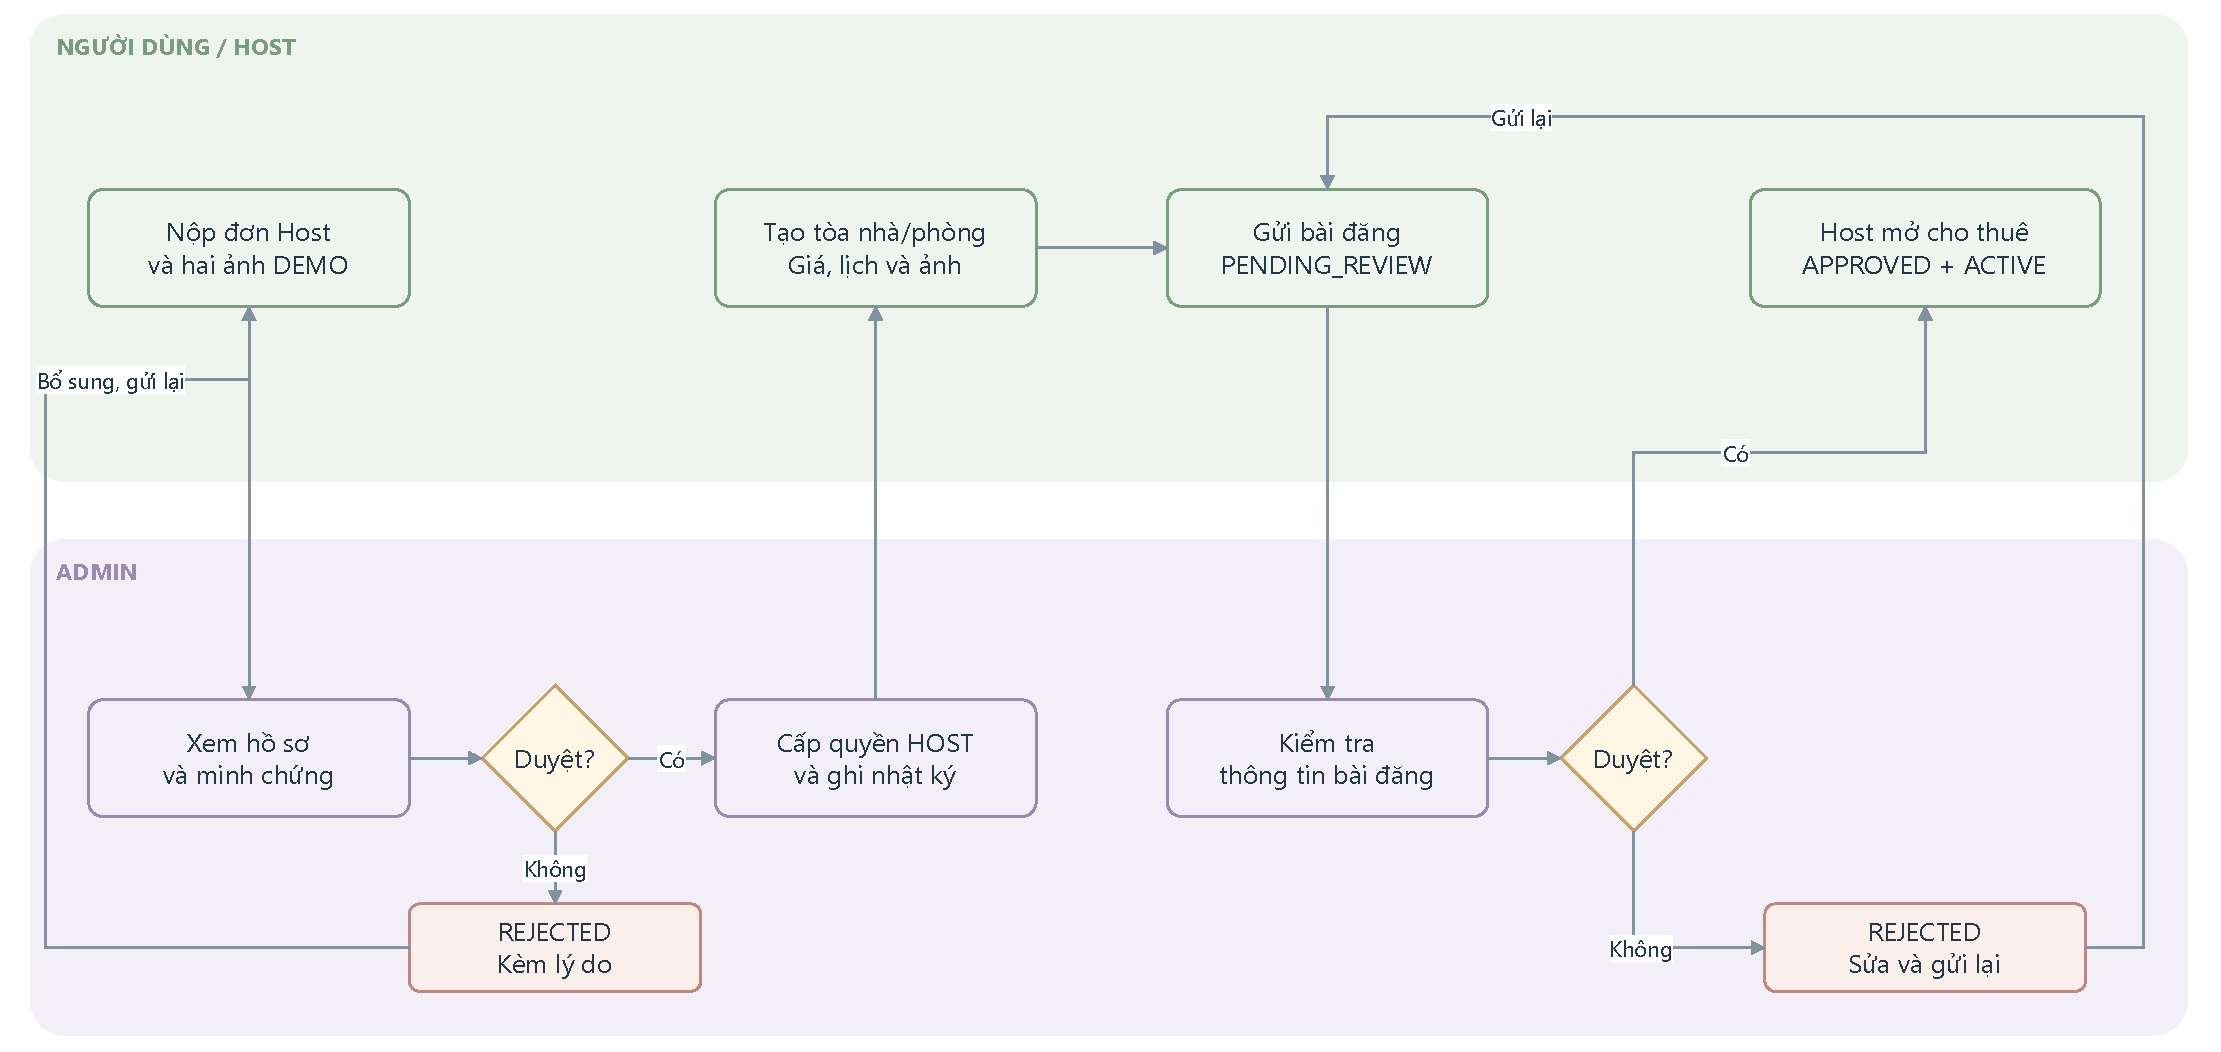
\includegraphics[page=1,width=\linewidth,height=0.82\textheight,keepaspectratio]{chapter2/workflow_diagram_v2.pdf}
\caption{Quy trình cấp quyền Host và công bố không gian.}\label{fig:app-host-workflow}
\end{figure}
\clearpage\BroomLandscapePagefalse\end{landscape}\pagestyle{fancy}
\clearpage
\begin{landscape}\pagestyle{empty}\BroomLandscapePagetrue
\begin{figure}[p]\centering
\includegraphics[page=2,width=\linewidth,height=0.82\textheight,keepaspectratio]{chapter2/workflow_diagram_v2.pdf}
\caption{Quy trình tạo, giữ lịch và xử lý yêu cầu đặt chỗ.}\label{fig:ch2-booking-workflow}
\end{figure}
\clearpage\BroomLandscapePagefalse\end{landscape}\pagestyle{fancy}
\clearpage
\begin{landscape}\pagestyle{empty}\BroomLandscapePagetrue
\begin{figure}[p]\centering
\includegraphics[page=3,width=\linewidth,height=0.82\textheight,keepaspectratio]{chapter2/workflow_diagram_v2.pdf}
\caption{Quy trình sử dụng phòng, khép lượt thuê và xác minh ngoại lệ.}\label{fig:app-usage-workflow}
\end{figure}
\clearpage\BroomLandscapePagefalse\end{landscape}\pagestyle{fancy}
\clearpage
\begin{landscape}\pagestyle{empty}\BroomLandscapePagetrue
\begin{figure}[p]\centering
\includegraphics[page=4,width=\linewidth,height=0.82\textheight,keepaspectratio]{chapter2/workflow_diagram_v2.pdf}
\caption{Luồng tạo QR và cập nhật kết quả thanh toán payOS.}\label{fig:app-payment-workflow}
\end{figure}
\clearpage\BroomLandscapePagefalse\end{landscape}\pagestyle{fancy}

\subsection{Sơ đồ phân rã chức năng}
Các chức năng được phân rã từ mục tiêu của từng vai trò đến nhóm thao tác liên quan. Nhóm người thuê bao gồm tài khoản, khám phá, booking, tương tác và hồ sơ Host; nhóm Host tập trung vào phòng, lịch và vận hành lượt thuê; nhóm Admin tập trung vào xét duyệt, xử lý vi phạm và kiểm tra nghiệp vụ. Cách phân rã tại Hình~\ref{fig:ch2-functions} làm rõ trách nhiệm mà không đồng nhất mỗi màn hình với một chức năng độc lập.

\begin{figure}[H]\centering
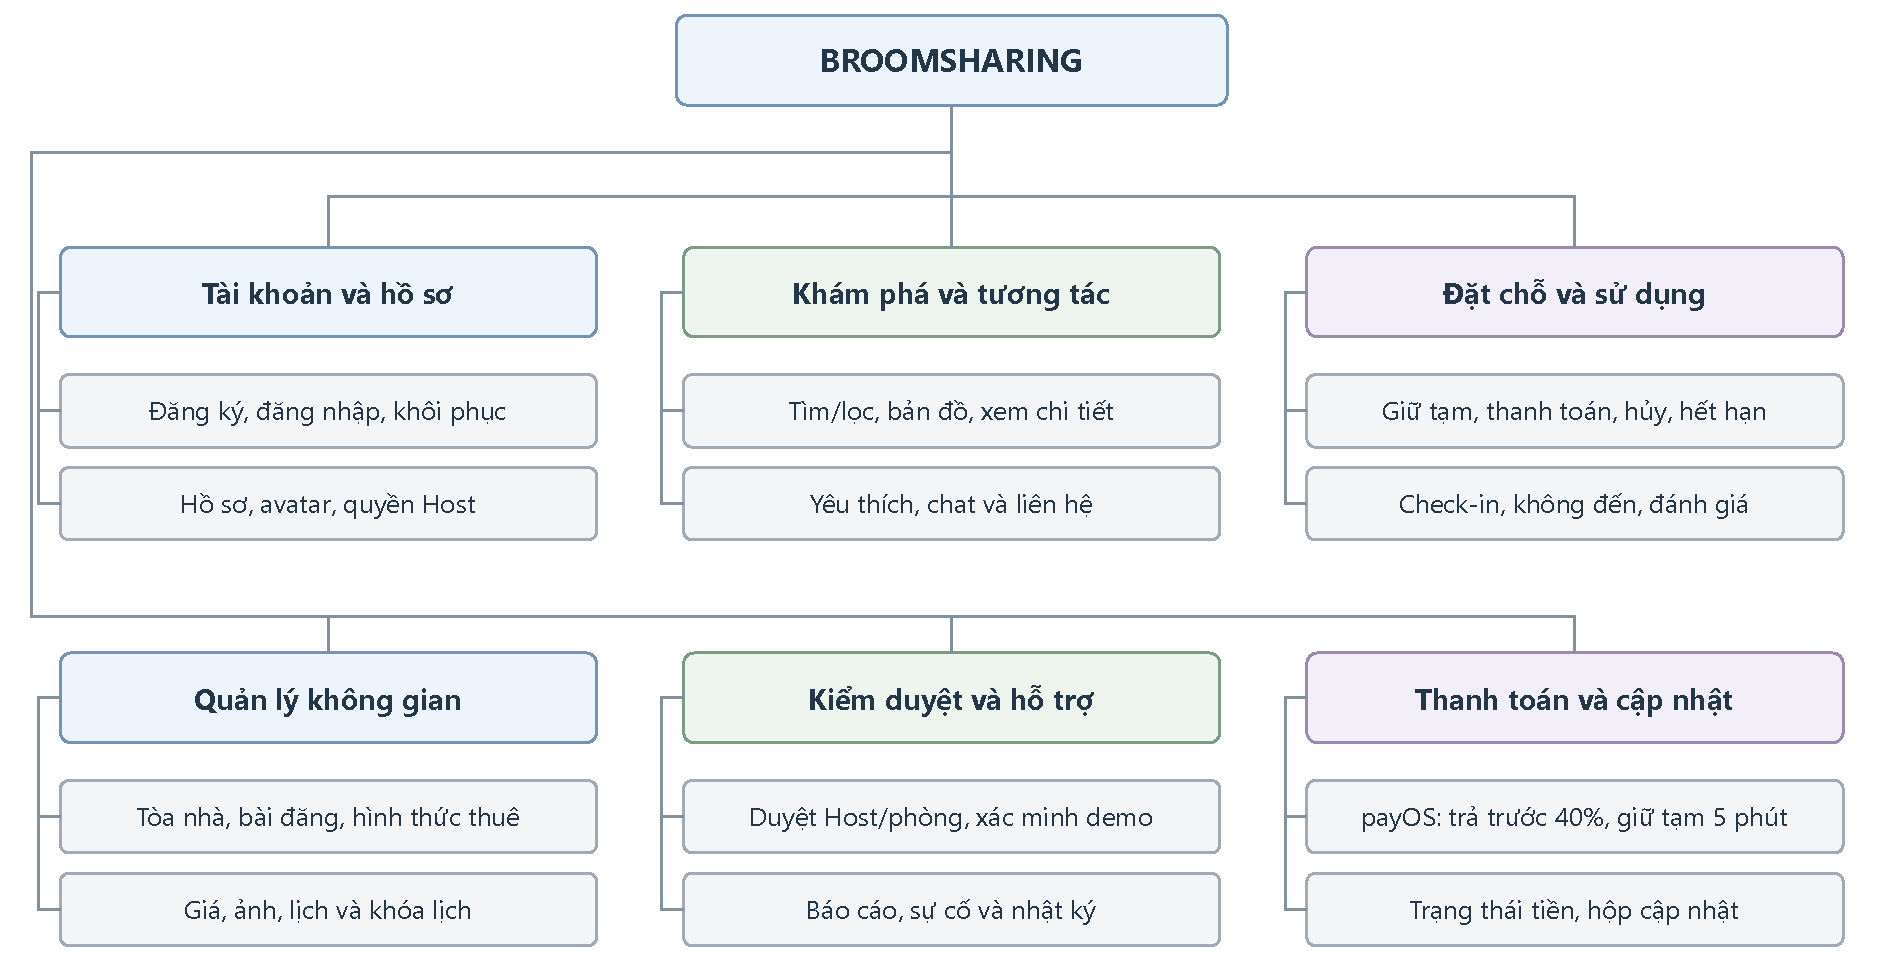
\includegraphics[page=1,width=\textwidth]{chapter2/usecase_decomposition_v2.pdf}
\caption{Phân rã chức năng tổng quát của BroomSharing.}\label{fig:ch2-functions}
\end{figure}

Chức năng tin nhắn hỗ trợ trao đổi giữa hai bên của một hội thoại. Hộp cập nhật tổng hợp sự kiện booking và trạng thái đã đọc của từng tài khoản. Đánh giá gắn với lượt đã sử dụng, còn báo cáo vi phạm được chuyển đến Admin và cho phép Host phản hồi. Các chức năng này bổ sung thông tin xử lý cho lượt thuê, đồng thời duy trì giới hạn truy cập theo vai trò và chủ thể liên quan.

Các nhánh phân rã theo từng nhóm được trình bày tại \hyperref[app:chapter2-details]{Phụ lục G}.

\subsection{Sơ đồ use case}
Hình~\ref{fig:ch2-usecase-overview} mô tả các mục tiêu tương tác với hệ thống. Host kế thừa khả năng thuê phòng của người thuê và có thêm nhóm chức năng cho thuê. Admin có tuyến chức năng kiểm duyệt riêng; quyền quản trị không mặc định bao gồm đọc hội thoại riêng của người dùng.

\begin{figure}[H]\centering
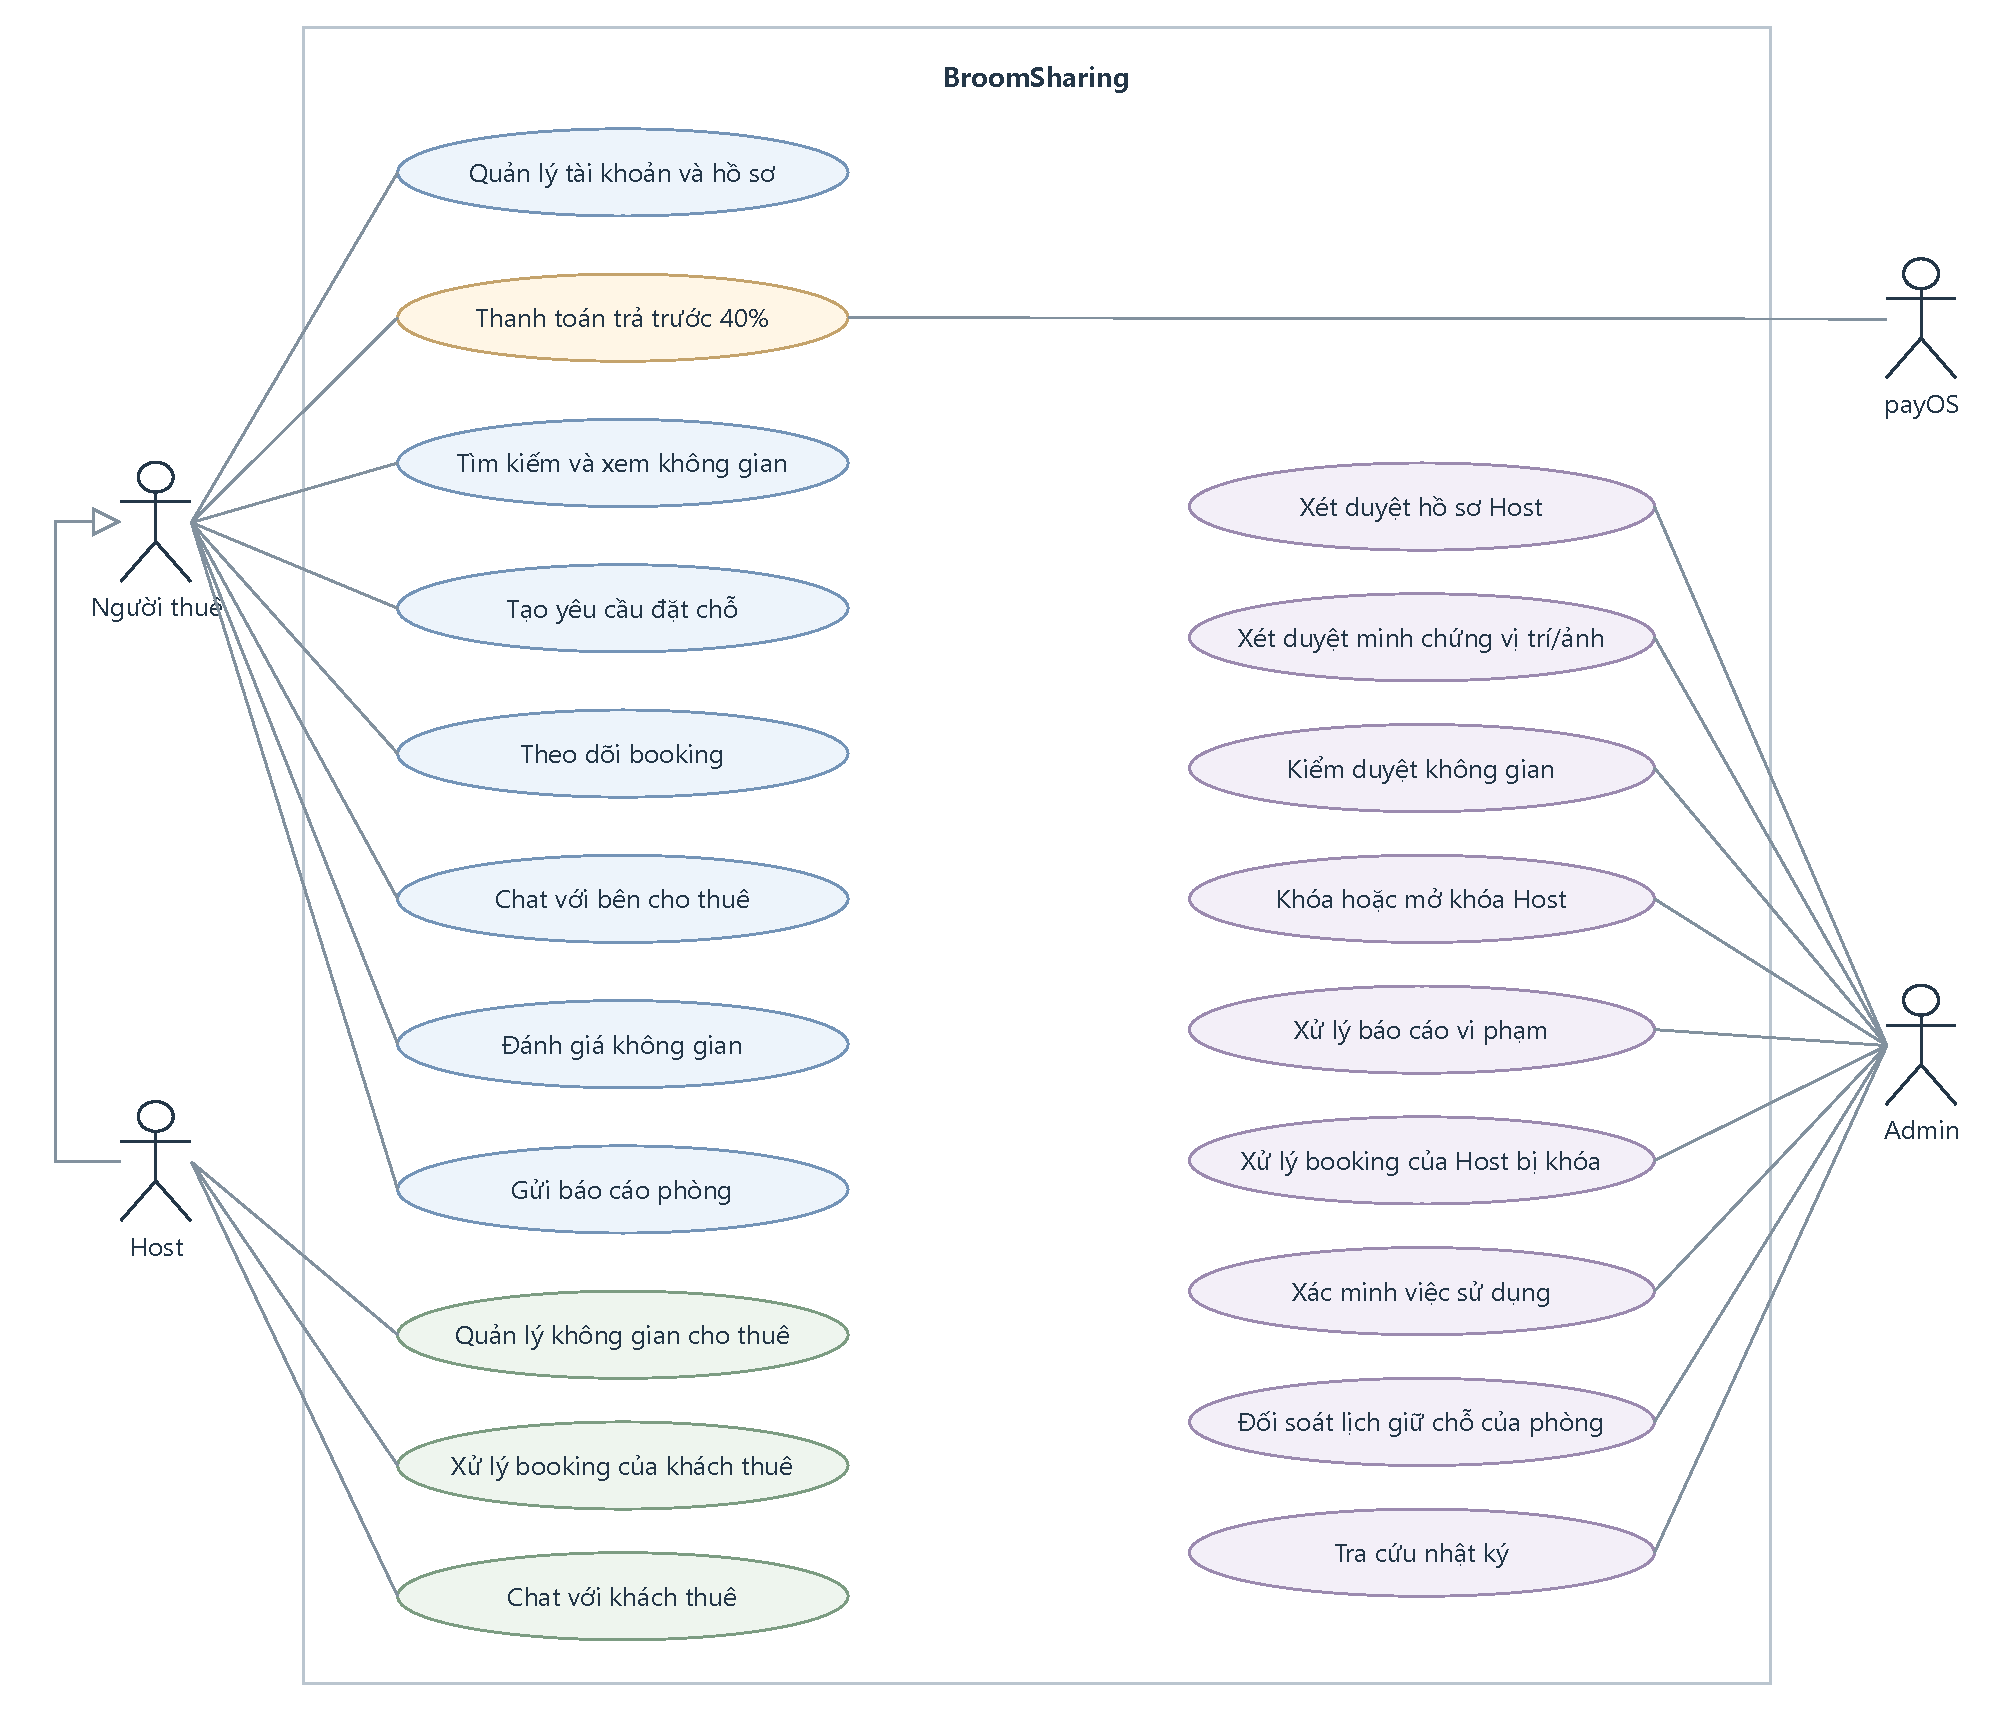
\includegraphics[page=1,width=0.95\textwidth]{chapter2/usecase_diagram_v2.pdf}
\caption{Use case tổng quát với các tác nhân người thuê, Host, Admin và dịch vụ thanh toán.}\label{fig:ch2-usecase-overview}
\end{figure}

Ở phân hệ người thuê, đặt chỗ luôn bao gồm kiểm tra khả dụng và mở bước thanh toán, còn hủy booking là thao tác có điều kiện trên lượt đang được theo dõi. Gửi đơn làm Host bao gồm cung cấp hai ảnh DEMO. Các phân hệ Host và Admin giữ liên kết tác nhân với mục tiêu nghiệp vụ; những cập nhật lịch và nhật ký được mô tả trong quy trình xử lý. Hình~\ref{fig:app-usecase-guest}, Hình~\ref{fig:app-usecase-host} và Hình~\ref{fig:app-usecase-admin} trình bày chi tiết mục tiêu của từng phân hệ.


\clearpage
Phân hệ người thuê bao quát truy cập tài khoản, khám phá, đặt chỗ và tương tác sau thuê. Kiểm tra khả dụng và mở thanh toán thuộc thao tác đặt chỗ; hủy booking chỉ thực hiện khi lượt thuê còn đáp ứng điều kiện hủy.
\begin{figure}[H]\centering
\includegraphics[page=2,width=\textwidth,height=0.75\textheight,keepaspectratio]{chapter2/usecase_diagram_v2.pdf}
\caption{Use case chi tiết của người thuê.}\label{fig:app-usecase-guest}
\end{figure}
\clearpage
Host quản lý tòa nhà, phòng, giá và lịch, đồng thời ghi nhận việc sử dụng và các ngoại lệ của lượt thuê. Quyền thuê dùng chung được kế thừa tại sơ đồ tổng quát; trang này tập trung vào các mục tiêu cho thuê.
\begin{figure}[H]\centering
\includegraphics[page=3,width=\textwidth,height=0.80\textheight,keepaspectratio]{chapter2/usecase_diagram_v2.pdf}
\caption{Use case chi tiết của Host.}\label{fig:app-usecase-host}
\end{figure}
\clearpage
Admin xét duyệt hồ sơ, bài đăng và minh chứng, xử lý vi phạm và can thiệp các booking thuộc phạm vi quản trị. Xác minh việc sử dụng và đối soát lịch được tách thành các mục tiêu riêng để phản ánh điều kiện xử lý khác nhau.
\begin{figure}[H]\centering
\includegraphics[page=4,width=\textwidth,height=0.80\textheight,keepaspectratio]{chapter2/usecase_diagram_v2.pdf}
\caption{Use case chi tiết của Admin.}\label{fig:app-usecase-admin}
\end{figure}

\subsection{Đặc tả các nghiệp vụ tiêu biểu}
\subsubsection{Gửi yêu cầu đặt chỗ}
Mục tiêu của nghiệp vụ là tạo lượt thuê có giá và quyền giữ lịch xác định. Điều kiện đầu vào gồm tài khoản được phép thuê, phòng đã duyệt và hoạt động, Host hợp lệ và thời gian chưa bắt đầu; không được đặt phòng của chính mình. Với thuê theo giờ, khoảng chọn phải đáp ứng ngày làm việc, giờ mở cửa và thời lượng tối thiểu. Cả hai chế độ đều được kiểm tra khoảng khóa liên quan.

Với thuê theo giờ, ứng dụng xác định các slot kỹ thuật 30 phút cần giữ trong khoảng được chọn; với thuê cố định, yêu cầu giữ toàn bộ một hoặc ba tháng. Hai chế độ không được dùng đồng thời cho cùng phòng. Mức giá dự kiến trên giao diện chỉ phục vụ xác nhận lựa chọn; trước khi tạo booking, dữ liệu phòng và lịch tiếp tục được kiểm tra trong transaction. Kết quả thành công là booking \texttt{PENDING} cùng các khóa lịch tương ứng, chưa phải booking đã thanh toán thành công. Màn hình tiếp theo mở QR; backend mới có quyền xác nhận kết quả nhận tiền.

Nhánh không thành công phân biệt dữ liệu nhập không phù hợp với lịch vừa bị người khác giữ. Nếu hai tài khoản gửi yêu cầu trùng nhau, chỉ yêu cầu còn thỏa điều kiện khi ghi dữ liệu được chấp nhận. Khi gửi lại cùng định danh yêu cầu và cùng nội dung, Repository trả về booking đã có thay vì tạo thêm bản ghi. Cách xử lý này tránh tạo lặp khi kết quả phản hồi chậm hoặc người dùng gửi lại thao tác.

\subsubsection{Điều kiện xử lý và khép lượt thuê}
Mỗi thao tác phải kiểm tra trạng thái hiện tại và quyền của người thực hiện, kể cả khi nút xử lý đã được hiển thị trước đó. Đối với hủy thông thường, booking phải còn ở trạng thái cho phép và chưa tới giờ bắt đầu; Host phải cung cấp lý do. Kết quả được lưu cùng người xử lý và mốc thời gian để các bên nhận biết nguồn gốc thay đổi.

Khi khép lượt, hệ thống giải phóng đúng lịch do booking đó giữ và bảo toàn lịch sử. Nếu Admin bổ sung xác nhận sử dụng hoặc sửa kết luận không đến, thao tác chỉ cập nhật kết quả liên quan, không nhả lịch lần thứ hai. Quyền đánh giá được kiểm tra từ người thuê, trạng thái đã khép và xác nhận sử dụng, thay vì chỉ dựa vào việc thời gian thuê đã kết thúc.

\subsubsection{Báo cáo vi phạm và xử lý quản trị}
Người thuê gửi báo cáo đối với phòng, mô tả vấn đề cần giải quyết; Host có thể phản hồi khi báo cáo còn mở. Admin xem thông tin đối tượng cùng phản hồi trước khi giải quyết hoặc bác báo cáo. Nếu cần hạn chế hoạt động, Admin có thể đình chỉ phòng hoặc khóa Host trong phạm vi thao tác được hỗ trợ. Báo cáo là hồ sơ xử lý vi phạm, không thay thế đánh giá của khách về một lượt sử dụng.

Đình chỉ phòng làm thay đổi khả năng nhận yêu cầu mới, nhưng không xóa lịch sử booking. Với Host bị khóa, các lượt chưa khép phải được xem xét từng trường hợp theo quy trình ngoại lệ. Việc gỡ đình chỉ cũng không tự mở phòng trở lại cho thuê: phòng chuyển về không hoạt động để Host chủ động kiểm tra trước khi công bố. Cách tách các quyết định này giúp tránh một thao tác quản trị làm thay đổi ngoài ý muốn toàn bộ vòng đời của các lượt thuê liên quan.

\subsection{Yêu cầu phi chức năng và các ràng buộc thiết kế}
Về tính nhất quán, một phòng chỉ được giữ độc quyền trong khoảng thuê, kể cả trong thời hạn tạm giữ chờ thanh toán. Các thay đổi booking, lịch và thông tin kiểm soát của phòng phải cùng thành công hoặc cùng bị từ chối trong thao tác tương ứng. Lịch không được chỉnh bằng cách chỉ ẩn một booking trên giao diện; các khóa đang giữ phải được giải phóng theo chính bản ghi đã tạo chúng.

Về phân quyền, ứng dụng kiểm tra cả vai trò và quan hệ với đối tượng. Host chỉ quản lý tài sản thuộc sở hữu; người thuê chỉ thực hiện quyền của mình trên booking; thành viên hội thoại mới được đọc và gửi tin trong hội thoại đó. Firestore Security Rules cho phép kiểm tra danh tính và dữ liệu trong điều kiện cho phép hoặc từ chối thao tác \parencite{firebase_rules_conditions}. Backend thanh toán sử dụng thông tin xác thực và kiểm tra nghiệp vụ phía máy chủ, không lấy số tiền do màn hình tự khai báo làm căn cứ thu tiền.

Về khả năng sử dụng, giao diện phân biệt đang tải, danh sách trống, lỗi và kết quả thành công. Khi dữ liệu thay đổi từ tài khoản khác, màn hình cần cập nhật trạng thái và kiểm tra lại trước thao tác quan trọng. Lỗi kết nối phải có phản hồi và cho phép thử lại khi phù hợp, đồng thời tránh tạo lặp dữ liệu. Các yêu cầu này được đánh giá qua kịch bản thao tác trên thiết bị và kết nối cụ thể.

\chapstart
\section{THIẾT KẾ GIAO DIỆN}
\subsection{Tổng quan về thiết kế giao diện}
Giao diện BroomSharing sử dụng xanh lục, xanh ngọc làm điểm nhấn trên nền trắng và xám nhẹ. Các màn hình thống nhất cách bố trí tiêu đề, trường nhập, thẻ thông tin và nút thao tác chính để làm nổi bật nội dung không gian.

Danh sách phòng sử dụng \texttt{RecyclerView} để tái sử dụng các View khi hiển thị dữ liệu \parencite{android_recycler}. Thanh điều hướng người thuê gồm Trang chủ, Bản đồ, Lượt thuê, Tin nhắn và Cá nhân; Host và Admin có khu vực quản lý riêng.

Bộ hình trong chương là prototype ban đầu do nhóm xây dựng trên Figma, thể hiện bố cục và hướng tương tác dự kiến. Các màn hình đặt trọng tâm vào trình tự sử dụng và cách nhóm thông tin; giao diện hiện thực cùng kết quả kiểm thử được trình bày ở các chương sau. Những lựa chọn xuất hiện trong prototype vì vậy được xem xét ở mức phương án thiết kế, không đồng nhất với toàn bộ chức năng đã tích hợp.

\subsubsection{Phân cấp thông tin và hành động}
Các màn hình tìm thuê được tổ chức theo mức độ cần thiết của thông tin. Trang chủ ưu tiên ảnh, loại không gian và giá để hỗ trợ so sánh; chi tiết phòng bổ sung điều kiện sử dụng và vị trí; bước xác nhận tập hợp thời gian, liên hệ và chi phí trước khi gửi yêu cầu. Dữ liệu được mở dần theo tiến trình, tránh đặt toàn bộ nội dung của phòng lên thẻ danh sách.

Hành động chính sử dụng màu nhấn và tên gắn với mục tiêu như đăng nhập, thuê ngay hoặc gửi yêu cầu. Những thao tác phụ như xem lại, thay đổi thông tin và quay về được đặt gần khối liên quan. Đối với hủy, từ chối hoặc khóa đối tượng, thiết kế cần thể hiện rõ đích tác động và bước xác nhận, vì các thao tác này làm thay đổi quyền sử dụng hoặc trạng thái xử lý.

\subsubsection{Trạng thái giao diện và tính nhất quán}
Thiết kế phân biệt đang tải, dữ liệu trống, dữ liệu không hợp lệ và kết quả gửi. Danh sách chưa tải xong không được thể hiện như không có kết quả; nút đã nhấn cũng chưa phải xác nhận lưu thành công. Khi gửi biểu mẫu, trạng thái xử lý giúp hạn chế thao tác lặp. Nếu có lỗi, thông báo gắn với nội dung cần sửa và giữ lại phần dữ liệu còn phù hợp. Các phản hồi này là yêu cầu cho bản hiện thực từ prototype.

\clearpage

\subsection{Giao diện phân hệ người thuê}
\subsubsection{Đăng nhập và đăng ký}
Giao diện đăng nhập gồm tài khoản, mật khẩu và đường dẫn đến đăng ký, quên mật khẩu. Màn hình đăng ký thu thập họ tên, thông tin liên hệ, mật khẩu và xác nhận mật khẩu. Các trường sắp theo thứ tự nhập, với điều khoản sử dụng đặt trước nút hoàn tất.

Hình~\ref{fig:ch3-auth} phân nhóm trường nhập và làm nổi bật nút đăng nhập, đăng ký. Biểu tượng mật khẩu hỗ trợ kiểm tra nội dung nhập; lựa chọn Google/Zalo đặt ở vùng riêng để phân biệt với biểu mẫu tài khoản của ứng dụng.

Khi biểu mẫu có lỗi, phản hồi cần phân biệt thiếu dữ liệu, thông tin chưa đúng định dạng và xác thực không thành công. Nội dung mật khẩu được che mặc định; dữ liệu còn hợp lệ không bị xóa chỉ vì một trường khác cần sửa. Liên kết giữa đăng nhập và đăng ký giữ vai trò điều hướng, không làm người dùng nhầm với nút gửi biểu mẫu hiện tại.

\begin{figure}[H]\centering
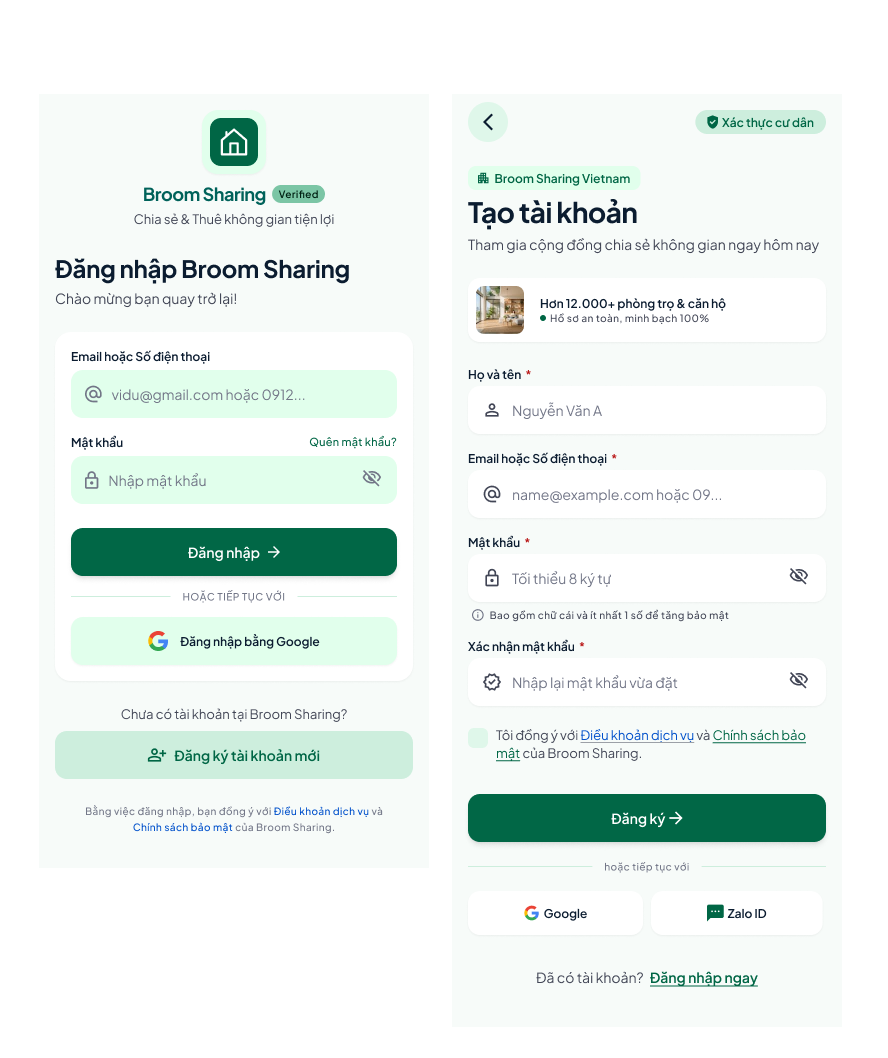
\includegraphics[width=0.9\textwidth,height=0.55\textheight,keepaspectratio]{chapter3/auth-design.png}
\caption{Thiết kế biểu mẫu đăng nhập và đăng ký tài khoản.}\label{fig:ch3-auth}
\end{figure}
\clearpage

\subsubsection{Trang chủ và chi tiết không gian}
Giao diện Trang chủ tích hợp thanh tìm kiếm, phân loại danh mục và danh sách không gian dưới dạng thẻ. Mỗi thẻ tập trung vào ảnh, tên phòng, khu vực, sức chứa và giá thuê. Hình~\ref{fig:ch3-home} minh họa thứ bậc hiển thị này qua hai vùng đối tác ưu tiên và không gian gợi ý. Thanh điều hướng đáy giữ các điểm truy cập chính ở vị trí ổn định khi duyệt danh sách.

Người dùng có thể tiếp cận bộ lọc từ vùng tìm kiếm và mở phòng cần xem. Màn hình chi tiết tại Hình~\ref{fig:ch3-detail} bổ sung bộ ảnh, diện tích, sức chứa, tiện ích, vị trí và thông tin Host. Nội dung dài được chia thành các khối để thuận tiện cuộn xem. Các hành động yêu thích, nhắn tin, chỉ đường và đặt thuê được bố trí gần thông tin liên quan để giảm thao tác chuyển màn hình.

Đơn vị giá cần đặt sát con số để phân biệt giá theo giờ với giá của kỳ thuê cố định. Các nhãn trạng thái và thông tin tiện ích giúp bổ sung ngữ cảnh, nhưng không thay thế phần điều kiện sử dụng trong chi tiết. Khi chuyển từ danh sách sang bản đồ hoặc mở phòng, lựa chọn phải tiếp tục trỏ đến cùng phòng để tránh nhầm đối tượng trước khi đặt.

\begin{figure}[H]\centering
\begin{minipage}[t]{0.31\textwidth}\centering
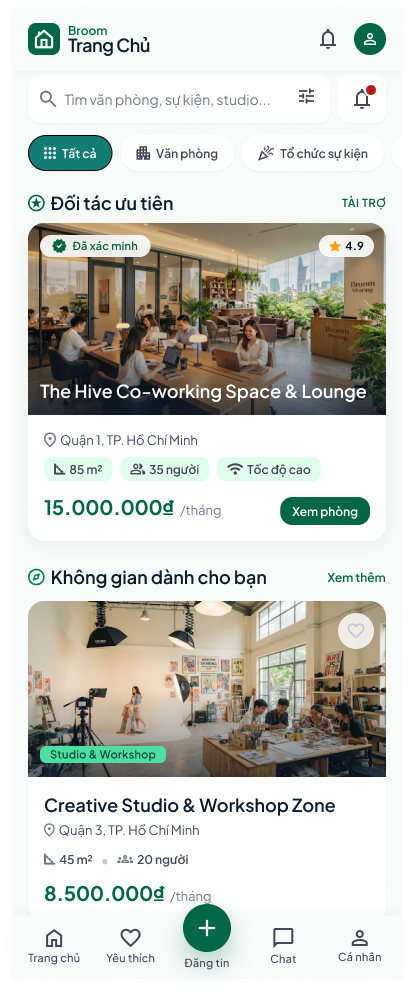
\includegraphics[width=\linewidth,height=0.47\textheight,keepaspectratio]{chapter3/home-design.png}
\caption{Thiết kế Trang chủ.}\label{fig:ch3-home}
\end{minipage}\hfill
\begin{minipage}[t]{0.65\textwidth}\centering
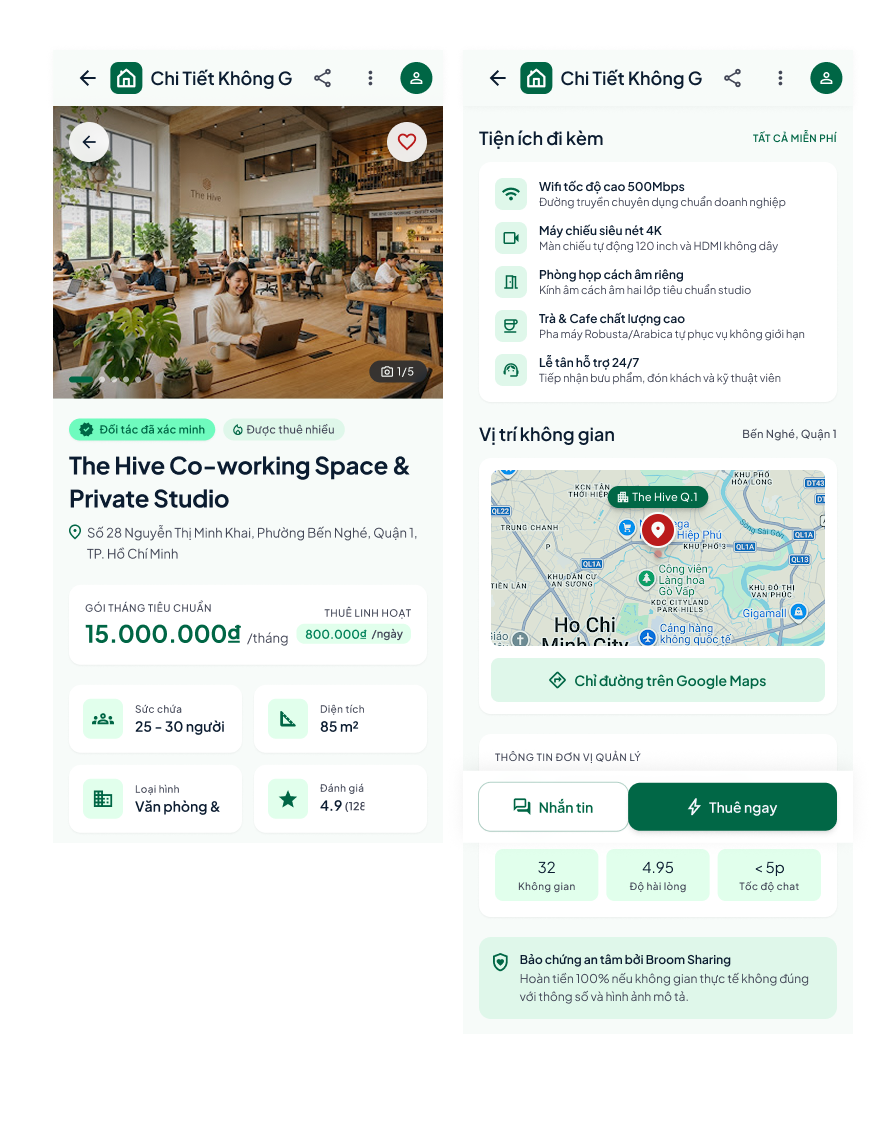
\includegraphics[trim=0 88 0 0,clip,width=\linewidth,height=0.47\textheight,keepaspectratio]{chapter3/detail-design.png}
\caption{Thiết kế thông tin chi tiết không gian.}\label{fig:ch3-detail}
\end{minipage}
\end{figure}

\clearpage
\subsubsection{Đặt chỗ, theo dõi và thanh toán}
Màn hình đặt chỗ tập hợp thời gian sử dụng, thông tin người thuê và giá dự kiến trước khi gửi yêu cầu. Khối thông tin phòng được giữ ở đầu màn hình để người dùng đối chiếu lựa chọn; vùng thời gian và liên hệ đặt ngay bên dưới. Đối với thiết kế nghiệp vụ, bộ chọn thời gian cần thích ứng với chế độ theo giờ hoặc kỳ thuê một, ba tháng của phòng.

Danh sách lượt thuê hiển thị thời gian, trạng thái booking và các thao tác còn hiệu lực. Phương án xác nhận tại Hình~\ref{fig:app-booking-design} tiếp tục chia nội dung thành hình thức thanh toán, thông tin hợp đồng và bảng chi phí. Tổng tiền cùng nút gửi yêu cầu nằm cuối tiến trình để người dùng kiểm tra trước khi xác nhận. Khi hiện thực luồng thanh toán, thông tin tiền cần tách khỏi trạng thái nhận phòng và hoàn tất.

Ở bước xác nhận, thay đổi kỳ thuê phải dẫn đến cập nhật phần thời gian và chi phí liên quan. Thiết kế dành vị trí cho thông tin người thuê, cho phép đối chiếu liên hệ mà không phải quay về hồ sơ để xem lại. Các nhãn bảo chứng, lựa chọn hợp đồng và số tiền cụ thể trong hình là nội dung minh họa của phương án ban đầu; thiết kế chi tiết khi triển khai phải bám chính sách đã xác định ở Chương 2.

\begin{figure}[H]\centering
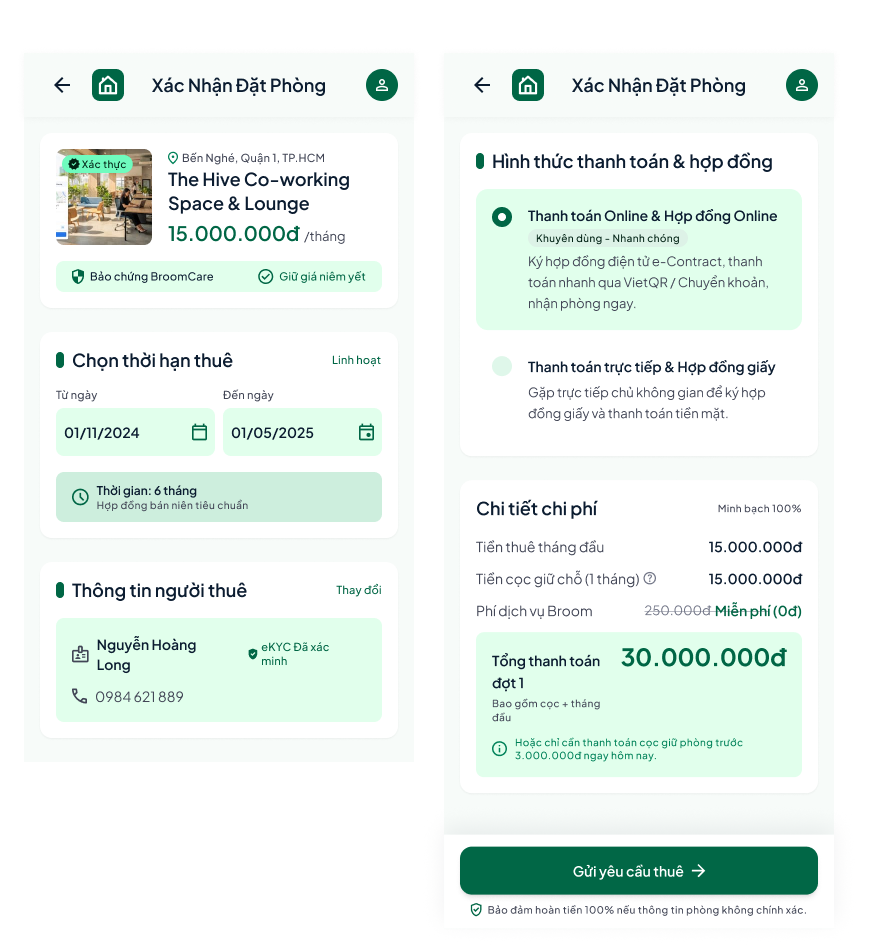
\includegraphics[width=\textwidth,height=0.48\textheight,keepaspectratio]{chapter3/booking-design.png}
\caption{Prototype xác nhận thông tin và chi phí đặt phòng.}\label{fig:app-booking-design}
\end{figure}

\clearpage
\subsubsection{Hồ sơ và tương tác}
Giao diện Cá nhân phân nhóm hồ sơ, ảnh đại diện, phòng yêu thích, lịch sử và đăng ký quyền Host. Khu vực tin nhắn tổ chức hội thoại với chủ không gian; hộp cập nhật tập trung sự kiện liên quan đến lượt thuê và trạng thái đã đọc.

Biểu mẫu đánh giá gồm điểm và nhận xét, chỉ mở sau lượt thuê đã xác nhận sử dụng và khép lại. Báo cáo vi phạm có nội dung riêng gửi Admin, tách khỏi nhận xét công khai về phòng.

Đối với hội thoại, danh sách cần thể hiện người trao đổi, nội dung gần nhất và tình trạng đã đọc; màn hình chat giữ ngữ cảnh phòng để hỗ trợ trao đổi. Thông tin chưa đọc phục vụ việc nhận biết thay đổi, không làm phát sinh một trạng thái mới của booking. Các đường dẫn từ thông báo hoặc hội thoại phải mở đúng đối tượng liên quan thay vì chỉ đưa về Trang chủ.

\subsection{Giao diện phân hệ chủ không gian}
Giao diện Host tập trung vào phòng, booking và lịch hoạt động. Khi đăng phòng, biểu mẫu phân nhóm thông tin cơ bản, giá và lịch, hình ảnh và điều kiện sử dụng. Hình~\ref{fig:ch3-host} minh họa cách giữ các trường cùng mục đích gần nhau trong ba bước nhập liệu.

Thông tin cơ bản gồm vị trí, loại không gian, diện tích và sức chứa. Phần giá và lịch tuân theo chế độ thuê của phòng; phần hình ảnh tập trung ảnh, mô tả và tiện ích. Thanh tiến trình cùng nút tiếp tục, quay lại giúp nhận biết bước hiện tại và kiểm tra thông tin trước khi gửi bài.

Tại màn hình booking, các thao tác của Host được phân biệt theo trạng thái: xác nhận, từ chối, hủy, nhận phòng, hoàn tất hoặc ghi nhận khách không đến. Những thao tác cần giải trình có ô nhập lý do. Màn hình lịch và danh sách phòng bổ sung góc nhìn tổng hợp về khoảng đã giữ, trạng thái bài đăng và yêu cầu cần xử lý.

Khi đăng tin theo nhiều bước, thông tin đã nhập cần được giữ trong quá trình đi tới hoặc quay lại giữa các bước của biểu mẫu. Vùng ảnh cần phân biệt ảnh đã chọn, đang tải và tải lỗi trước khi gửi bài. Đối với quản lý phòng, trạng thái chờ duyệt và trạng thái tạm ngừng không được thể hiện bằng cùng một nhãn, vì chúng có nguyên nhân và hành động tiếp theo khác nhau.

\begin{figure}[H]\centering
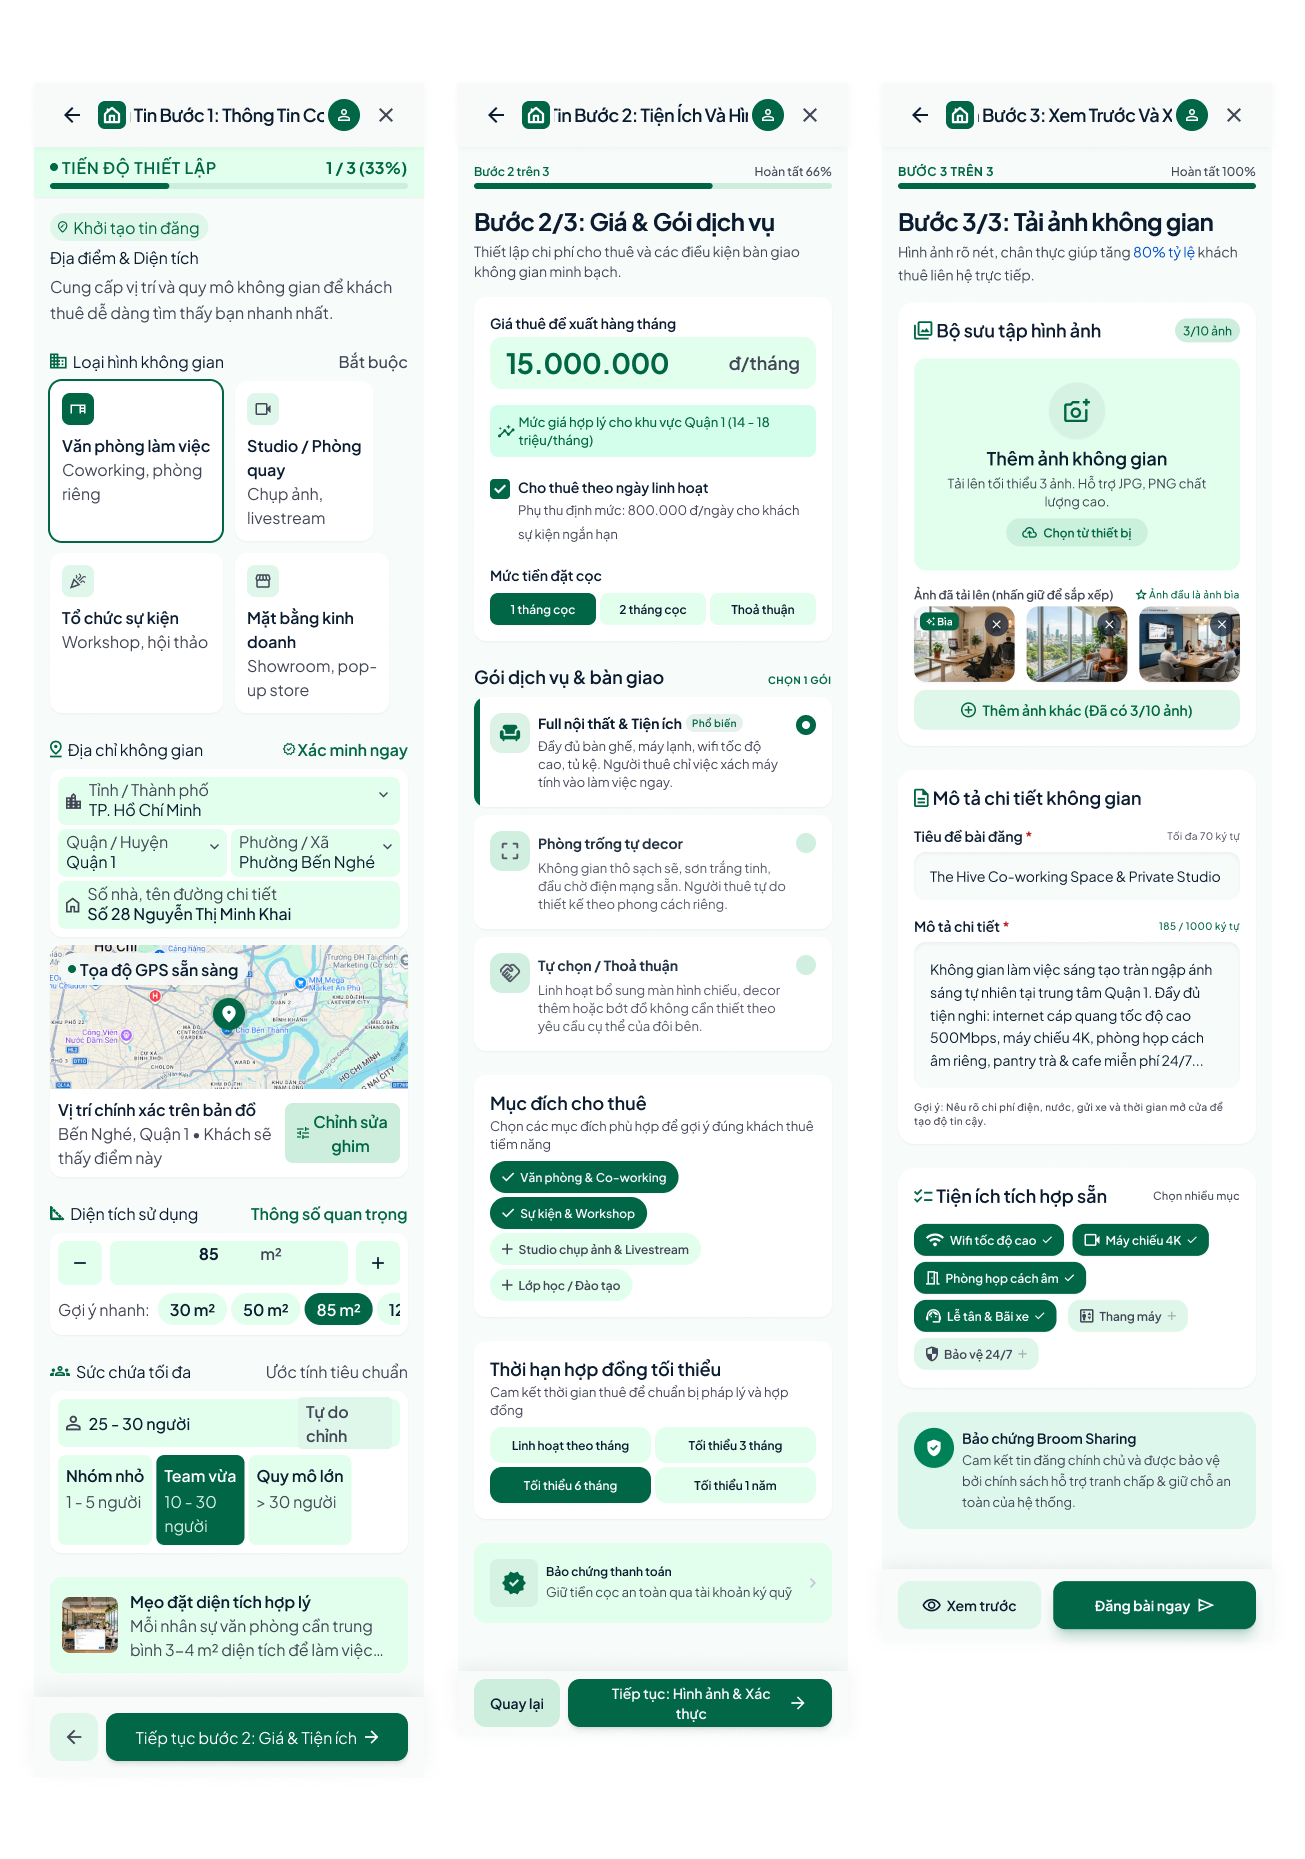
\includegraphics[width=\textwidth,height=0.5\textheight,keepaspectratio]{chapter3/host-design.png}
\caption{Prototype ba bước nhập thông tin và đăng không gian.}\label{fig:ch3-host}
\end{figure}

\subsection{Giao diện phân hệ quản trị viên}
Giao diện Admin phân chia khu vực tổng quan, xét duyệt, quản lý và báo cáo. Hồ sơ, bài đăng được hiển thị cùng trạng thái và mở chi tiết trước khi chấp thuận hoặc từ chối. Đơn xin quyền Host và minh chứng vị trí/hình ảnh là các nhóm độc lập.

Hình~\ref{fig:app-admin-design} đặt bộ lọc phía trên danh sách, gắn nút phê duyệt hoặc từ chối với hồ sơ đang xem. Trạng thái và lý do xử lý phân biệt khóa Host, đình chỉ phòng và khép booking. Các con số trong prototype phục vụ minh họa bố cục.

Trong thiết kế, danh sách cung cấp thông tin nhận diện nhanh, còn quyết định xử lý gắn với hồ sơ cụ thể. Trường hợp từ chối hoặc áp dụng hạn chế cần có vùng nhập lý do và xác nhận hành động. Hai nhóm kiểm duyệt phòng và quản lý tài khoản được bố trí riêng để phân biệt đối tượng chịu tác động; prototype đầy đủ được trình bày tại Phụ lục A.


\chapstart
\section{THIẾT KẾ CƠ SỞ DỮ LIỆU}
\label{sec:database-design}
\begingroup
\setlist[itemize]{leftmargin=1.27cm,label=\textbullet,itemsep=2pt,topsep=4pt}
\setlist[enumerate]{leftmargin=1.27cm,itemsep=2pt,topsep=4pt}
\setlength{\emergencystretch}{1em}
\widowpenalty=10000
\clubpenalty=10000

BroomSharing sử dụng database \texttt{broomsharing} của Cloud Firestore để lưu dữ liệu tài khoản, không gian, đặt chỗ và trao đổi giữa các bên. Firebase Authentication quản lý danh tính đăng nhập, liên kết với hồ sơ người dùng qua UID. Cloudinary lưu ảnh và minh chứng DEMO, còn Firestore giữ URL tham chiếu. Backend Java quản lý giao dịch payOS và trạng thái tiền \parencite{broomsharing_source}.

\subsection{Các thực thể và thuộc tính}
\label{sec:ch4-entities}

Dữ liệu ứng dụng được tổ chức thành 17 collection gốc và ba loại subcollection, tương ứng 20 mẫu document đang được ứng dụng hoặc backend sử dụng trong Bảng~\ref{tab:ch4-entities-summary}. Các thuộc tính định danh liên kết tài khoản với tài sản và yêu cầu thuê; nhóm trạng thái chi phối việc công bố phòng, xét duyệt và chuyển bước đặt chỗ. Collection thông báo cũ chỉ còn contract trong Rules, không phải nguồn hộp cập nhật đang hoạt động. Document còn chứa dữ liệu nhúng dạng \texttt{map}, \texttt{array} và các mốc thời gian xử lý. Những trường như người duyệt hoặc thời điểm hủy chỉ phát sinh khi nghiệp vụ tương ứng được thực hiện.

\begingroup\small\setstretch{1.06}
\begin{longtable}{@{}>{\raggedright\arraybackslash}p{3.6cm}>{\raggedright\arraybackslash}p{3.75cm}>{\raggedright\arraybackslash}p{7.9cm}@{}}
\caption{Các mẫu document và thuộc tính tiêu biểu}\label{tab:ch4-entities-summary}\\
\toprule Đường dẫn & Vai trò & Thuộc tính tiêu biểu và kiểu \\ \midrule\endfirsthead
\toprule Đường dẫn & Vai trò & Thuộc tính tiêu biểu và kiểu \\ \midrule\endhead
\midrule\multicolumn{3}{r}{\small Còn tiếp ở trang sau}\\\endfoot
\bottomrule\endlastfoot
\texttt{users/\allowbreak{}\{\allowbreak{}uid\}} & Hồ sơ và quyền tài khoản. & \texttt{uid}, \texttt{role}, \texttt{status}, \texttt{photo\allowbreak{}Url} (\texttt{string}); \ldots \\
\texttt{public\allowbreak{}Hosts/\allowbreak{}\{\allowbreak{}uid\}} & Bản chiếu Host. & \texttt{uid}, \texttt{name}, \texttt{photo\allowbreak{}Url} (\texttt{string}); \ldots \\
\texttt{usernames/\allowbreak{}\{\allowbreak{}normalized\allowbreak{}Username\}} & Ánh xạ đăng nhập. & \texttt{uid}, \texttt{email} (\texttt{string}). \\
\texttt{host\allowbreak{}Applications/\allowbreak{}\{\allowbreak{}uid\}} & Đơn cấp quyền Host. & \texttt{applicant\allowbreak{}Uid}, \texttt{status} (\texttt{string}); \texttt{identity\allowbreak{}Image\allowbreak{}Urls} (\texttt{array\textless{}\allowbreak{}string\textgreater{}}); \ldots \\
\texttt{users/\allowbreak{}\{\allowbreak{}uid\}\allowbreak{}/\allowbreak{}favorites/\allowbreak{}\{\allowbreak{}room\allowbreak{}Id\}} & Phòng yêu thích. & \texttt{room\allowbreak{}Id}, \texttt{room\allowbreak{}Name} (\texttt{string}); \texttt{created\allowbreak{}At} (\texttt{timestamp}). \\
\texttt{users/\allowbreak{}\{\allowbreak{}uid\}\allowbreak{}/\allowbreak{}notice\allowbreak{}Reads/\allowbreak{}\{\allowbreak{}event\allowbreak{}Id\}} & Mốc đọc sự kiện dẫn xuất. & \texttt{read\allowbreak{}At} (\texttt{timestamp}). \\
\texttt{buildings/\allowbreak{}\{\allowbreak{}building\allowbreak{}Id\}} & Địa điểm và chủ sở hữu. & \texttt{owner\allowbreak{}Uid}, \texttt{name}, \texttt{address} (\texttt{string}); \texttt{location} (\texttt{geopoint/\allowbreak{}null}); \ldots \\
\texttt{rooms/\allowbreak{}\{\allowbreak{}room\allowbreak{}Id\}} & Không gian và trạng thái tin. & \texttt{building\allowbreak{}Id}, \texttt{owner\allowbreak{}Uid}, \texttt{active\allowbreak{}Mode} (\texttt{string}); \texttt{active\allowbreak{}Booking\allowbreak{}Count} (\texttt{integer}); \ldots \\
\texttt{bookings/\allowbreak{}\{\allowbreak{}booking\allowbreak{}Id\}} & Kỳ thuê, trạng thái và giá đã chốt. & \texttt{room\allowbreak{}Id}, \texttt{guest\allowbreak{}Uid}, \texttt{status}, \texttt{payment\allowbreak{}Flow} (\texttt{string}); \texttt{price\allowbreak{}Snapshot} (\texttt{map}); \ldots \\
\texttt{availability\allowbreak{}Months/\allowbreak{}\{\allowbreak{}room\allowbreak{}Id\_\allowbreak{}yyyy\allowbreak{}MM\}} & Khóa lịch chính thức và tạm giữ. & \texttt{fixed\allowbreak{}Booking\allowbreak{}Id} (\texttt{string}); \texttt{slots\allowbreak{}Busy} (\texttt{array\textless{}\allowbreak{}integer\textgreater{}}); \texttt{hourly\allowbreak{}Bookings} (\texttt{map\textless{}\allowbreak{}string,\allowbreak{}array\textless{}\allowbreak{}integer\textgreater{}\allowbreak{}\textgreater{}}); \texttt{pending\allowbreak{}Payment\allowbreak{}Ids} (\texttt{array\textless{}\allowbreak{}string\textgreater{}}); \ldots \\
\texttt{payments/\allowbreak{}\{\allowbreak{}booking\allowbreak{}Id\}} & Giao dịch trả trước. & \texttt{order\allowbreak{}Code}, \texttt{amount}, \texttt{expires\allowbreak{}At} (\texttt{integer}); \texttt{status} (\texttt{string}); \ldots \\
\texttt{payment\allowbreak{}Orders/\allowbreak{}\{\allowbreak{}order\allowbreak{}Code\}} & Ánh xạ mã đơn của backend. & \texttt{booking\allowbreak{}Id} (\texttt{string}). \\
\texttt{app\allowbreak{}Config/\allowbreak{}payments} & Cấu hình kênh demo công khai. & \texttt{flow}, \texttt{demo\allowbreak{}Host\allowbreak{}Uid} (\texttt{string}). \\
\texttt{reviews/\allowbreak{}\{\allowbreak{}booking\allowbreak{}Id\}} & Đánh giá sau sử dụng. & \texttt{room\allowbreak{}Id}, \texttt{guest\allowbreak{}Uid}, \texttt{comment} (\texttt{string}); \texttt{rating} (\texttt{integer}); \ldots \\
\texttt{conversations/\allowbreak{}\{\allowbreak{}guest\allowbreak{}Uid:host\allowbreak{}Uid\}} & Hội thoại và mốc đọc. & \texttt{member\allowbreak{}Uids} (\texttt{array\textless{}\allowbreak{}string\textgreater{}}); \texttt{sequence}, \texttt{guest\allowbreak{}Read}, \texttt{host\allowbreak{}Read} (\texttt{integer}); \ldots \\
\texttt{conversations/\allowbreak{}\{\allowbreak{}guest\allowbreak{}Uid:host\allowbreak{}Uid\}\allowbreak{}/\allowbreak{}messages/\allowbreak{}\{\allowbreak{}message\allowbreak{}Id\}} & Tin nhắn của hội thoại. & \texttt{sender\allowbreak{}Uid}, \texttt{text} (\texttt{string}); \texttt{sequence} (\texttt{integer}); \texttt{created\allowbreak{}At} (\texttt{timestamp}); \ldots \\
\texttt{property\allowbreak{}Verifications/\allowbreak{}\{\allowbreak{}verification\allowbreak{}Id\}} & Minh chứng xác minh. & \texttt{owner\allowbreak{}Uid}, \texttt{verification\allowbreak{}Type}, \texttt{status} (\texttt{string}); \texttt{evidence\allowbreak{}Refs} (\texttt{array\textless{}\allowbreak{}string\textgreater{}}); \ldots \\
\texttt{reports/\allowbreak{}\{\allowbreak{}report\allowbreak{}Id\}} & Phản ánh và kết quả xử lý. & \texttt{reporter\allowbreak{}Uid}, \texttt{room\allowbreak{}Id}, \texttt{booking\allowbreak{}Id}, \texttt{status} (\texttt{string}); \ldots \\
\texttt{audit\allowbreak{}Logs/\allowbreak{}\{\allowbreak{}audit\allowbreak{}Id\}} & Dấu vết thay đổi. & \texttt{actor\allowbreak{}Uid}, \texttt{target\allowbreak{}Path}, \texttt{action} (\texttt{string}); \texttt{before}, \texttt{after} (\texttt{map\textless{}\allowbreak{}string,\allowbreak{}any\textgreater{}}); \ldots \\
\texttt{rental\allowbreak{}Places/\allowbreak{}\{\allowbreak{}place\allowbreak{}Id\}} & Địa điểm tham khảo, không đặt thuê. & \texttt{name}, \texttt{source\allowbreak{}Url} (\texttt{string}); \texttt{location} (\texttt{geopoint}); \ldots \\
\end{longtable}\endgroup


Mô hình tách hồ sơ tài khoản khỏi bản chiếu Host, thông tin phòng khỏi lịch giữ chỗ và nội dung hội thoại khỏi từng tin nhắn. Các lớp tổng hợp phục vụ giao diện như \texttt{Room\allowbreak{}Listing}, \texttt{Booking\allowbreak{}Notice} và \texttt{Host\allowbreak{}Stats} không có collection độc lập. Trong booking, tên phòng, liên hệ người thuê và giá được lưu tại thời điểm đặt, duy trì ngữ cảnh của yêu cầu khi dữ liệu gốc thay đổi.

\subsection{Quan hệ dữ liệu và cấu trúc lưu trữ}
\label{sec:ch4-relationships}

Hình~\ref{fig:ch4-overview} thể hiện cây lưu trữ của hệ thống. Hai subcollection \texttt{favorites}, \texttt{notice\allowbreak{}Reads} thuộc từng document người dùng; \texttt{messages} thuộc từng document hội thoại. Các collection \texttt{buildings}, \texttt{rooms}, \texttt{bookings} và \texttt{availability\allowbreak{}Months} nằm ngang cấp, liên kết bằng các trường ID dạng chuỗi. Cấu trúc phân cấp này tuân theo mô hình collection và document của Firestore \parencite{firebase_data_model}.

% Original Page-2 through Page-6. Full vector figures; no redrawing/cropping.
\begin{figure}[H]
\centering
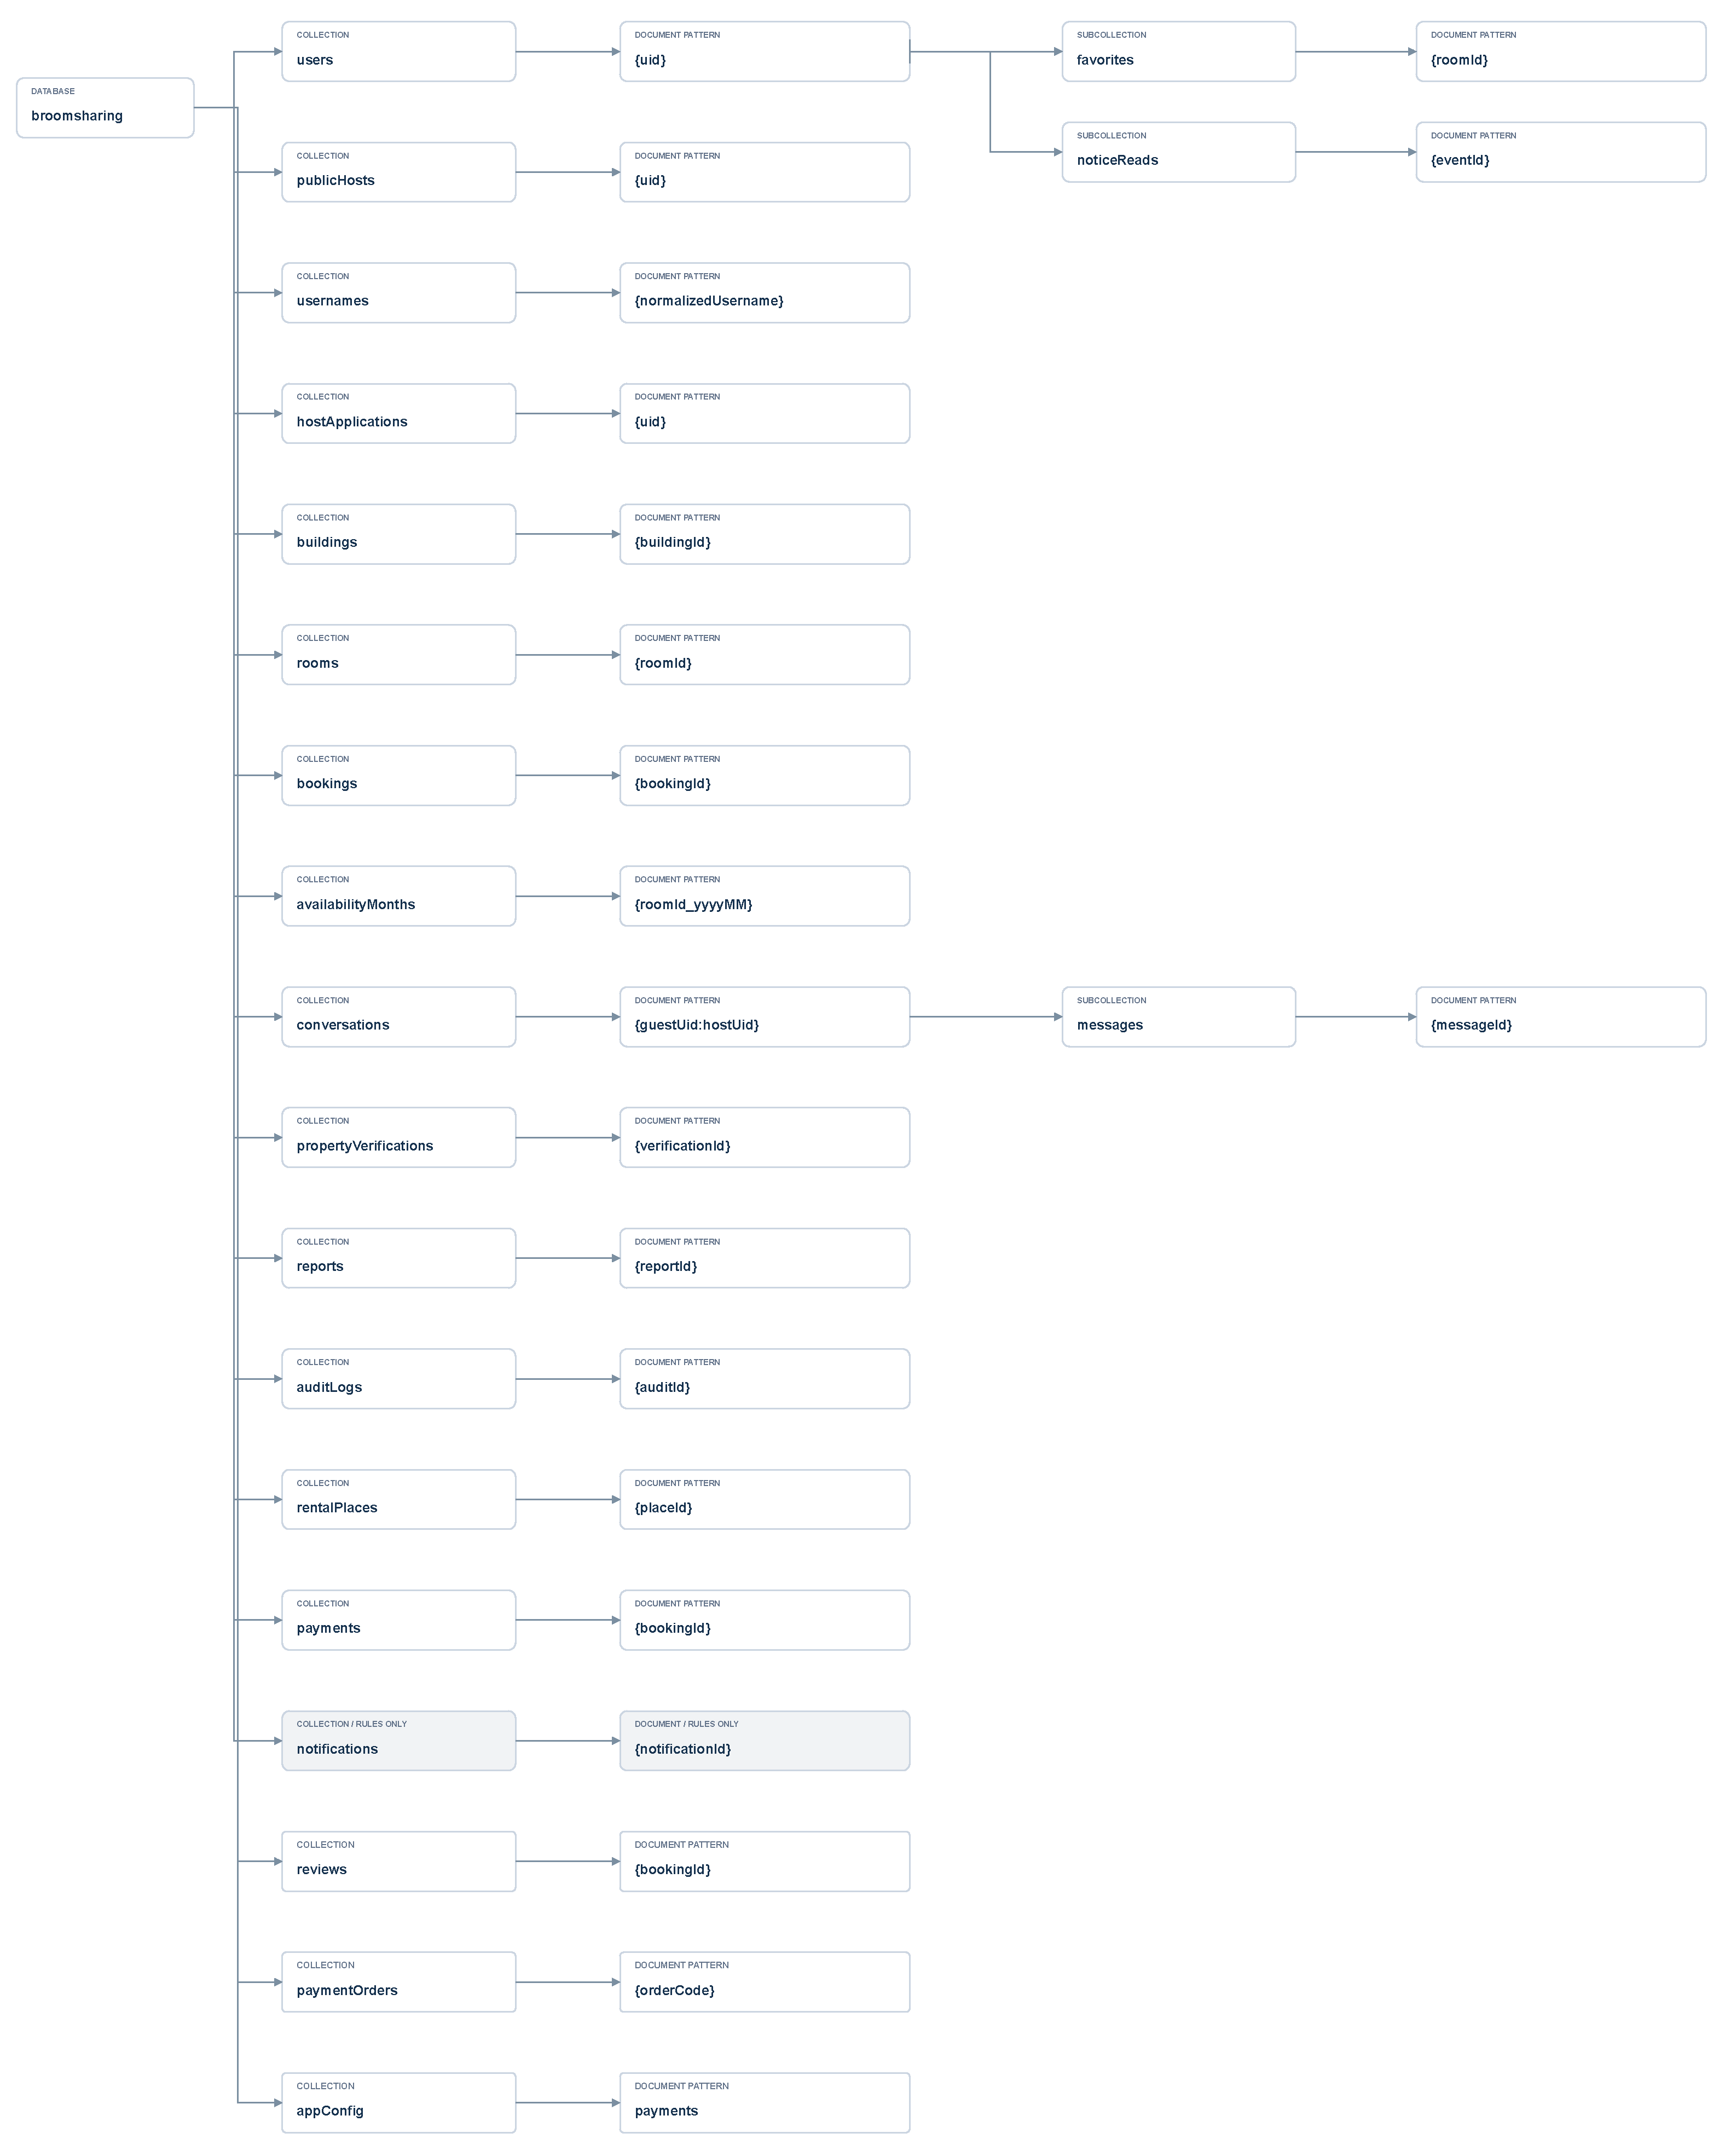
\includegraphics[width=\textwidth,height=0.86\textheight,keepaspectratio]{chapter4/firestore-overview.pdf}
\caption{Cây lưu trữ Firestore BroomSharing. Thẻ màu xám là contract thông báo cũ trong Rules.}
\label{fig:ch4-overview}
\end{figure}
\clearpage
\begin{landscape}
\pagestyle{empty}
\BroomLandscapePagetrue
\begin{figure}[p]
\centering
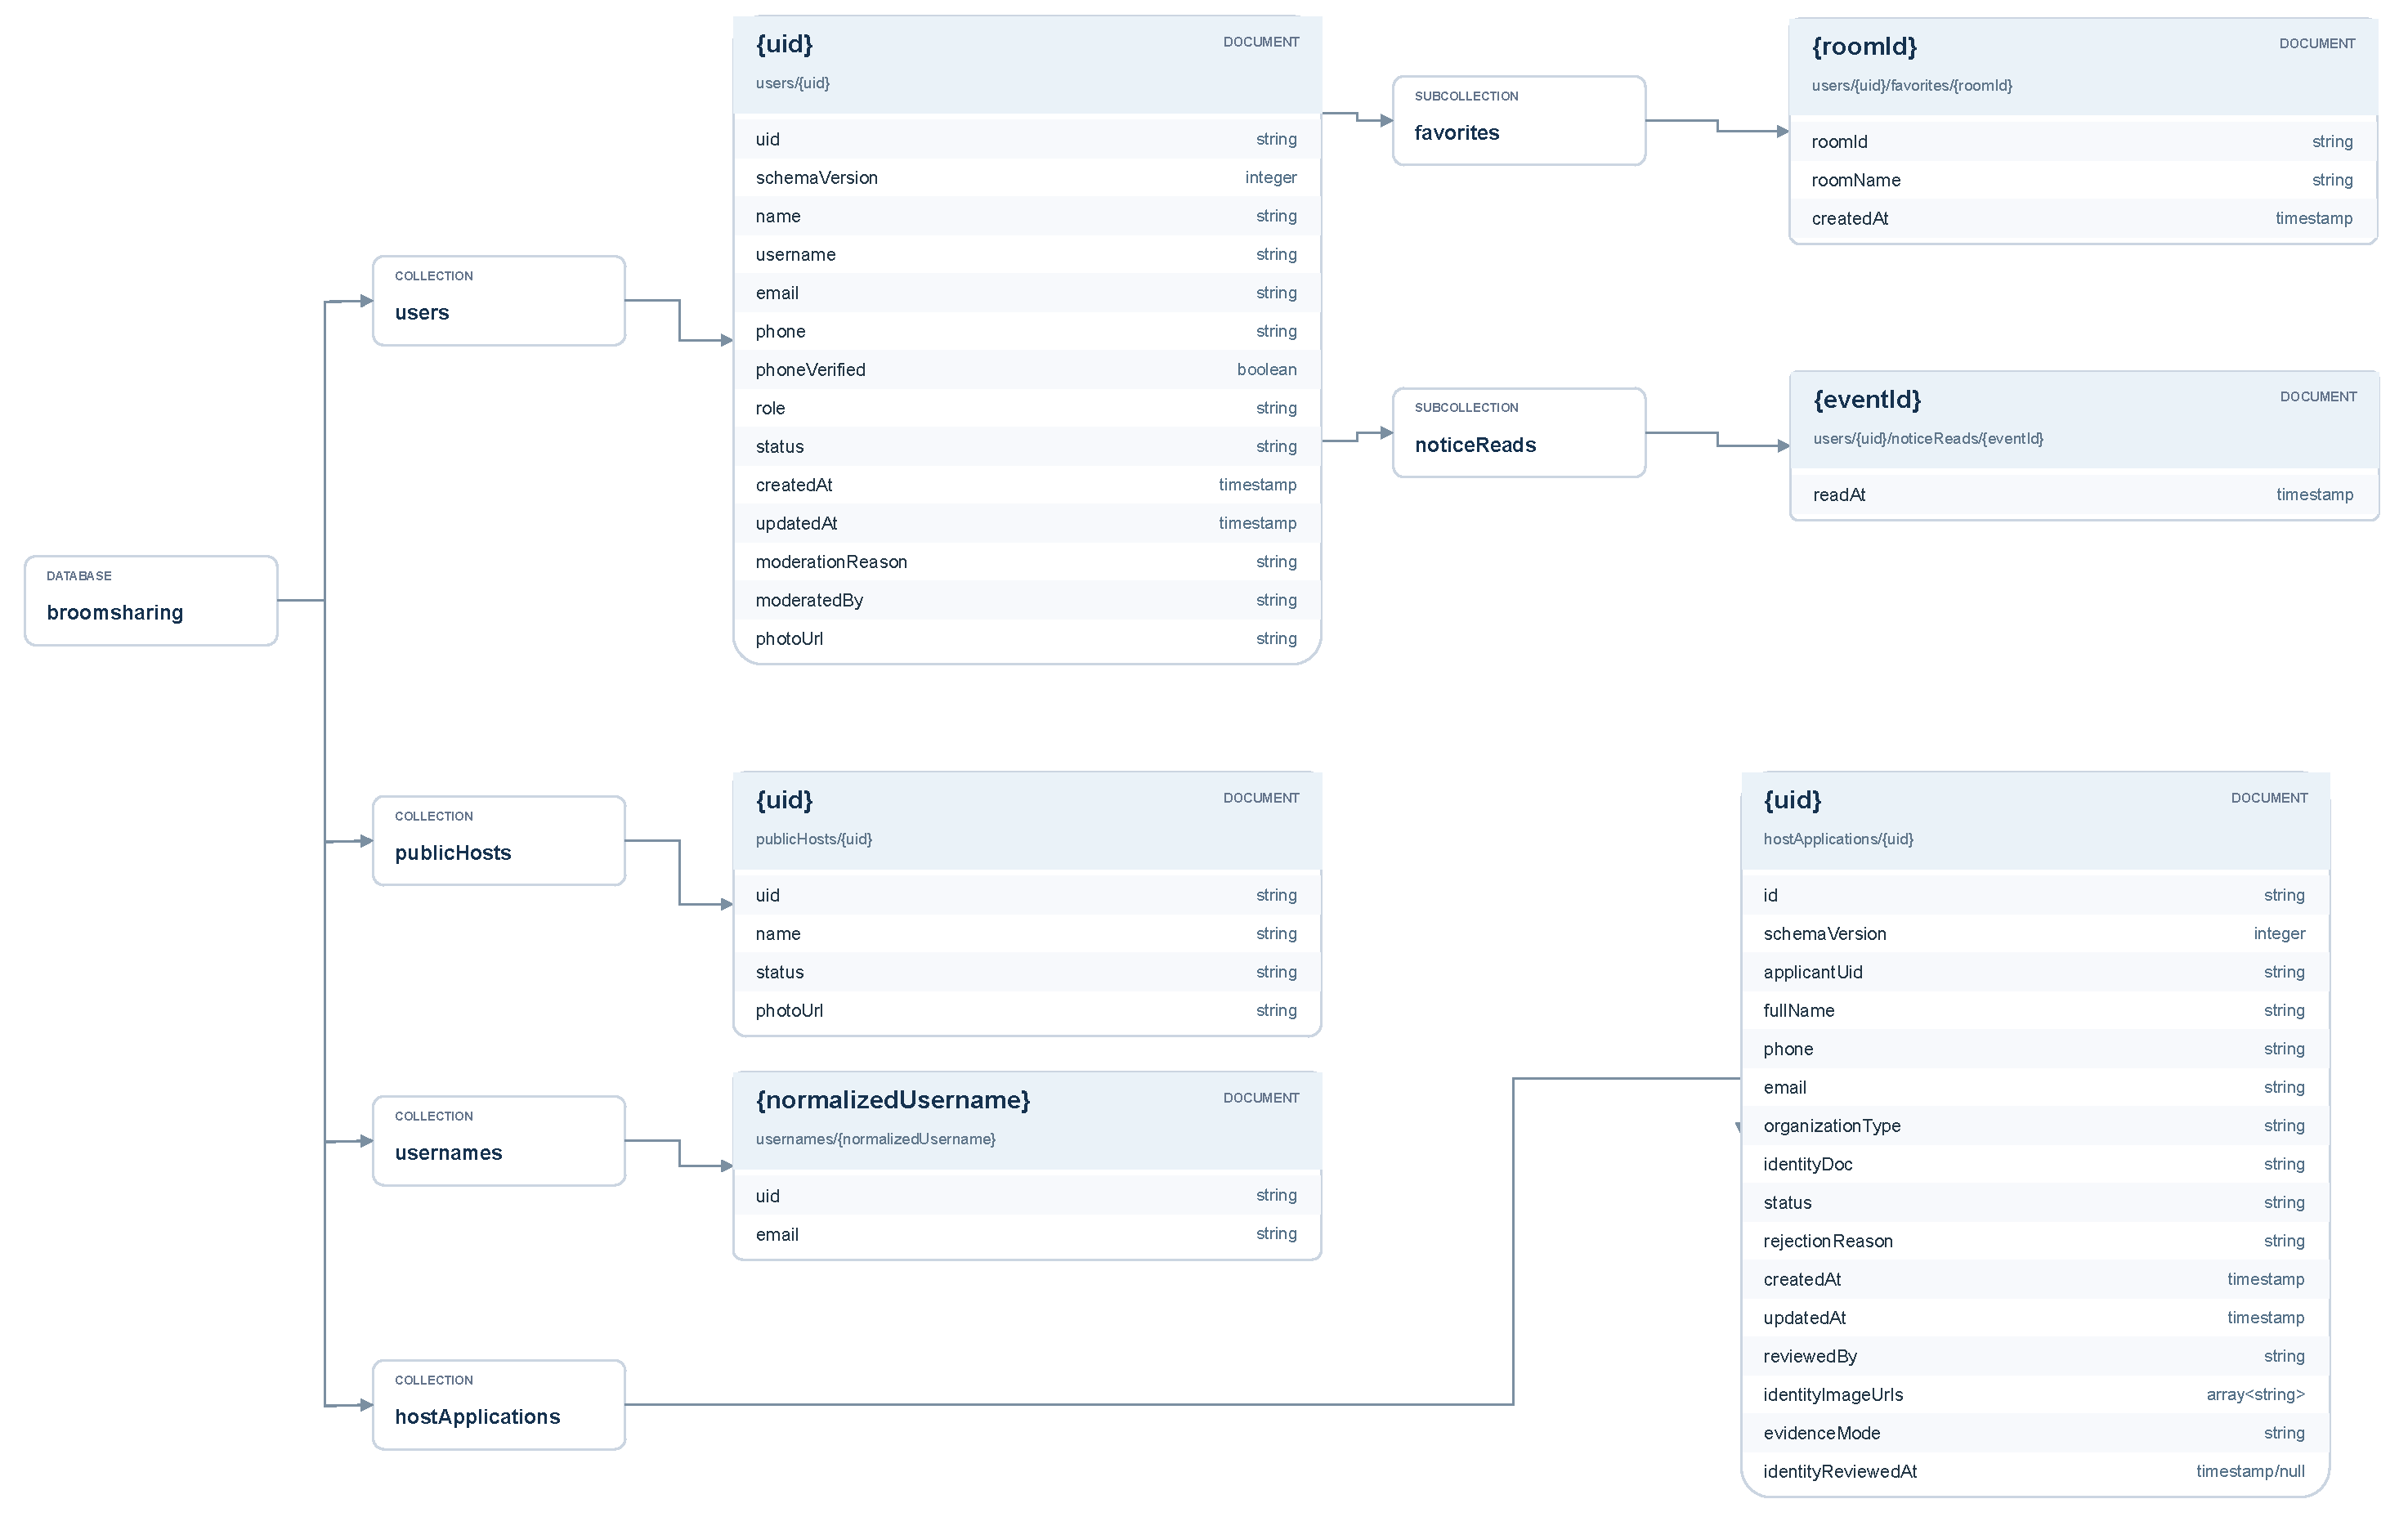
\includegraphics[width=\linewidth,height=0.82\textheight,keepaspectratio]{chapter4/firestore-accounts.pdf}
\caption{Cấu trúc nhóm tài khoản và các subcollection thuộc hồ sơ người dùng.}
\label{fig:ch4-accounts}
\end{figure}
\clearpage
\begin{figure}[p]
\centering
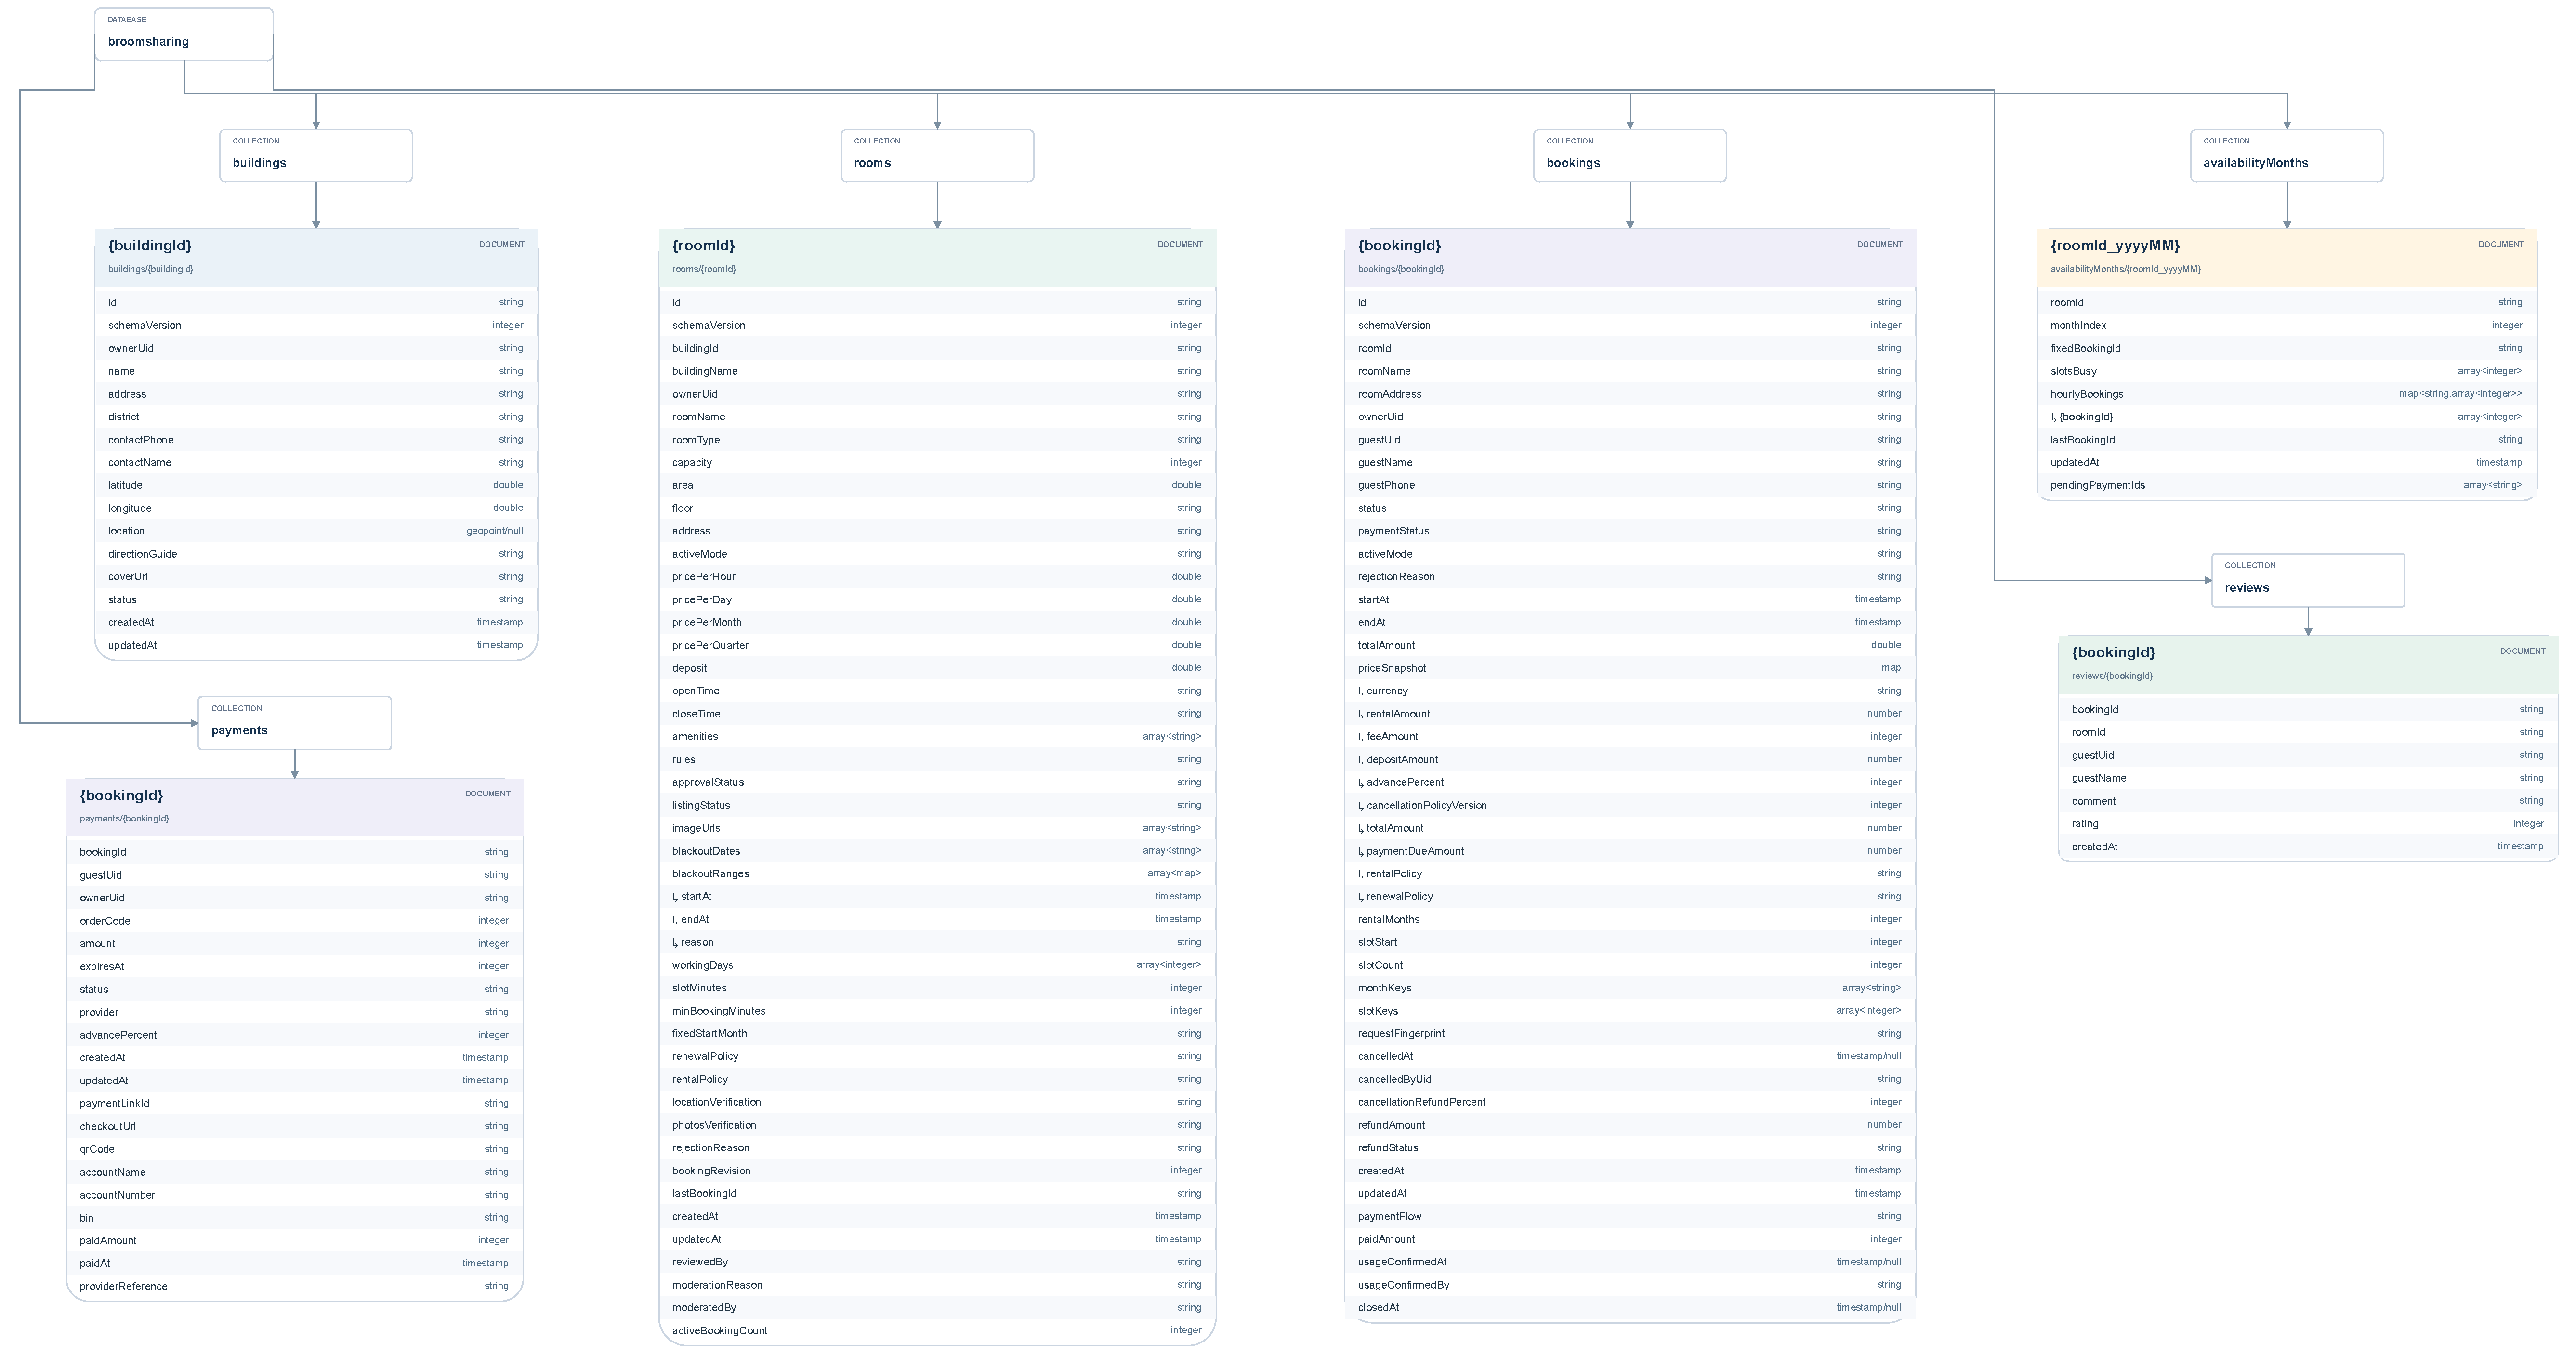
\includegraphics[width=\linewidth,height=0.82\textheight,keepaspectratio]{chapter4/firestore-booking.pdf}
\caption{Cấu trúc tài sản, booking, lịch tháng, thanh toán và đánh giá. Các collection nằm ngang cấp trong database.}
\label{fig:ch4-booking}
\end{figure}
\clearpage
\begin{figure}[p]
\centering
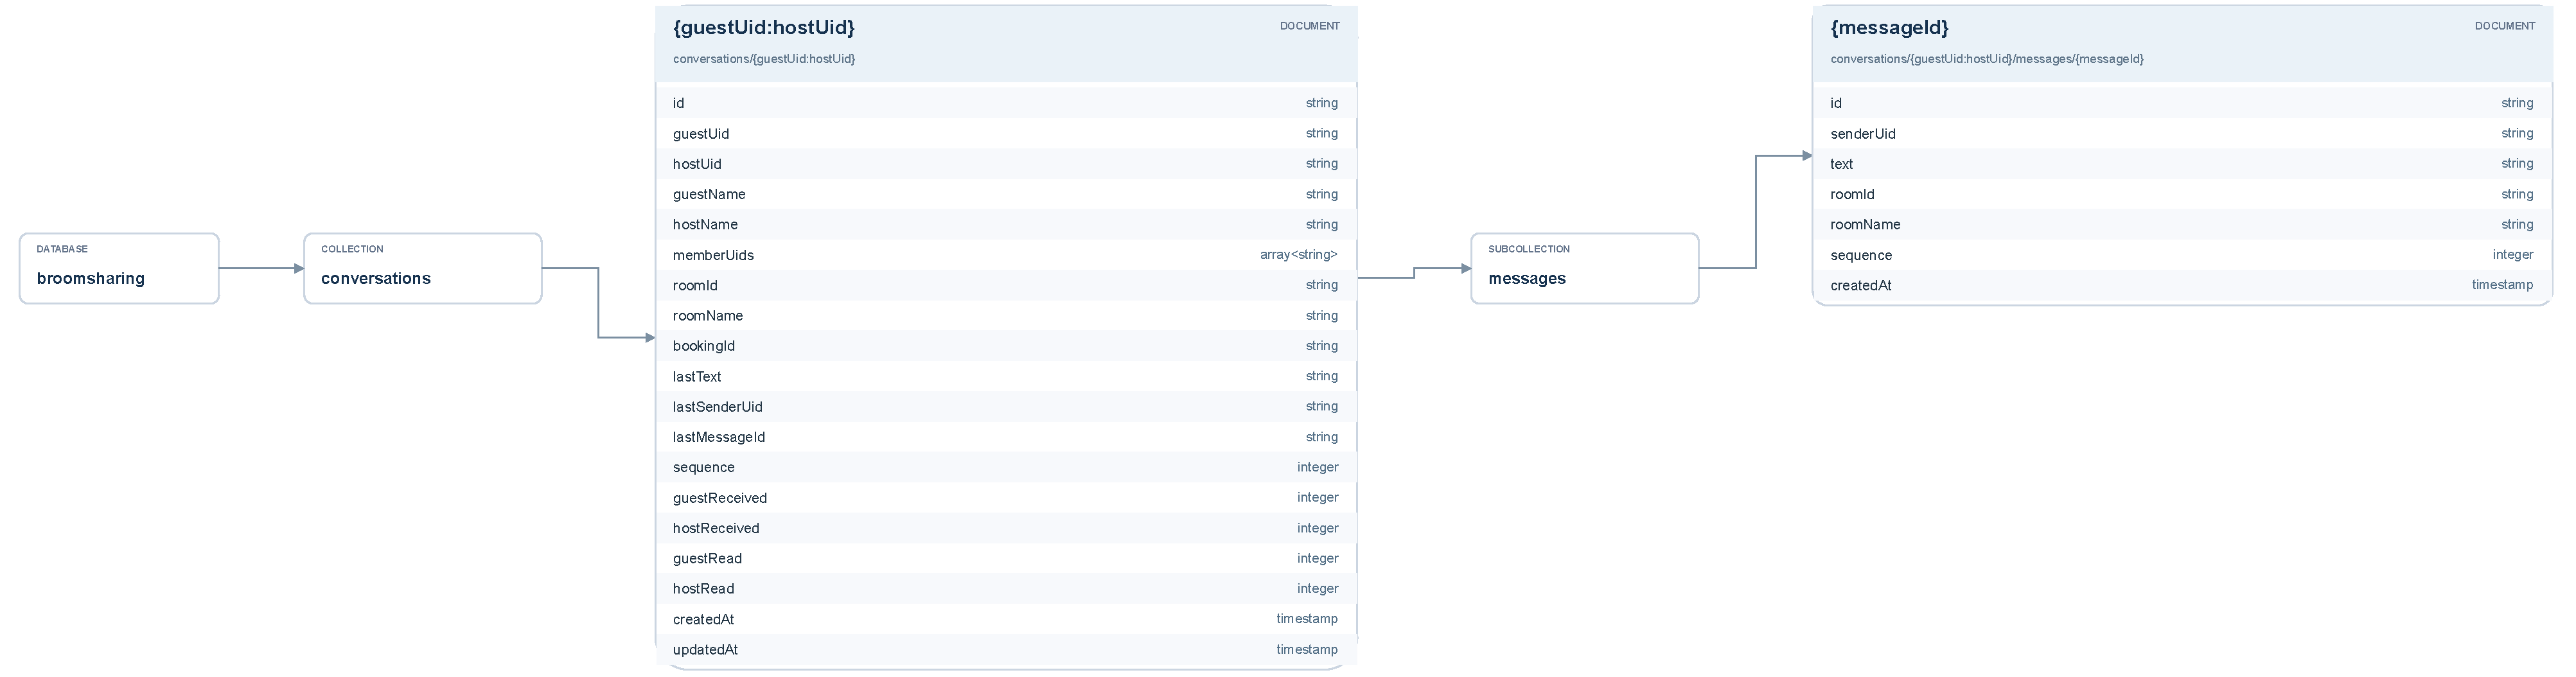
\includegraphics[width=\linewidth,height=0.82\textheight,keepaspectratio]{chapter4/firestore-chat.pdf}
\caption{Cấu trúc hội thoại và subcollection tin nhắn của từng hội thoại.}
\label{fig:ch4-chat}
\end{figure}
\clearpage
\begin{figure}[p]
\centering
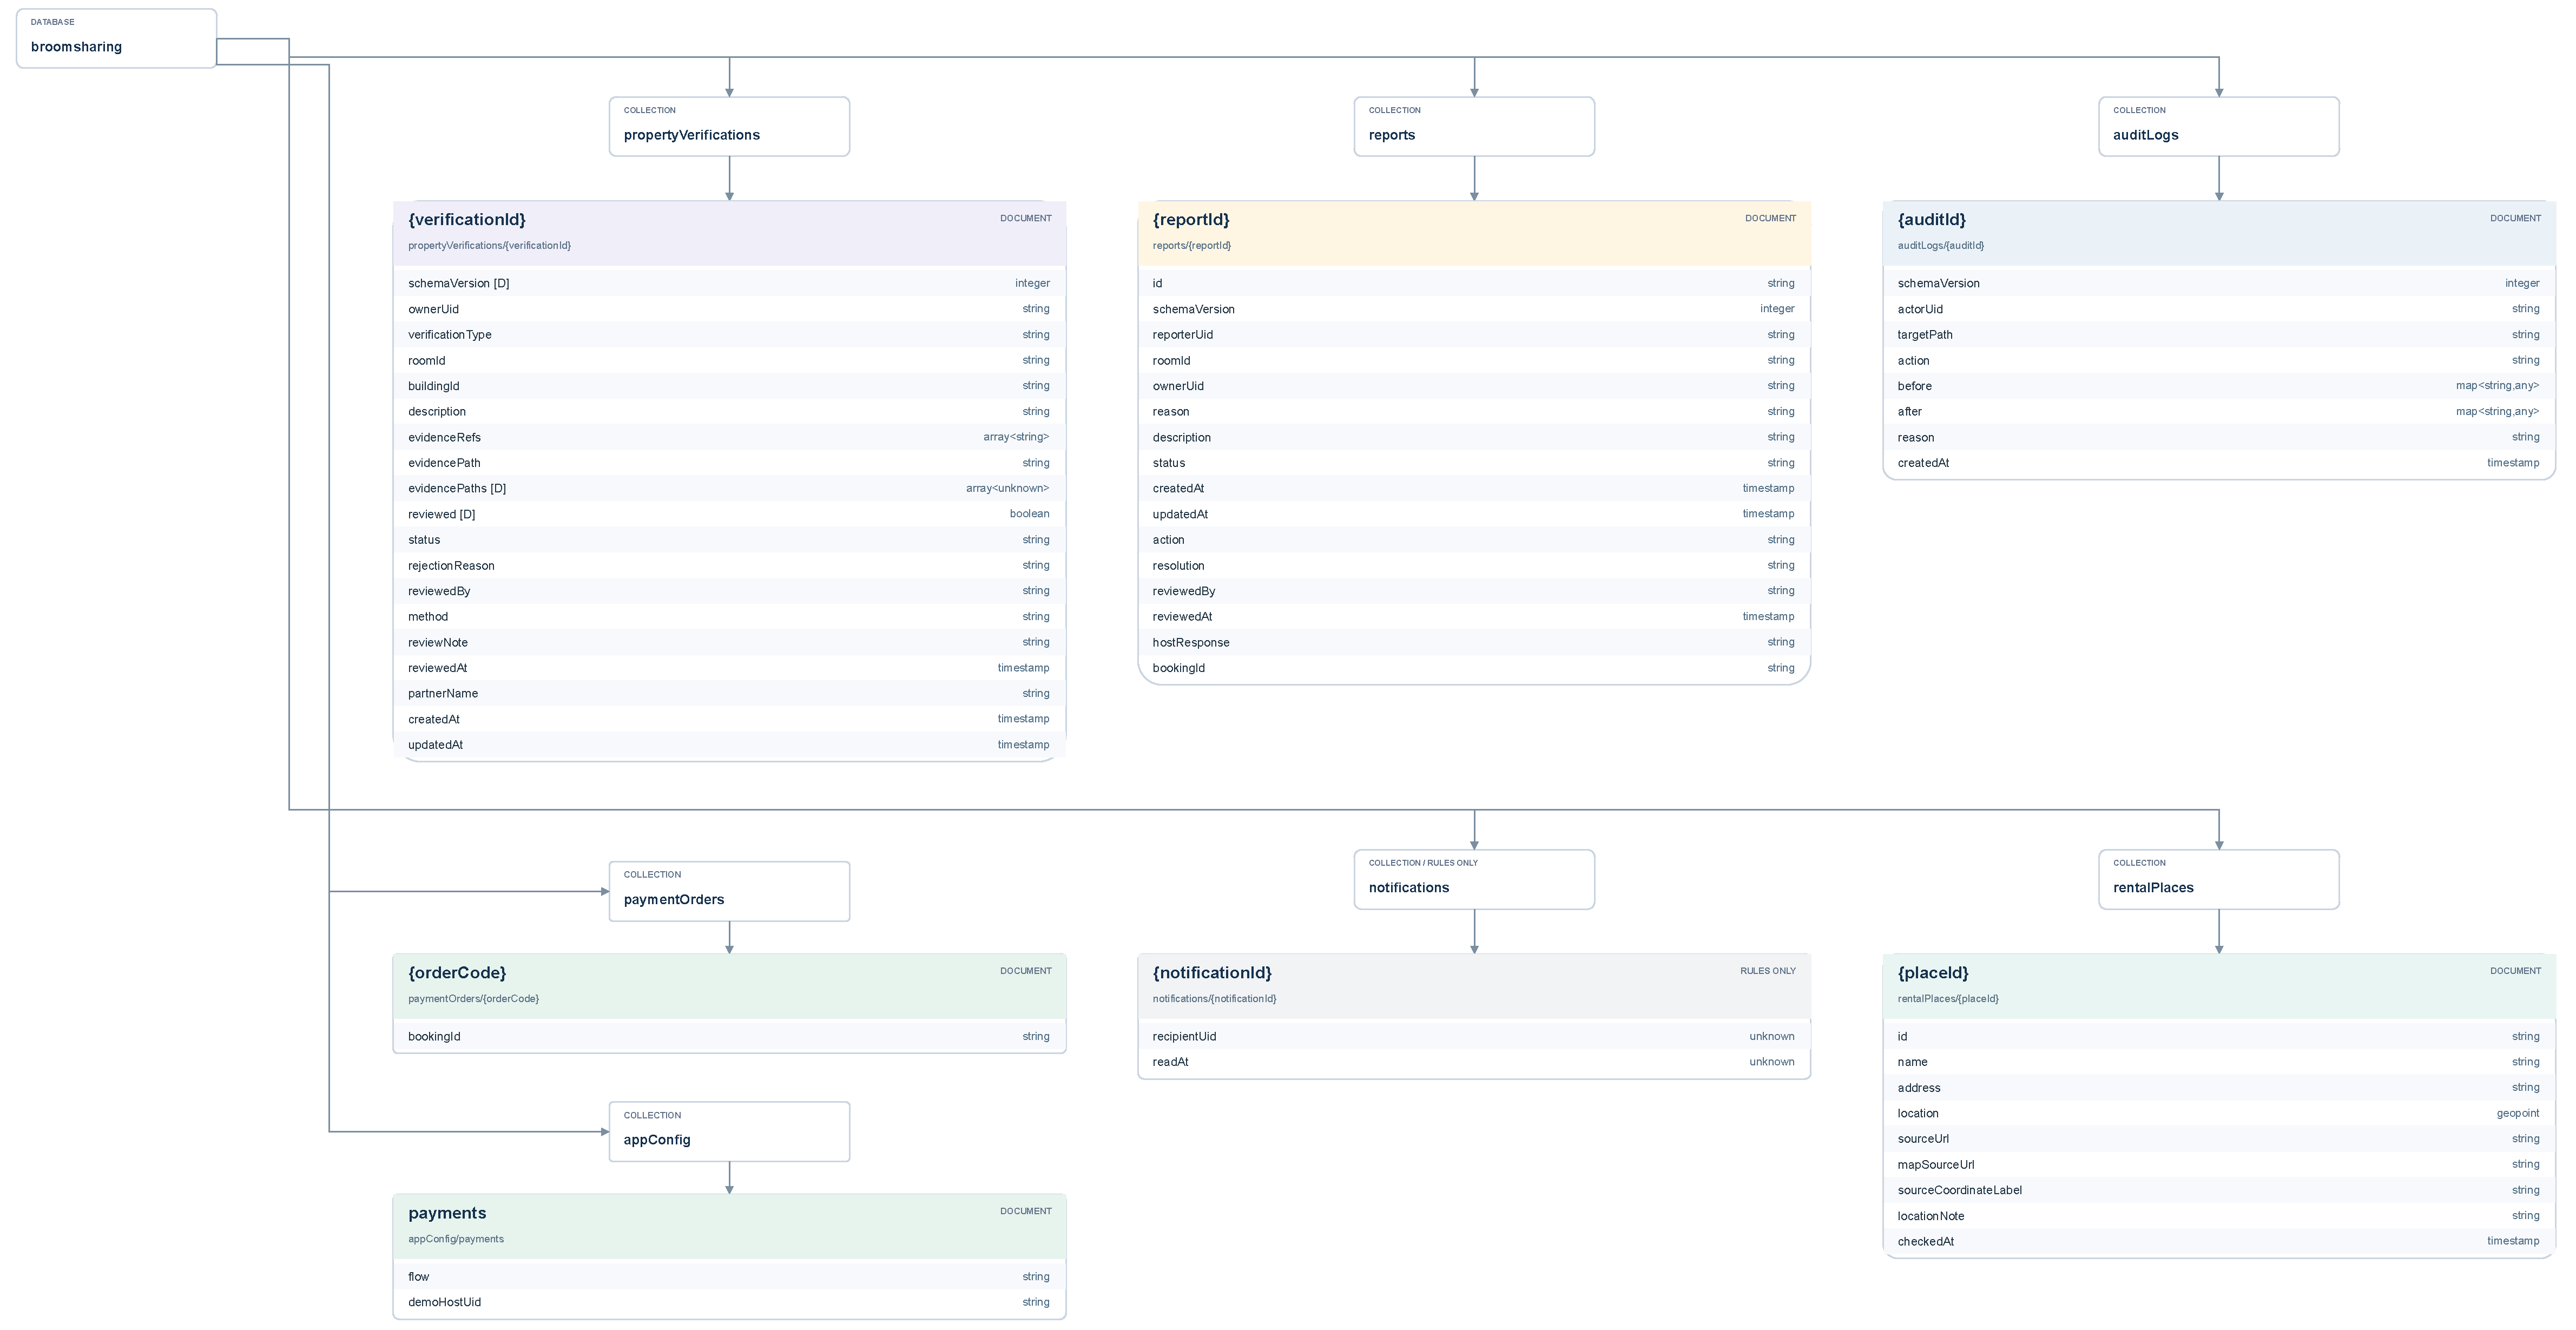
\includegraphics[width=\linewidth,height=0.82\textheight,keepaspectratio]{chapter4/firestore-administration.pdf}
\caption{Nhóm quản trị, dữ liệu tham khảo và cấu hình backend. [D] là trường từ dữ liệu mẫu; Rules-only là contract chưa có luồng ghi hiện tại.}
\label{fig:ch4-administration}
\end{figure}
\clearpage
\BroomLandscapePagefalse
\end{landscape}


Nhóm tài khoản trong Hình~\ref{fig:ch4-accounts} dùng chung UID để liên kết hồ sơ, bản chiếu Host và đơn đăng ký. Nhóm đặt chỗ trong Hình~\ref{fig:ch4-booking} liên kết tài sản với booking và lịch tháng bằng ID. Trong nhóm chat, mỗi document hội thoại sở hữu một subcollection tin nhắn riêng (Hình~\ref{fig:ch4-chat}); dữ liệu xác minh, báo cáo và nhật ký lưu thêm ID hoặc đường dẫn của đối tượng được xử lý (Hình~\ref{fig:ch4-administration}). Các liên kết logic này có ý nghĩa và bội số như Bảng~\ref{tab:ch4-relations-summary}.

\begingroup\small\setstretch{1.08}
\begin{longtable}{@{}>{\raggedright\arraybackslash}p{4.2cm}>{\raggedright\arraybackslash}p{5.15cm}>{\raggedright\arraybackslash}p{5.9cm}@{}}
\caption{Các quan hệ logic chính}\label{tab:ch4-relations-summary}\\
\toprule Nhóm dữ liệu & Liên kết & Ý nghĩa và bội số \\ \midrule\endfirsthead
\toprule Nhóm dữ liệu & Liên kết & Ý nghĩa và bội số \\ \midrule\endhead
\bottomrule\endlastfoot
Tài khoản & UID của hồ sơ, alias và bản chiếu Host. & Một User có một alias theo luồng đăng ký và tối đa một bản chiếu Host; UID liên kết với Authentication. \\
Tài sản & \texttt{rooms.\allowbreak{}building\allowbreak{}Id}; owner UID của Room và Building. & Một Building có nhiều Room; mỗi Room gắn với một Building và Host sở hữu tương ứng. \\
Đặt chỗ & Room ID, guest UID, owner UID. & Mỗi Booking thuộc một Room và hai bên tham gia; một Room có nhiều booking qua thời gian. \\
Lịch tháng & Room ID; fixed booking ID; khóa booking trong \texttt{hourly\allowbreak{}Bookings}. & Mỗi Room có nhiều tháng lịch; một tháng giữ toàn bộ cho một booking cố định hoặc giữ các slot thuê giờ. \\
Yêu thích & Room ID trong nhánh của User. & Quan hệ nhiều với nhiều giữa User và Room thông qua Favorite. \\
Hội thoại & \texttt{member\allowbreak{}Uids}; Room ID, Booking ID; sender UID của message. & Hai thành viên trong một hội thoại; một hội thoại có nhiều message và ngữ cảnh phòng hoặc booking. \\
Quản trị & UID chủ hồ sơ, người báo cáo, người duyệt; Room ID hoặc Building ID. & Hồ sơ xác minh và báo cáo liên kết tới đối tượng được xử lý; liên kết phụ thuộc loại hồ sơ. \\
Thanh toán & Booking ID của Payment; booking ID trong PaymentOrder. & Mỗi booking dùng một Payment cùng ID; order code ánh xạ về booking để đối soát webhook. Payment không phải subcollection của Booking.  \\
Nhật ký & Actor UID và \texttt{target\allowbreak{}Path}. & Actor xác định tài khoản hoặc tiến trình backend; đường dẫn đích thay đổi theo hành động. \\
\end{longtable}\endgroup

Map \texttt{price\allowbreak{}Snapshot} giữ giá và chính sách của booking; mảng \texttt{blackout\allowbreak{}Ranges} chứa các khoảng khóa lịch; map \texttt{hourly\allowbreak{}Bookings} ánh xạ booking ID tới tập slot. Đây là dữ liệu nhúng trong document. Room được thuê độc quyền trong khoảng $[startAt,endAt)$: PENDING giữ lịch tạm chờ thanh toán trong tối đa 5 phút, HOURLY dùng slot 30 phút và FIXED giữ trọn một hoặc ba tháng. Mảng \texttt{pending\allowbreak{}Payment\allowbreak{}Ids} phân biệt các khóa tạm chờ thanh toán với lịch đã xác nhận. Transaction duy trì sự nhất quán giữa booking, lịch tháng và revision của phòng.

\subsection{Một số thao tác dữ liệu tiêu biểu}
\label{sec:ch4-operations}

\subsubsection{Các nhóm thao tác dữ liệu}

Các Repository thực hiện ba nhóm thao tác: đọc dữ liệu theo điều kiện, theo dõi thay đổi bằng listener và ghi dữ liệu nghiệp vụ. Truy vấn danh sách giới hạn phạm vi theo trạng thái hoặc UID; listener cập nhật booking và trao đổi giữa hai bên; transaction xử lý những thay đổi liên quan nhiều document. Bảng~\ref{tab:ch4-operations} tổng hợp các thao tác tiêu biểu và dữ liệu tham gia.

\begingroup\small\setstretch{1.08}
\begin{longtable}{@{}>{\raggedright\arraybackslash}p{3.45cm}>{\raggedright\arraybackslash}p{4.25cm}>{\raggedright\arraybackslash}p{7.55cm}@{}}
\caption{Các thao tác dữ liệu tiêu biểu trong ứng dụng}\label{tab:ch4-operations}\\
\toprule Thao tác & Dữ liệu & Cách xử lý trong Repository \\ \midrule\endfirsthead
\toprule Thao tác & Dữ liệu & Cách xử lý trong Repository \\ \midrule\endhead
\midrule\multicolumn{3}{r}{\small Còn tiếp ở trang sau}\\\endfoot
\bottomrule\endlastfoot
Tải danh sách phòng & \texttt{rooms}; bổ sung Building và PublicHost. & Lọc APPROVED, ACTIVE; sắp theo document ID, lấy tối đa 20 phòng và phân trang bằng con trỏ. \\
Theo dõi booking & \texttt{bookings}. & Lọc \texttt{guest\allowbreak{}Uid} hoặc \texttt{owner\allowbreak{}Uid} theo tài khoản; nhận thay đổi qua listener. \\
Đọc lịch phòng & \texttt{availability\allowbreak{}Months}. & Đọc các document tháng liên quan để xác định lịch giữ chỗ theo giờ hoặc theo tháng. \\
Tạo booking & Booking, lịch tháng, Room và AuditLog. & Đọc và kiểm tra trong transaction; ghi booking PENDING cùng khóa lịch, revision phòng và nhật ký. \\
Chuyển trạng thái booking & Booking, lịch tháng, Room và AuditLog. & Kiểm tra bên thực hiện, trạng thái và thời gian; hủy, hết hạn hoặc khép lượt giải phóng khóa lịch tương ứng; booking mới được backend xác nhận sau thanh toán. \\
Đối soát thanh toán & Payment, Booking, lịch tháng, Room và AuditLog. & Backend kiểm tra kết quả payOS; xác nhận khi nhận đủ tiền đúng hạn hoặc khép link chưa trả và nhả lịch, không tự hoàn tiền.  \\
Theo dõi chat & \texttt{conversations} và subcollection \texttt{messages}. & Inbox lọc UID trong \texttt{member\allowbreak{}Uids}; tin nhắn sắp theo \texttt{sequence}, giới hạn số lượng và nhận cập nhật qua listener. \\
Gửi tin nhắn & Message và document hội thoại cha. & Transaction ghi tin, cập nhật preview, thứ tự và bộ đếm nhận tin của bên còn lại. \\
Lưu phòng yêu thích & \texttt{users/\allowbreak{}\{uid\}/\allowbreak{}favorites/\allowbreak{}\{room\allowbreak{}Id\}}. & Ghi ID, tên phòng và thời điểm lưu; bỏ yêu thích bằng cách xóa document tại cùng đường dẫn. \\
\end{longtable}\endgroup

Thao tác đọc danh sách và theo dõi thay đổi phục vụ hai nhu cầu khác nhau. Danh sách phòng được tải theo từng trang, còn booking và chat cần phản ánh cập nhật trong quá trình sử dụng. Các listener này bỏ qua snapshot từ cache hoặc còn ghi đang chờ xác nhận, thông qua metadata \texttt{isFrom\allowbreak{}Cache()} và \texttt{hasPending\allowbreak{}Writes()} \parencite{firebase_listeners}.

\Needspace{15\baselineskip}
\subsubsection{Các truy vấn tiêu biểu}

Khi tải danh sách không gian, \texttt{Room\allowbreak{}Repository.\allowbreak{}page()} chỉ chọn phòng đã duyệt APPROVED và đang hiển thị ACTIVE. Tham số \texttt{after} là document ID cuối của lượt tải trước; ở lượt đầu, tham số này bằng \texttt{null}. Truy vấn sắp xếp theo document ID và giới hạn bằng hằng \texttt{PAGE\_SIZE=20}; \texttt{start\allowbreak{}After()} đặt điểm bắt đầu cho lượt tiếp theo \parencite{firebase_queries,firebase_query_cursors}.

\par\medskip\noindent\begin{minipage}{\linewidth}
\inputminted[firstnumber=1]{java}{Resources/chapter4/code/room-query.java}
{\footnotesize\noindent Nguồn: \texttt{Room\allowbreak{}Repository.\allowbreak{}java}, dòng 63 đến 70.\par}
\end{minipage}\par\medskip

Kết quả được đọc từ máy chủ bằng \texttt{get(Source.\allowbreak{}SERVER)}. Repository lấy ID của document cuối làm con trỏ, rồi đọc bổ sung Building và PublicHost để tạo danh sách \texttt{Room\allowbreak{}Listing}. Khi không có document, con trỏ giữ giá trị trước đó. Cờ \texttt{hasMore} được đặt theo điều kiện số document bằng 20; đây là căn cứ cho phép thử tải tiếp, chưa khẳng định lượt kế tiếp chắc chắn còn dữ liệu. Lỗi truy vấn được chuyển tới callback lỗi, tách khỏi trường hợp truy vấn thành công nhưng danh sách rỗng.

\texttt{Room\allowbreak{}ViewModel} gọi \texttt{page()}, cập nhật con trỏ và ghép kết quả theo Room ID để tránh trùng phòng. Khi có từ khóa hoặc bộ lọc, ViewModel tự tải các trang còn lại trước khi kết luận không có kết quả; danh sách được phát qua \texttt{LiveData}; \texttt{Main\allowbreak{}Activity} quan sát kết quả để cập nhật danh sách và nút tải thêm.

Với danh sách booking, \texttt{Booking\allowbreak{}Repository.\allowbreak{}watchMine()} lọc \texttt{guest\allowbreak{}Uid} bằng UID hiện tại qua hàm dùng chung \texttt{watch\allowbreak{}Participant()}. Listener nhận thay đổi từ Firestore và chỉ chuyển snapshot đã được máy chủ xác nhận tới callback. Các document được ánh xạ thành \texttt{Booking}, sắp theo thời điểm tạo booking giảm dần rồi trả về ViewModel.

\par\medskip\noindent\begin{minipage}{\linewidth}
\inputminted[firstnumber=1]{java}{Resources/chapter4/code/booking-query-listener.java}
{\footnotesize\noindent Nguồn: \texttt{Booking\allowbreak{}Repository.\allowbreak{}java}, dòng 659 đến 671.\par}
\end{minipage}\par\medskip

\texttt{Booking\allowbreak{}ViewModel.\allowbreak{}watchMine()} đặt trạng thái tải, gọi Repository và cập nhật \texttt{bookings} bằng \texttt{UiState.\allowbreak{}success()} hoặc \texttt{UiState.\allowbreak{}error()}. \texttt{My\allowbreak{}Bookings\allowbreak{}Activity} quan sát \texttt{LiveData} này để hiển thị dữ liệu và lọc trạng thái tại giao diện. Khi màn hình dừng, listener được gỡ; khi hiển thị lại, truy vấn được đăng ký lại để nhận các thay đổi tiếp theo.

\subsubsection{Tạo booking bằng transaction}

Khi người thuê gửi yêu cầu, \texttt{Booking\allowbreak{}Repository.\allowbreak{}create()} phải xác nhận phòng còn nhận đặt và khoảng thuê chưa bị chiếm. Booking ID được băm từ UID cùng \texttt{request\allowbreak{}Key}; trường \texttt{request\allowbreak{}Fingerprint} biểu diễn nội dung yêu cầu. Nếu document theo ID này đã tồn tại và fingerprint trùng khớp, phương thức trả lại booking ID cũ. Nếu fingerprint khác, yêu cầu bị từ chối, tránh dùng lại cùng mã gửi cho một lựa chọn khác.

Trong callback \texttt{run\allowbreak{}Transaction()}, Repository đọc hồ sơ người thuê, phòng, bản chiếu Host, tòa nhà, cấu hình \texttt{appConfig/payments} và các tháng lịch liên quan. Booking mới phải thuộc Host của kênh demo với luồng \texttt{INSTANT\_5M}. Tài khoản phải ACTIVE và có vai trò GUEST hoặc HOST; phòng phải APPROVED, ACTIVE và không thuộc chính người thuê. Host cùng tòa nhà phải còn hoạt động, đồng thời owner UID của Room phải khớp Building. Giá và thời gian thuê được tính lại từ dữ liệu phòng bằng \texttt{Booking\allowbreak{}Policy.\allowbreak{}plan()}, sau đó lịch được kiểm tra trước mọi lệnh ghi.

\par\medskip\noindent\begin{minipage}{\linewidth}
\inputminted[firstnumber=1]{java}{Resources/chapter4/code/booking-prepare.java}
{\footnotesize\noindent Nguồn: \texttt{Booking\allowbreak{}Repository.\allowbreak{}java}, dòng 206 đến 217.\par}
\end{minipage}\par\medskip

Hàm \texttt{months()} đọc lịch tháng bằng chính transaction. Với thuê giờ, \texttt{reserve()} kiểm tra tập slot mới không giao với \texttt{slotsBusy}; với thuê cố định, tháng phải chưa có booking cố định hoặc booking giờ. Nếu có xung đột, hàm phát sinh lỗi trước bước ghi. Khi hợp lệ, các đối tượng lịch được cập nhật trong bộ nhớ rồi ghi cùng booking, revision của phòng và nhật ký.

\par\medskip\noindent\begin{minipage}{\linewidth}
\inputminted[firstnumber=1]{java}{Resources/chapter4/code/booking-commit.java}
{\footnotesize\noindent Nguồn: \texttt{Booking\allowbreak{}Repository.\allowbreak{}java}, dòng 226 đến 237.\par}
\end{minipage}\par\medskip

Firestore áp dụng toàn bộ các lệnh ghi trong transaction theo tính nguyên tử và có thể chạy lại callback khi document đã đọc bị thay đổi đồng thời \parencite{firebase_transaction}. Vì các yêu cầu cùng phòng đọc và cập nhật lịch tháng chung, việc kiểm tra xung đột được thực hiện lại trên lịch mới khi transaction chạy lại. Callback thành công trả về booking ID sau khi giao dịch hoàn tất; lỗi kiểm tra, xung đột hoặc lỗi ghi được chuyển tới callback lỗi. Kết quả ghi thành công là booking PENDING và phần lịch tạm giữ; đây chưa phải xác nhận đã thanh toán. Màn hình QR được mở ngay để tiếp tục cùng booking.

Booking mới lưu \texttt{schema\allowbreak{}Version=\allowbreak{}2}, giá và chính sách tại thời điểm đặt trong \texttt{price\allowbreak{}Snapshot}. Trường \texttt{paymentFlow=INSTANT\_5M} xác định luồng giữ lịch tạm. Trước khi tạo yêu cầu payOS, booking chưa ghi nhận tiền; sau đó Payment theo dõi mã đơn, số tiền, QR và thời hạn. Backend đối chiếu kết quả nhà cung cấp, số tiền và thời điểm nhận tiền trước khi xác nhận \texttt{PAID/CONFIRMED}. Khi link đã kết thúc mà chưa trả tiền, backend chuyển booking sang \texttt{EXPIRED}, nhả đúng khóa lịch và giữ lịch sử. Tiền đến muộn, sai số tiền hoặc lịch không còn hợp lệ được đưa vào \texttt{REVIEW\_REQUIRED}; chưa có API hoàn tiền tự động.

\Needspace{8\baselineskip}
\subsection{Phân quyền và bảo vệ dữ liệu}
\label{sec:ch4-security}

Firestore Rules kết hợp UID, vai trò, trạng thái ACTIVE và quyền sở hữu để kiểm soát truy cập. Guest và Host đều có quyền thuê, nhưng không được tự đặt phòng của mình. Bảng~\ref{tab:ch4-permissions} tóm tắt các nhóm quyền chính; các thao tác ngoài nhánh được cho phép chịu quy tắc từ chối mặc định.

\begingroup\small\setstretch{1.08}
\begin{longtable}{@{}>{\raggedright\arraybackslash}p{4.1cm}>{\raggedright\arraybackslash}p{11.15cm}@{}}
\caption{Phân quyền theo nhóm dữ liệu}\label{tab:ch4-permissions}\\
\toprule Nhóm & Quyền truy cập chính \\ \midrule\endfirsthead
\toprule Nhóm & Quyền truy cập chính \\ \midrule\endhead
\bottomrule\endlastfoot
Hồ sơ và đơn Host & Chủ hồ sơ hoặc Admin được đọc. Người dùng sửa nhóm trường hồ sơ cho phép; Guest nộp đơn, Admin xét duyệt. PublicHost được đọc bởi tài khoản hoạt động. \\
Alias và dữ liệu cá nhân & \texttt{usernames} cho phép get trước đăng nhập, list chỉ dành cho Admin. Favorite và mốc đã đọc thuộc quyền tài khoản sở hữu nhánh dữ liệu. \\
Tòa nhà và phòng & Host quản lý tài sản của mình; Admin được cập nhật Room, không có nhánh ghi Building riêng. Phòng công khai cho tài khoản hoạt động khi APPROVED và ACTIVE. \\
Booking và lịch & Hai bên tham gia và Admin được đọc Booking. Chuyển trạng thái phụ thuộc vai trò, thời gian và lịch; Admin không có nhánh chuyển tùy ý. Ghi lịch phải khớp booking trong cùng thao tác. \\
Thanh toán và cấu hình & Người thuê, Host liên quan và Admin được đọc Payment; client không được tự ghi trạng thái tiền. PaymentOrder chỉ do backend truy cập; cấu hình kênh cho tài khoản hoạt động đọc, không chứa khóa payOS.  \\
Chat & Chỉ thành viên đang hoạt động đọc hội thoại và message. Gửi tin cập nhật đồng thời preview, thứ tự và bộ đếm; mỗi bên chỉ tăng mốc đã đọc của mình. Admin không có quyền đọc riêng. \\
Quản trị và tham khảo & Chủ hồ sơ hoặc Admin đọc xác minh; Admin cập nhật kết quả. Báo cáo được đọc theo người gửi, Host liên quan hoặc Admin. Audit chỉ Admin đọc; RentalPlace chỉ cho tài khoản hoạt động đọc. \\
\end{longtable}\endgroup

Quyền ghi còn phụ thuộc nội dung và tính nhất quán giữa document. Rules dùng danh sách trường cho phép và \texttt{diff().\allowbreak{}affected\allowbreak{}Keys()} để giới hạn thay đổi; \texttt{get\allowbreak{}After()} kiểm tra trạng thái sau ghi của các document liên quan \parencite{firebase_rules_fields,firebase_rules_conditions}. Ví dụ, \texttt{held\allowbreak{}Month()} đối chiếu booking với lịch tháng trước khi chấp nhận thao tác giữ chỗ.

\par\medskip\noindent\begin{minipage}{\linewidth}
\inputminted[firstnumber=1]{text}{Resources/chapter4/code/rules-held-month.txt}
{\footnotesize\noindent Nguồn: \texttt{firestore.\allowbreak{}rules}, dòng 24 đến 30.\par}
\end{minipage}\par\medskip

Backend dùng Firebase Admin SDK nên phải tự xác thực Firebase ID token, kiểm tra người tham gia và đối chiếu kết quả payOS; không dựa vào Rules để xác thực lệnh ghi của server \parencite{firebase_rules_conditions}. Khóa dịch vụ được giữ ở môi trường backend. Ảnh và minh chứng DEMO hiện dùng URL Cloudinary; Rules kiểm tra đường dẫn theo UID và đối tượng liên quan. Ảnh giấy tờ DEMO công khai theo URL không được xem là cơ chế bảo vệ giấy tờ cá nhân thật.

\endgroup

\chapstart
\section{XÂY DỰNG ỨNG DỤNG VÀ THIẾT KẾ KIẾN TRÚC}
\subsection{Tổng quan kiến trúc Java + XML, MVVM + Repository + Model}
BroomSharing lựa chọn định hướng tổ chức ứng dụng thành các thành phần giao diện, trạng thái màn hình và truy cập dữ liệu. Định hướng này phù hợp với các khuyến nghị về phân tầng giao diện, dữ liệu và quản lý trạng thái của \textcite{android_views,android_data,android_viewmodel}.

\textbf{View} gồm các tệp XML, Activity/Fragment và Adapter, chịu trách nhiệm hiển thị danh sách, biểu mẫu, thông báo và tiếp nhận sự kiện người dùng. \textbf{ViewModel} nhận hành động từ View, xử lý trạng thái phục vụ giao diện, yêu cầu dữ liệu và cung cấp dữ liệu có thể quan sát. \textbf{Repository} cung cấp các thao tác làm việc với không gian, người dùng và booking, che giấu chi tiết gọi Firestore. \textbf{Model} gồm các lớp Java biểu diễn dữ liệu nghiệp vụ của ứng dụng.

\begin{figure}[H]\centering
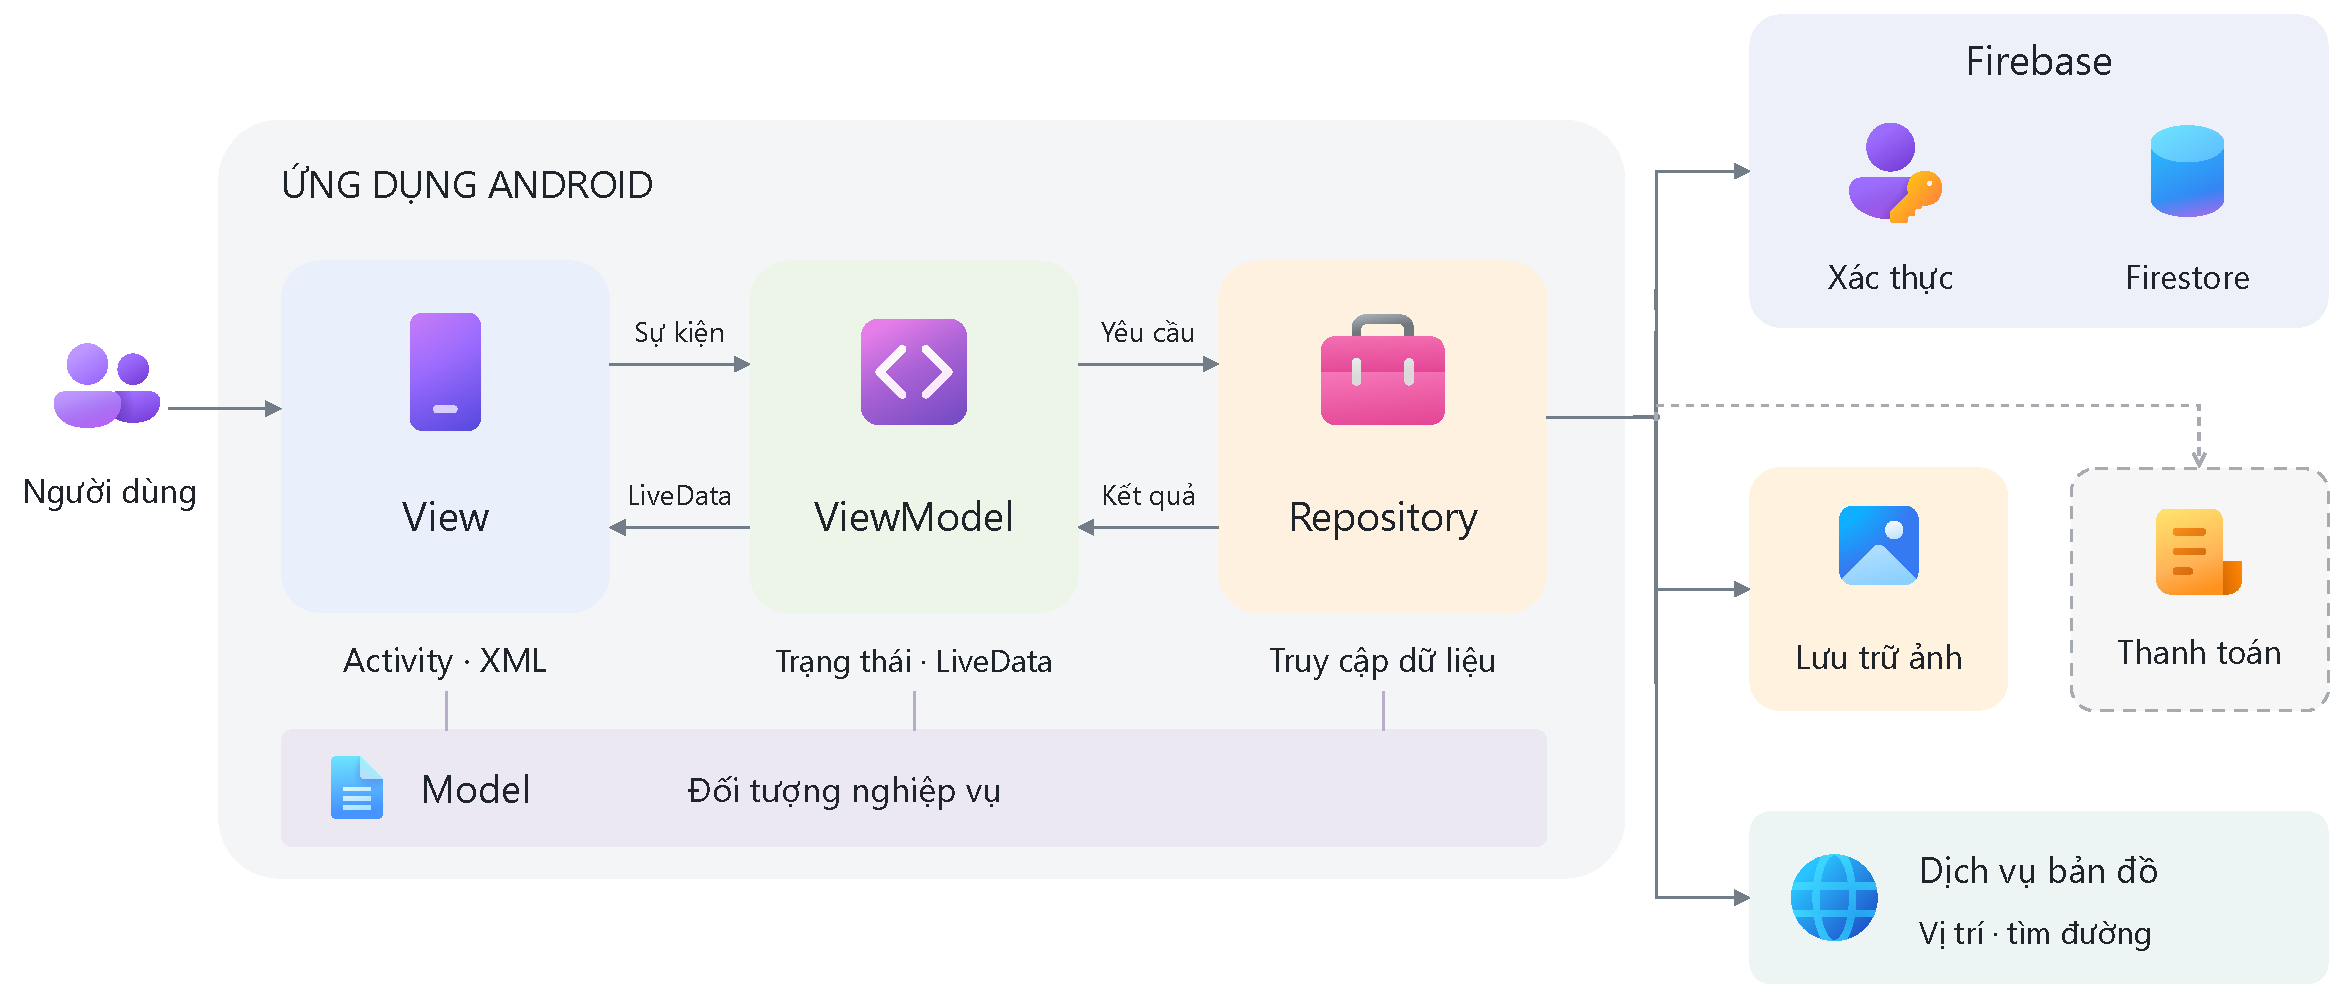
\includegraphics[width=\textwidth]{chapter5/application-architecture.pdf}
\caption{Kiến trúc tổng quan của ứng dụng BroomSharing}\label{fig:mvvm}
\end{figure}

Mũi tên từ View đến ViewModel biểu diễn lời gọi phương thức xử lý tương tác; chiều ngược lại biểu diễn dữ liệu trạng thái để View quan sát. ViewModel giao tiếp với Repository, không cần phụ thuộc vào API Firestore. Model được các thành phần sử dụng để biểu diễn dữ liệu nghiệp vụ. Nhánh thanh toán dùng nét đứt để thể hiện phần tích hợp dự kiến, chưa xác định nhà cung cấp.

\subsection{Cấu trúc thư mục đề xuất}
\begin{table}[H]\centering\small
\caption{Tổ chức gói mã nguồn Java + XML theo trách nhiệm}\label{tab:packages}
\begin{tabularx}{\textwidth}{@{}p{4.9cm}X@{}}\toprule
\textbf{Nhóm thư mục}&\textbf{Nhiệm vụ}\cr\midrule
\texttt{ui/} & Activity, Fragment, Adapter, ViewHolder và thành phần điều hướng.\\
\texttt{viewmodel/} & Ví dụ \texttt{SpaceViewModel}, \texttt{BookingViewModel}; cung cấp LiveData hoặc trạng thái tương ứng.\\
\texttt{repository/} & Ví dụ \texttt{SpaceRepository}, \texttt{BookingRepository}; đọc/ghi dữ liệu qua Firebase SDK.\\
\texttt{model/} & Các POJO \texttt{User}, \texttt{Space}, \texttt{Booking}, \texttt{Review} nếu cần.\\
\texttt{res/layout/} & XML cho Activity, Fragment, item danh sách và hộp thoại.\\
\texttt{res/drawable/}, \texttt{res/values/} & Ảnh, icon, màu, chuỗi và theme của ứng dụng.\\\bottomrule
\end{tabularx}\end{table}

\subsection{Kết nối với Firebase}
Ứng dụng Android cần được liên kết với dự án Firebase, cấu hình thư viện theo hướng dẫn chính thức và kiểm tra quyền đọc/ghi. Repository là nơi phù hợp để gọi \texttt{FirebaseFirestore} qua phương thức \texttt{getInstance()}, thực hiện truy vấn và ánh xạ tài liệu sang đối tượng Java. Hoạt động bất đồng bộ phải trả kết quả bằng callback/LiveData hoặc cơ chế tương đương; không thực hiện chờ mạng trên luồng giao diện \parencite{firebase_android,firebase_firestore}.

Đối với ảnh không gian, nên phân biệt tệp ảnh với bản ghi dữ liệu: tệp được quản lý bởi dịch vụ lưu trữ phù hợp; URL hoặc đường dẫn được tham chiếu trong \texttt{spaces}. Nếu phiên bản đồ án chỉ dùng ảnh tĩnh trong \texttt{drawable}, báo cáo phải mô tả đúng lựa chọn đó thay vì khẳng định có tải ảnh lên Storage.

\subsection{Minh họa luồng nghiệp vụ ``xem danh sách không gian''}
\begin{enumerate}[leftmargin=*]
\item Activity/Fragment tạo hoặc lấy ViewModel gắn với vòng đời giao diện.
\item View đăng ký quan sát danh sách không gian qua LiveData.
\item ViewModel gọi phương thức lấy danh sách ở SpaceRepository.
\item Repository truy vấn Firestore, ánh xạ document thành các đối tượng Space.
\item Khi có dữ liệu hoặc lỗi, ViewModel cập nhật trạng thái; View hiển thị thông tin qua RecyclerView hoặc trạng thái rỗng/lỗi tương ứng.
\end{enumerate}
Luồng này là \textbf{phương án tổ chức mã nguồn kiến trúc}; chưa phải bằng chứng rằng toàn bộ Activity hiện tại đã được refactor theo MVVM.

\subsection{Tích hợp bản đồ và ảnh trong kiến trúc}
Phần bản đồ và quản lý ảnh được bố trí như các dịch vụ tích hợp, không thay đổi nguyên tắc phân lớp chính của MVVM. Tab \textbf{Map} sử dụng \texttt{MapView} của MapLibre trong XML và Activity/Fragment Java để hiển thị bản đồ. Repository truy xuất danh sách không gian có tọa độ từ Firestore; lớp giao diện nhận dữ liệu đã được ViewModel cung cấp và đặt marker. Khi chọn tìm đường, thành phần tích hợp openrouteservice nhận điểm đi/đến, đọc GeoJSON và chuyển hình học tuyến để hiển thị trên MapLibre. MapTiler cung cấp style/tile và có thể hỗ trợ chuyển đổi địa chỉ thành tọa độ \parencite{maplibre_android,maptiler_geocoding,ors_directions}.

Ảnh không gian được chọn ở giao diện, tải lên Cloudinary theo cấu hình cho phép; sau khi thành công, ứng dụng cập nhật URL vào tài liệu \texttt{spaces} trên Firestore. Chỉ nên đưa vào báo cáo cuối kỳ các bước đã có mã nguồn và kết quả chạy. Việc gọi API mạng phải bất đồng bộ; không lưu khóa bí mật dịch vụ ở dạng hard-code trong ứng dụng \parencite{cloudinary_android}.

\begin{table}[H]\centering\small
\caption{Vai trò các công nghệ và luồng phụ trợ trong kiến trúc}\label{tab:services}
\begin{tabularx}{\textwidth}{@{}p{4.0cm}X@{}}\toprule
\textbf{Thành phần}&\textbf{Trách nhiệm trong thiết kế}\\\midrule
MapLibre Native & Thành phần Android View để hiển thị bản đồ, marker và đường đi.\\
MapTiler & Cung cấp dữ liệu bản đồ và geocoding theo API key.\\
openrouteservice & Trả dữ liệu tuyến đường giữa các tọa độ, ví dụ GeoJSON.\\
Android Location & Lấy tọa độ của thiết bị khi đã có quyền phù hợp.\\
Cloudinary & Upload và lưu trữ tệp ảnh, trả URL để ghi vào Firestore.\\
Cloud Firestore & Lưu các bản ghi nghiệp vụ, thuộc tính tọa độ và URL ảnh.\\\bottomrule
\end{tabularx}\end{table}

\subsection{Các màn hình và mức độ hoàn thiện}
Màn hình khám phá, chi tiết, bản đồ, đặt chỗ, đăng không gian, lịch sử booking, tin nhắn, hồ sơ và quản trị đã được thảo luận ở giai đoạn thiết kế UI. Để ghi nhận là \textit{đã xây dựng}, từng màn hình cần có tệp layout/Activity thật, ảnh chụp và một mục kiểm thử. Giai đoạn thiết kế có thể chấp nhận việc một số màn hình chỉ có bố cục XML hoặc dữ liệu mẫu; giai đoạn báo cáo thực thi phải mô tả khác biệt này rõ ràng.

\chapstart
\section{QUY TRÌNH THỰC THI VÀ KIỂM THỬ}
\subsection{Quy trình đăng ký và đăng nhập}
Người dùng nhập thông tin cơ bản, hệ thống kiểm tra dữ liệu hợp lệ và xác lập phiên đăng nhập. Sau khi đăng nhập, giao diện có thể điều chỉnh theo quyền User hoặc Owner. Nếu tích hợp Firebase Authentication, danh tính đăng nhập cần liên hệ nhất quán với document hồ sơ trong \texttt{users}; tài khoản không được coi là hợp lệ chỉ dựa vào dữ liệu do client tự khai báo \parencite{firebase_security}.

\subsection{Quy trình tìm kiếm và đặt thuê không gian}
\begin{enumerate}[leftmargin=*]
\item \textbf{Khám phá:} người dùng mở danh sách, tra cứu từ khóa hoặc lọc địa điểm, giá, kỳ thuê.
\item \textbf{Đối chiếu:} xem mô tả, ảnh, giá và điều kiện sử dụng của không gian được chọn.
\item \textbf{Chọn thời gian:} nhập ngày bắt đầu/kết thúc theo quy ước đặt phòng hoặc kỳ thuê.
\item \textbf{Kiểm tra:} đánh giá tính hợp lệ, điều kiện sẵn có và giá dự kiến.
\item \textbf{Gửi yêu cầu:} tạo document booking với trạng thái ban đầu phù hợp.
\item \textbf{Theo dõi:} hiển thị trạng thái cập nhật trong lịch sử đặt chỗ.
\end{enumerate}

\subsection{Quy trình đăng và quản lý không gian}
Chủ không gian tạo bản ghi mới bằng cách nhập tên, địa chỉ, ảnh, tiện ích, thời gian sẵn có và giá theo đơn vị quy định. Trước khi công bố, thông tin bắt buộc cần hợp lệ. Khi nhận booking, chủ không gian xem chi tiết yêu cầu, cập nhật trạng thái theo quyền được phép và theo dõi các mốc thời gian đã được xác nhận. Nếu áp dụng duyệt tin bởi Admin, trạng thái ``chờ duyệt'' sẽ được xét riêng thay vì công bố trực tiếp.

\subsection{Quy trình xác nhận và QR check-in}
Sau khi booking được chấp thuận, hệ thống có thể cung cấp một mã tham chiếu hoặc mã QR cho bước nhận không gian. Phương án QR cần gắn với booking cụ thể, có hạn sử dụng và chỉ chấp nhận xác nhận một lần theo đúng chính sách. Chức năng này được giữ ở mức \textbf{định hướng nghiệp vụ}, do chưa có căn cứ về việc quét, sinh mã và xác nhận tại thiết bị đã được cài đặt đầy đủ.

\subsection{Thiết kế các ca kiểm thử}
Các bảng dưới đây là bộ ca kiểm thử cần thực hiện trên emulator/thiết bị và tài khoản thử nghiệm. Cột kết quả được để trống có chủ ý: chỉ ghi nhận sau khi thu thập ảnh hoặc log thực thi.
\begin{longtable}{@{}p{1.5cm}p{5.0cm}p{5.5cm}p{2.5cm}@{}}
\caption{Ma trận kiểm thử chức năng}\label{tab:tests}\\\toprule
\textbf{Mã}&\textbf{Tình huống}&\textbf{Kết quả mong đợi}&\textbf{Kết quả thực tế}\cr\midrule\endfirsthead
\toprule\textbf{Mã}&\textbf{Tình huống}&\textbf{Kết quả mong đợi}&\textbf{Kết quả thực tế}\cr\midrule\endhead
TC-01& Vào màn hình khám phá khi có dữ liệu.& Danh sách hiển thị đầy đủ thông tin chính.&Chưa kiểm thử\\
TC-02& Bộ lọc không khớp tin nào.& Hiện thông báo rỗng, không crash.&Chưa kiểm thử\\
TC-03& Mở màn hình chi tiết từ một item.& Hiển thị đúng mã không gian được chọn.&Chưa kiểm thử\\
TC-04& Chọn ngày kết thúc trước ngày bắt đầu.& Chặn yêu cầu, giải thích lỗi.&Chưa kiểm thử\\
TC-05& Đặt trùng khung thời gian đã xác nhận.& Không phát sinh booking xác nhận trùng.&Chưa kiểm thử\\
TC-06& Owner sửa tin của người khác.& Hệ thống từ chối ghi dữ liệu.&Chưa kiểm thử\\
TC-07& Mất kết nối khi gửi yêu cầu.& Hiển thị trạng thái lỗi/thử lại phù hợp.&Chưa kiểm thử\\
TC-08& Đăng tin thiếu tên hoặc giá.& Báo trường bắt buộc, không ghi sai dữ liệu.&Chưa kiểm thử\\
TC-09& Xoay màn hình khi đang xem danh sách.& Trạng thái UI không sai lệch nghiêm trọng.&Chưa kiểm thử\\
TC-10& QR đã dùng hoặc hết hạn (nếu tích hợp).& Không chấp nhận tái sử dụng.&Chưa kiểm thử\\
TC-11& Bật bản đồ và cho phép truy cập vị trí.& Đọc tọa độ hợp lệ, hiển thị marker không gian.&Chưa kiểm thử\\
TC-12& Yêu cầu chỉ đường đến không gian.& Dữ liệu tuyến trả về được xử lý hoặc hiển thị lỗi mạng phù hợp.&Chưa kiểm thử\\
TC-13& Thêm ảnh từ thiết bị lên Cloudinary.& Chỉ ghi URL vào Firestore sau khi upload thành công.&Chưa kiểm thử\\\bottomrule
\end{longtable}

\subsection{Đánh giá giới hạn và chứng cứ thực thi}
Một báo cáo hoàn chỉnh cần có hình chụp giao diện từ thiết bị/emulator, một ví dụ document Firestore đã lưu và minh chứng kiểm tra ít nhất một quy trình đầu-cuối. Ở bản dựng này, thông tin đó chưa có trong tài liệu đầu vào, vì vậy chưa thể kết luận về tỷ lệ kiểm thử đạt, độ ổn định hay thời gian đáp ứng của hệ thống. Không gán các chỉ số giả định để thay thế cho kết quả đo thật.

\chapstart
\section{KẾT LUẬN VÀ HƯỚNG MỞ RỘNG}
\subsection{Kết luận của giai đoạn thiết kế}
BroomSharing đề xuất một mô hình ứng dụng Android để khai thác và chia sẻ không gian còn trống theo ngày hoặc tháng. Báo cáo xác định được nhóm tác nhân User, Owner và Admin (mở rộng), các thao tác chính gồm tìm kiếm, đọc chi tiết, đăng không gian, gửi yêu cầu thuê và quản lý booking. Lược đồ dữ liệu dự kiến tập trung vào các collection \texttt{users}, \texttt{spaces} và \texttt{bookings}, cho phép mô tả rõ các liên kết logic cốt lõi.

Về kiến trúc, cách tổ chức Java + XML theo MVVM + Repository + Model giúp tách công việc hiển thị giao diện khỏi việc truy cập Firebase \parencite{android_arch,android_data}. Tuy nhiên, đây là kết quả phân tích và thiết kế, không thay cho việc kiểm tra implementation, kiểm thử và khả năng hoạt động thực tế của ứng dụng ở thời điểm nộp bài.

\subsection{Những hạn chế hiện tại}
Bản báo cáo được biên soạn từ tài liệu mẫu môn học và thông tin nghiệp vụ đã trao đổi, không được cung cấp trực tiếp mã nguồn BroomSharing hoặc bản xuất Firestore để đối chiếu. Vì vậy tên lớp, bộ sưu tập dữ liệu, trạng thái booking và sự hiện diện của các màn hình là phương án đề xuất. Không có căn cứ xác nhận thanh toán trong ứng dụng, đồng bộ lịch theo thời gian thực, chat hoàn chỉnh, QR check-in, quy trình duyệt tin hoặc kiểm thử thiết bị đã hoàn thành.

\subsection{Hướng phát triển}
\begin{itemize}
\item Hoàn thiện luồng bản đồ MapLibre, marker từ Firestore, MapTiler geocoding và openrouteservice directions; kiểm chứng giới hạn API key và quota trên môi trường thử nghiệm.
\item Hoàn thiện upload ảnh Cloudinary có kiểm soát, thử nghiệm các tình huống lỗi mạng và giới hạn dung lượng.
\item Hoàn thiện bộ lọc theo vị trí, giá, kỳ thuê và tiện ích, đồng thời tối ưu dữ liệu tìm kiếm.
\item Xây dựng cơ chế kiểm tra chồng lấn booking đáng tin cậy tại tầng dữ liệu hoặc backend.
\item Cải thiện chất lượng tin đăng bằng quy trình duyệt nội dung và báo cáo thông tin không chính xác.
\item Bổ sung thông báo trạng thái booking, đánh giá sau sử dụng và lịch sử giao dịch.
\item Nghiên cứu QR check-in/check-out có điều kiện và cơ chế ngăn sử dụng lại mã.
\item Thực hiện kiểm thử chức năng, bảo mật và hiệu năng trước khi phát hành thử nghiệm.
\end{itemize}

\clearpage
\phantomsection
\printbibliography[heading=bibintoc,title={TÀI LIỆU THAM KHẢO}]
% PHU LUC - bo cuc va thong tin theo AI_PROJECT, co bo sung noi dung mau cua thay.
\clearpage
\pagestyle{plain}
\setcounter{table}{0}\renewcommand{\thetable}{PL.\arabic{table}}
\section*{PHỤ LỤC A. HÌNH ẢNH}
\phantomsection\addcontentsline{toc}{section}{PHỤ LỤC A. HÌNH ẢNH}
\setcounter{figure}{0}\renewcommand{\thefigure}{A.\arabic{figure}}
\printappendixfigures
\clearpage
\subsection*{A.1. Thiết kế giao diện Admin}
Hình~\ref{fig:app-admin-design} minh họa hai nhóm nội dung kiểm duyệt phòng và quản lý tài khoản. Thẻ thông tin đặt thao tác chấp thuận, từ chối hoặc quản lý trạng thái cạnh đối tượng cần xử lý. Phần tổng quan và bộ lọc hỗ trợ xác định nhóm hồ sơ trước khi mở chi tiết; số liệu trong hình là dữ liệu minh họa thiết kế.
\begin{figure}[H]\centering
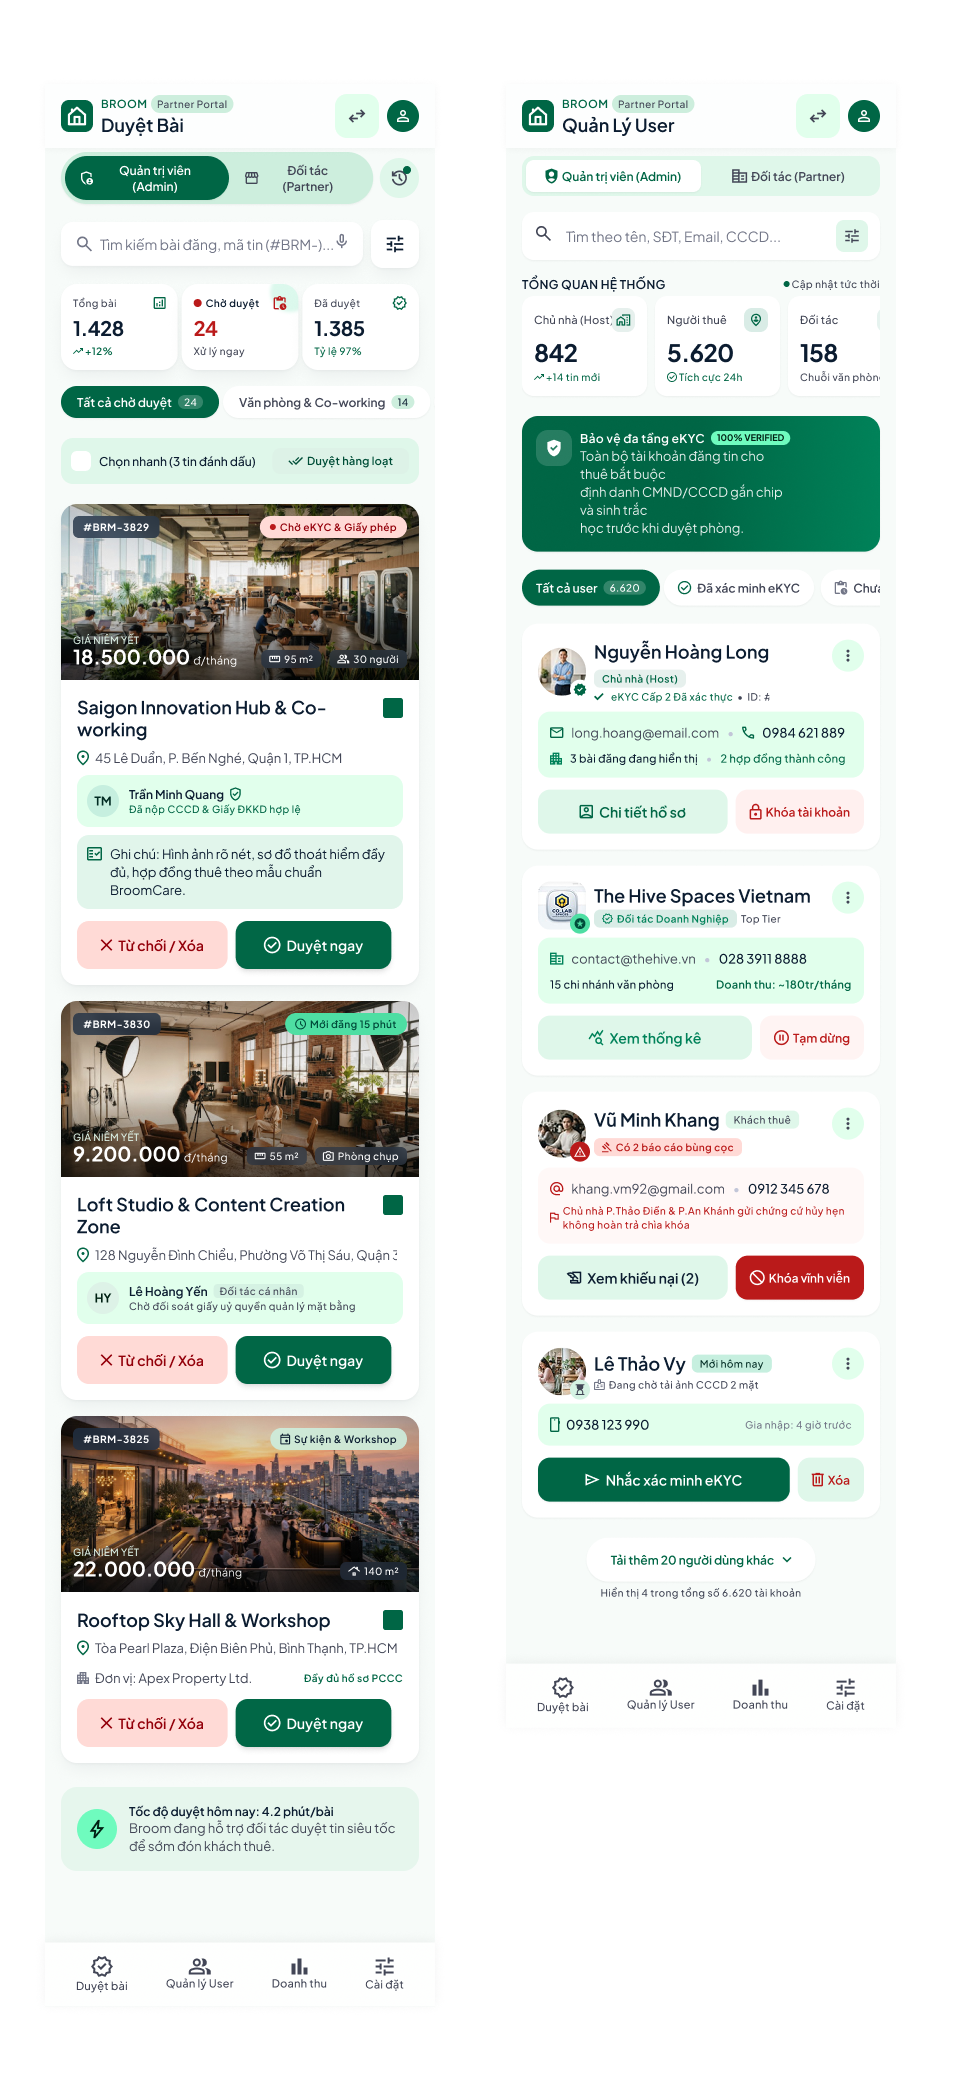
\includegraphics[width=\textwidth,height=0.76\textheight,keepaspectratio]{chapter3/admin-design.png}
\caption{Phương án thiết kế kiểm duyệt và quản lý trong phân hệ Admin.}\label{fig:app-admin-design}
\end{figure}

\clearpage


\clearpage
\section*{PHỤ LỤC B. TRUY VẤN SQL VÀ TRUY VẤN FIRESTORE}
\phantomsection\addcontentsline{toc}{section}{PHỤ LỤC B. TRUY VẤN SQL VÀ FIRESTORE}
\appendixnote{Phụ lục minh họa các thao tác truy vấn dữ liệu trong BroomSharing. Vì kiến trúc sử dụng Cloud Firestore (NoSQL), các câu SQL chỉ biểu diễn logic tương đương, không phải mã có thể thực thi trực tiếp trên Firestore.}
\subsection*{B.1. Liệt kê không gian đang được công bố}
\begin{minted}{sql}
-- Pseudo-SQL: minh hoa truy van tuong duong
SELECT space_id, title, address, price, status
FROM spaces
WHERE status = 'available'
ORDER BY created_at DESC;
\end{minted}
\noindent\textbf{Lệnh Java/Firestore tương ứng (minh họa):}
\begin{minted}{java}
FirebaseFirestore db = FirebaseFirestore.getInstance();
db.collection("spaces")
  .whereEqualTo("status", "available")
  .orderBy("createdAt", Query.Direction.DESCENDING)
  .get()
  .addOnSuccessListener(result -> {
      // Anh xa document sang Model Space
  });
\end{minted}
\noindent\textit{Lưu ý:} tổ hợp lọc và sắp xếp có thể đòi hỏi tạo composite index trên Firestore theo hướng dẫn của Firebase.

\subsection*{B.2. Tìm kiếm không gian theo mức giá}
\begin{minted}{sql}
-- Pseudo-SQL: minh hoa logic loc theo muc gia
SELECT space_id, title, price
FROM spaces
WHERE status = 'available'
  AND price BETWEEN :min_price AND :max_price
ORDER BY price ASC;
\end{minted}
\noindent\textbf{Hướng truy vấn Firestore:} dùng \texttt{whereGreaterThanOrEqualTo}, \texttt{whereLessThanOrEqualTo} và \texttt{orderBy} trên trường giá. Trước khi triển khai phải thống nhất đơn vị tiền tệ và kỳ thuê để dữ liệu có thể so sánh được.

\Needspace{9\baselineskip}
\subsection*{B.3. Danh sách booking của một người dùng}
\begin{minted}{sql}
-- Pseudo-SQL: minh hoa logic truy van
SELECT booking_id, space_id, start_time, end_time, status
FROM bookings
WHERE renter_id = :current_user_id
ORDER BY created_at DESC;
\end{minted}
\noindent\textbf{Hướng truy vấn Firestore:} lọc theo \texttt{renterId} của người dùng hiện tại, sau đó sắp xếp theo \texttt{createdAt}; quy tắc Security Rules phải kiểm tra quyền đọc của tài khoản. Thao tác đặt trùng thời gian cần được xử lý nhất quán và không chỉ dựa vào kiểm tra ở giao diện \parencite{firebase_security,firebase_transaction}.

\subsection*{B.4. Liệt kê không gian do một chủ sở hữu quản lý}
\begin{minted}{sql}
-- Pseudo-SQL: danh sach tin dang cua Owner
SELECT space_id, title, price, status, created_at
FROM spaces
WHERE owner_id = :current_owner_id
ORDER BY created_at DESC;
\end{minted}
\noindent\textbf{Hướng truy vấn Firestore:} sử dụng điều kiện lọc \texttt{ownerId} theo định danh đăng nhập và sắp xếp \texttt{createdAt}. Quyền sửa tin cần được kiểm tra bằng Security Rules thay vì chỉ kiểm soát nút trên giao diện \parencite{firebase_security}.

\subsection*{B.5. Cập nhật trạng thái yêu cầu đặt thuê}
\begin{minted}{sql}
-- Pseudo-SQL: Owner xu ly yeu cau booking
UPDATE bookings
SET status = 'approved', updated_at = :now
WHERE booking_id = :booking_id
  AND status = 'pending'
  AND owner_id = :current_owner_id;
\end{minted}
\noindent\textbf{Hướng xử lý Firestore:} trước khi chuyển trạng thái, xác nhận quyền của chủ không gian và trạng thái hiện tại; nếu có dữ liệu phụ thuộc hoặc điều kiện cạnh tranh, xét cơ chế transaction và kiểm tra tính nhất quán \parencite{firebase_transaction,firebase_security}. Câu truy vấn trên chỉ dùng để giải thích điều kiện nghiệp vụ.

\clearpage
\section*{PHỤ LỤC C. DANH MỤC BẢNG, BIỂU}
\phantomsection\addcontentsline{toc}{section}{PHỤ LỤC C. DANH MỤC BẢNG, BIỂU}
\appendixnote{Danh mục bảng biểu trong phần thân báo cáo được sinh tự động; số trang và số thứ tự sẽ cập nhật theo kết quả biên dịch cuối cùng.}
\printappendixtables

\clearpage
\section*{PHỤ LỤC D. ĐƯỜNG DẪN TÀI NGUYÊN ĐỒ ÁN}
\phantomsection\addcontentsline{toc}{section}{PHỤ LỤC D. ĐƯỜNG DẪN TÀI NGUYÊN ĐỒ ÁN}
\appendixnote{Các tài nguyên trực tuyến hỗ trợ theo dõi tiến độ, đối chiếu mã nguồn và kiểm tra minh chứng thực hiện của nhóm.}

\subsection*{Bảng phân công nhiệm vụ}
Bảng phân công được nhóm lưu trực tuyến để giảng viên theo dõi nhiệm vụ, tiến độ và kết quả của từng thành viên.
\begin{center}
{\Large\bfseries
\ifdefempty{\BroomSheetURL}{\faFileExcel\ XEM BẢNG PHÂN CÔNG CÔNG VIỆC}{\href{\BroomSheetURL}{\faFileExcel\ XEM BẢNG PHÂN CÔNG CÔNG VIỆC}}
}
\end{center}

\subsection*{Link đồ án -- GitHub}
Mã nguồn BroomSharing được quản lý bằng GitHub nhằm phục vụ việc xem xét các thành phần dự án và lịch sử phát triển.
\begin{center}
{\Large\bfseries
\ifdefempty{\BroomGitHubURL}{\faGithub\ XEM SOURCE CODE BROOMSHARING}{\href{\BroomGitHubURL}{\faGithub\ XEM SOURCE CODE BROOMSHARING}}
}
\end{center}

\subsection*{Đường dẫn học phần}
Các tài liệu và yêu cầu được giảng viên công bố là cơ sở để đối chiếu cấu trúc và tiêu chí đánh giá đồ án.
\begin{center}
{\large\bfseries
\ifdefempty{\BroomCourseURL}{\faGraduationCap\ XEM THÔNG TIN HỌC PHẦN}{\href{\BroomCourseURL}{\faGraduationCap\ XEM THÔNG TIN HỌC PHẦN}}
}
\end{center}

\subsection*{GitHub Projects và thư mục minh chứng}
Bảng công việc và tập ảnh ghi nhận tiến độ được quản lý độc lập với báo cáo để thuận tiện cập nhật.
\begin{center}
{\large\bfseries
\ifdefempty{\BroomProjectsURL}{\faTasks\ XEM NHẬT KÝ PHÂN CÔNG}{\href{\BroomProjectsURL}{\faTasks\ XEM NHẬT KÝ PHÂN CÔNG}}
}\par\smallskip
{\large\bfseries
\ifdefempty{\BroomImagesURL}{\faImages\ XEM THƯ MỤC ẢNH MINH CHỨNG}{\href{\BroomImagesURL}{\faImages\ XEM THƯ MỤC ẢNH MINH CHỨNG}}
}
\end{center}


\clearpage
\section*{PHỤ LỤC E. BẢNG PHÂN CÔNG VÀ MINH CHỨNG NHÓM}
\phantomsection\addcontentsline{toc}{section}{PHỤ LỤC E. BẢNG PHÂN CÔNG VÀ MINH CHỨNG NHÓM}
\appendixnote{Bảng phân công nêu trách nhiệm và sản phẩm bàn giao của từng thành viên; minh chứng cần đối chiếu được với GitHub Projects, Google Sheets hoặc lịch sử commit.}
\begin{longtable}{@{}>{\raggedright\arraybackslash}p{4.2cm}p{6.7cm}p{3.2cm}@{}}\caption{Bảng nhiệm vụ nhóm cần xác nhận}\label{tab:append_assign}\\\toprule
\textbf{Thành viên}&\textbf{Nhiệm vụ riêng}&\textbf{Commit / Issues / Sheet}\\\midrule\endfirsthead
\toprule\textbf{Thành viên}&\textbf{Nhiệm vụ riêng}&\textbf{Commit / Issues / Sheet}\\\midrule\endhead
Lữ Võ Hoàng Phúc& Bổ sung phần việc thực tế theo log triển khai BroomSharing.& Chưa cung cấp\\
Lâm Hoàng& Ghi đúng hạng mục đã nhận và kết quả bàn giao.& Chưa cung cấp\\
Từ Trương Thanh Trúc& Ghi đúng hạng mục đã nhận và kết quả bàn giao.& Chưa cung cấp\\
\bottomrule\end{longtable}
\noindent\textbf{Minh chứng nên kèm:} ảnh phân công GitHub Projects hoặc Google Sheets; ảnh lịch sử commit thể hiện tên người thực hiện, thời gian và tệp thay đổi; liên kết commit tương ứng. Không suy đoán kết quả của từng thành viên khi chưa có dữ liệu.

\clearpage
\section*{PHỤ LỤC F. TƯ LIỆU VÀ KIỂM TRA BỔ SUNG}
\phantomsection\addcontentsline{toc}{section}{PHỤ LỤC F. TƯ LIỆU VÀ KIỂM TRA BỔ SUNG}
\appendixnote{Các tài liệu vượt khỏi dung lượng báo cáo chính hoặc minh chứng phát sinh trong quá trình triển khai được đặt tại đây để không làm gián đoạn dòng trình bày của bảy chương.}
\begin{enumerate}[leftmargin=*]
\item Nhật ký thử nghiệm trên emulator và thiết bị thực: phiên bản Android, loại thiết bị, thao tác thực hiện, kết quả, ảnh/log.
\item Trích xuất cấu trúc collection/document Firestore và Security Rules đã kiểm tra; không công khai khóa bí mật.
\item Ảnh chụp bổ sung về màn hình tìm kiếm, hồ sơ, chủ không gian, xử lý booking, bản đồ hoặc QR (chỉ khi đã thực hiện).
\item Các đoạn truy vấn hoặc mã Java/Repository quá dài: chuyển sang mã nguồn GitHub và liên kết đến dòng code tương ứng.
\item Kịch bản kiểm thử bổ sung, lỗi đã phát hiện và cách khắc phục; ghi tách biệt với chức năng chỉ mới được đề xuất.
\end{enumerate}

\clearpage
\section*{PHỤ LỤC G. PHÂN RÃ CHỨC NĂNG CHI TIẾT}
\phantomsection\addcontentsline{toc}{section}{PHỤ LỤC G. PHÂN RÃ CHỨC NĂNG CHI TIẾT}
\label{app:chapter2-details}
\setcounter{figure}{0}\renewcommand{\thefigure}{G.\arabic{figure}}
Các nhóm chức năng dưới đây triển khai chi tiết từ sơ đồ tổng quát ở Chương 2. Mỗi nhóm gắn với một phạm vi nghiệp vụ; các bước dùng chung được giữ trong cùng nhóm để thể hiện trách nhiệm xử lý.

\clearpage
Nhóm tài khoản quản lý đăng nhập, đăng ký, khôi phục mật khẩu và phiên truy cập theo vai trò.
\begin{figure}[H]\centering
\includegraphics[page=2,width=\textwidth,height=0.78\textheight,keepaspectratio]{chapter2/usecase_decomposition_v2.pdf}
\caption{Phân rã chức năng: tài khoản và phiên.}\label{fig:app-functions-2}
\end{figure}

\clearpage
Khám phá không gian kết hợp tìm kiếm, bộ lọc, bản đồ và thông tin phòng trước khi đặt.
\begin{figure}[H]\centering
\includegraphics[page=3,width=\textwidth,height=0.78\textheight,keepaspectratio]{chapter2/usecase_decomposition_v2.pdf}
\caption{Phân rã chức năng: khám phá không gian.}\label{fig:app-functions-3}
\end{figure}

\clearpage
Yêu cầu đặt chỗ bao gồm chọn kỳ thuê, kiểm tra khả dụng, chốt giá và mở QR với thời hạn giữ lịch tạm.
\begin{figure}[H]\centering
\includegraphics[page=4,width=\textwidth,height=0.78\textheight,keepaspectratio]{chapter2/usecase_decomposition_v2.pdf}
\caption{Phân rã chức năng: tạo yêu cầu đặt chỗ.}\label{fig:app-functions-4}
\end{figure}

\clearpage
Theo dõi lượt thuê phân biệt lịch sử, thời hạn thanh toán và điều kiện hủy; nhả lịch đi cùng cập nhật trạng thái.
\begin{figure}[H]\centering
\includegraphics[page=5,width=\textwidth,height=0.78\textheight,keepaspectratio]{chapter2/usecase_decomposition_v2.pdf}
\caption{Phân rã chức năng: lịch đặt và hủy.}\label{fig:app-functions-5}
\end{figure}

\clearpage
Hồ sơ Host được xét duyệt riêng với minh chứng vị trí hoặc hình ảnh của tài sản.
\begin{figure}[H]\centering
\includegraphics[page=6,width=\textwidth,height=0.78\textheight,keepaspectratio]{chapter2/usecase_decomposition_v2.pdf}
\caption{Phân rã chức năng: hồ sơ host và xác minh.}\label{fig:app-functions-6}
\end{figure}

\clearpage
Quản lý tài sản tách tòa nhà, phòng, cấu hình giá và lịch; công bố phòng phụ thuộc trạng thái xét duyệt và hoạt động.
\begin{figure}[H]\centering
\includegraphics[page=7,width=\textwidth,height=0.78\textheight,keepaspectratio]{chapter2/usecase_decomposition_v2.pdf}
\caption{Phân rã chức năng: quản lý không gian.}\label{fig:app-functions-7}
\end{figure}

\clearpage
Vận hành lượt thuê phân biệt nhận phòng, hoàn tất và không đến, không suy ra đã sử dụng chỉ từ thời gian.
\begin{figure}[H]\centering
\includegraphics[page=8,width=\textwidth,height=0.78\textheight,keepaspectratio]{chapter2/usecase_decomposition_v2.pdf}
\caption{Phân rã chức năng: theo dõi và sử dụng.}\label{fig:app-functions-8}
\end{figure}

\clearpage
Chat gắn với cặp thành viên, cập nhật tin cuối và mốc đọc; liên hệ không cấp quyền đọc hội thoại cho bên ngoài.
\begin{figure}[H]\centering
\includegraphics[page=9,width=\textwidth,height=0.78\textheight,keepaspectratio]{chapter2/usecase_decomposition_v2.pdf}
\caption{Phân rã chức năng: chat và liên hệ.}\label{fig:app-functions-9}
\end{figure}

\clearpage
Đánh giá chỉ gắn với lượt đã khép và có xác nhận sử dụng, nhằm tách trải nghiệm thật khỏi lượt không đến.
\begin{figure}[H]\centering
\includegraphics[page=10,width=\textwidth,height=0.78\textheight,keepaspectratio]{chapter2/usecase_decomposition_v2.pdf}
\caption{Phân rã chức năng: đánh giá sau sử dụng.}\label{fig:app-functions-10}
\end{figure}

\clearpage
Báo cáo là hồ sơ xử lý vi phạm có phản hồi của Host và kết luận của Admin, tách với nội dung đánh giá.
\begin{figure}[H]\centering
\includegraphics[page=11,width=\textwidth,height=0.78\textheight,keepaspectratio]{chapter2/usecase_decomposition_v2.pdf}
\caption{Phân rã chức năng: báo cáo và phản hồi.}\label{fig:app-functions-11}
\end{figure}

\clearpage
Quản trị bao gồm kiểm duyệt, hạn chế hoạt động và xử lý từng ngoại lệ của booking, có lưu lý do.
\begin{figure}[H]\centering
\includegraphics[page=12,width=\textwidth,height=0.78\textheight,keepaspectratio]{chapter2/usecase_decomposition_v2.pdf}
\caption{Phân rã chức năng: quản trị và sự cố.}\label{fig:app-functions-12}
\end{figure}

\clearpage
Theo dõi và nhật ký phục vụ đối chiếu thay đổi; bộ đếm và lịch giữ chỗ phải khớp với các booking đang hiệu lực.
\begin{figure}[H]\centering
\includegraphics[page=13,width=\textwidth,height=0.78\textheight,keepaspectratio]{chapter2/usecase_decomposition_v2.pdf}
\caption{Phân rã chức năng: theo dõi và nhật ký.}\label{fig:app-functions-13}
\end{figure}

\clearpage
Hồ sơ và thông báo tổng hợp thông tin cá nhân, ảnh đại diện và các cập nhật liên quan đến tài khoản.
\begin{figure}[H]\centering
\includegraphics[page=14,width=\textwidth,height=0.78\textheight,keepaspectratio]{chapter2/usecase_decomposition_v2.pdf}
\caption{Phân rã chức năng: hồ sơ và thông báo.}\label{fig:app-functions-14}
\end{figure}

\clearpage
Thanh toán demo dùng một kênh payOS: tạo QR, đối soát nhận tiền và cập nhật kết quả; không tự hoàn tiền.
\begin{figure}[H]\centering
\includegraphics[page=15,width=\textwidth,height=0.78\textheight,keepaspectratio]{chapter2/usecase_decomposition_v2.pdf}
\caption{Phân rã chức năng: thanh toán demo.}\label{fig:app-functions-15}
\end{figure}


\end{document}
